\documentclass[11pt,a4paper,oneside]{ltjsarticle}
\usepackage{graphicx}
\usepackage{amsmath, amssymb}
\usepackage{geometry}
\usepackage{setspace} % 行間調整
\usepackage{luatexja-preset} % 日本語設定
\usepackage{here}    % 図の配置 [H]
\usepackage{tocloft} % 目次のカスタマイズ   
\usepackage{comment} % comment 環境を使用するために追加
\usepackage[compatibility=false]{caption}
\usepackage{subcaption} 
\usepackage{enumerate}
\usepackage{enumitem}
\usepackage{float}
\DeclareMathOperator*{\argmin}{argmin} % argmin コマンドを定義


% 図番号を章ごとにリセット
\renewcommand{\thefigure}{\thesection.\arabic{figure}}
\counterwithin{figure}{section}

\setlength{\textwidth}{150mm}
\setlength{\textheight}{240mm}
\setlength{\oddsidemargin}{5mm}
\setlength{\evensidemargin}{5mm}
\setlength{\topmargin}{3mm}

%上5行でテキストの配置位置の設定をしています。図の体裁などがどうしても合わないときはちょっといじってみるといいでしょう。

%jbookでは 「参考文献」ではなく「関連図書」と表示されてしまうのでこれが必要です。
%jsarticle等を使うのであれば恐らく不要（あるいはエラーの原因となるかも）なので上手く行かない時は消してみましょう。

\makeatother
\author{5121C083-1\\渡辺健斗} %渡辺さんが作ったテンプレート

\begin{document}
	\thispagestyle{empty}
	\begin{center}
		
		
		{\huge 2$\,$0$\,$2$\,$5年度$\,$卒$\,$業$\,$論$\,$文}
		%修士は 修士論文に書き換えましょう
		
		$ \ $
		
		$ \ $
		
		$ \ $
		
		$ \ $
		
		$ \ $
		
		$ \ $
		
		$ \ $
		{\Huge \textgt{経済物理学的指標の導入による\\金融市場の崩落予測に関する研究}} %\\で改行
		%題目を書きましょう。概要書に記載したものに合わせましょう
		$ \ $
		
		$ \ $
		
		$ \ $
		
		$ \ $
		
		$ \ $
		
		{\Huge 1W222357-3 \\ 丸山$\,$慶人\\}
		%学籍番号と氏名を入れましょう。学籍番号のミスに要注意です
		
		$ \ $
		
		$ \ $
		
    \begin{figure}[htbp]
		\centering
		
\includegraphics[scale=0.9]{figures/kenin2025.png}
	  \end{figure}
	
		$ \ $
		
		$ \ $
		
		{\huge 早稲田大学$\,$基幹理工学部 \\  機械科学・航空宇宙学科 \\ 柳尾$\,$朋洋$\,$研究室 \\ 2026年1月29日$\,$提出 \\}
		%学部or 研究科 と 学科 or 専攻 自分の適する方にしてください
	\end{center}
% --- 1ページ目：表紙出力 ---
\thispagestyle{empty} % 表紙にページ番号を入れない
\clearpage

% --- 2ページ目：目次 ---
\pagenumbering{roman} % 前付はローマ数字
\pagestyle{plain}
\tableofcontents
\clearpage
% --- 本文開始 ---
\pagenumbering{arabic} % 本文はアラビア数字


\section{序論}
\subsection{研究背景}
金融市場における価格形成は、多様な因子が相互に影響を及ぼし合う極めて複雑な現象であり、その予測手法の確立は学術的・実務的に喫緊の課題である。
近年、計算機能力の向上とデータ蓄積に伴い、深層学習をはじめとする機械学習を用いた市場予測が盛んに行われてきた。
これらの手法は、従来の統計モデルを上回る高い予測精度を実現する一方で、実務上の必須要件である「説明可能性」と「頑健性」に重大な課題を残している。
従来の機械学習によるアプローチは、高次元なデータから相関関係を抽出することには長けているが、その予測プロセスはブラックボックス化しやすい。
このため、モデルが市場のノイズを過学習し、物理法則に反する挙動を示すリスクがある。特に、学習データに含まれない未知の暴落局面において、その予測根拠が物理的な因果律と整合しているか検証することは困難である。

これに対し、複雑系科学の一分野である経済物理学では、金融市場を多数の要素が相互作用する動的システムと捉え、その構造変化を物理現象として記述する研究が進められてきた。
本研究では、機械学習の課題を補完し、市場の多面的なリスク構造を明らかにするために、物理学的背景の異なる独立した二つの視点を導入する。

第一は、統計力学に基づく「相転移 (Phase Transition)」の視点である。ランダム行列理論 (Random Matrix Theory; RMT) を用いれば、市場内部の「同期現象」を、
磁性体におけるスピンの秩序化と同様に捉えることができる。
先行研究 \cite{cite:1} によれば、市場に大規模なショックが加わる際、全セクターの相関が急速に強まる現象が観測される。これは、市場全体が「いつ」クラッシュの体制に入るかという、時間的な「タイミング」を捉えるのに適している。

第二は、古典力学および量子力学に基づく「調和振動子 (Harmonic Oscillator)」の視点である。
市場価格が平衡点から乖離するほど、系にはバネのような復元力が働き、歪みとしてのエネルギーが蓄積されると仮定する。
この視点に立てば、価格の二乗 ($P^2$) は系が保持するポテンシャルエネルギーとして解釈可能であり、これは暴落時の破壊力の「規模 (Magnitude)」を捉えるのに適している。

このように、高度な非線形パターンの学習能力を持つ機械学習に対し、物理的妥当性に基づく「タイミング」および「規模」の指標を統合することは、
暴落の予兆からその後の収束に至る市場の動態を包括的に記述する、新たな金融予測フレームワークの構築へと繋がると期待される。

また、理論的な必要性だけでなく、現実の市場構造の変化もこの物理学的アプローチの妥当性を支持している。
日本証券業協会\cite{cite:2}の調査によれば、2024年度（速報値）の個人株主数は約1600万人に達し、増加傾向にある。また、図\ref{fig:1.1}(a) より、投資家一人当たりの平均株式保有数も上昇している。
これは、銘柄（要素）間に「投資家」という媒体を通じた結合が増加し、物理モデルにおける相互作用項 ($J_{ij}$) が構造的に増大している状態に相当する。
さらに、図\ref{fig:1.1}(b) は若年層を含む投資未経験者の流入を示しており、SNS等を通じた「模倣行動」が行われやすい環境にあることを示唆している。
保有者が異なる場合でも、同様の行動原理に基づく売買が集中すれば、系全体の相互作用は増幅される。
このような強い相互作用が支配する市場においては、個別の経済指標を追うだけでは不十分であり、系全体のマクロな挙動を相互作用に基づく物理法則によって記述するアプローチが必要不可欠となる。


\begin{figure}[H]
\centering
\begin{subfigure}{0.9\textwidth}
\centering
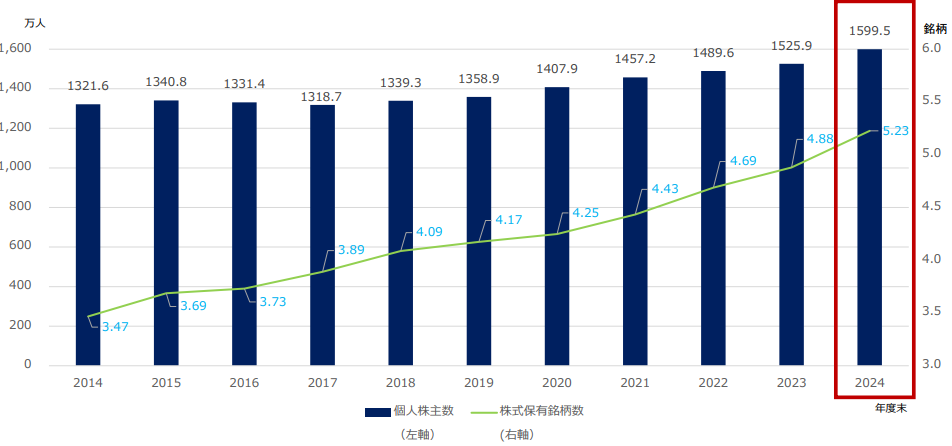
\includegraphics[width=\textwidth]{figures/figure1_1.png}
\caption{個人株主数の推移と平均保有銘柄数}
\label{fig:1.1a}
\end{subfigure}
\hfill
\begin{subfigure}{0.9\textwidth}
\centering
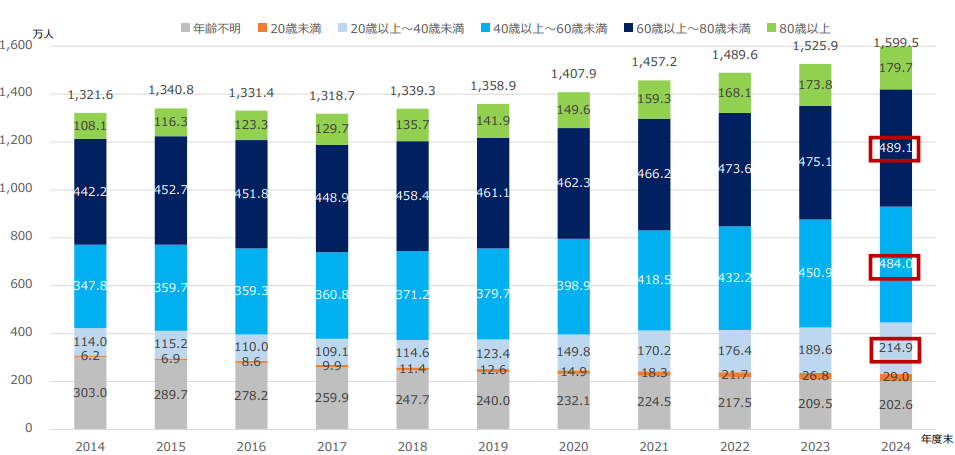
\includegraphics[width=\textwidth]{figures/figure1_2.png}
\caption{個人株主数の推移と年齢別割合}
\label{fig:1.1b}
\end{subfigure}
\caption{個人株主数の推移の平均保有銘柄数(a)と年齢別割合(b)（日本証券業協会による図,\\データ：・日本取引所グループ「株式分布状況調査」\cite{cite:3}\\・証券保管振替機構「株式等振替制度\\ 株式5,7 属性別株主数状況（人数）【6か月累計】」\cite{cite:4}）}
\label{fig:1.1}
\end{figure}


\subsection{研究目的}
本研究の目的は、金融市場における暴落現象に対し、統計力学 (RMT) と古典力学 (調和振動子) という異なる物理的アプローチを適用し、それぞれの有効性を検証すると同時に、それらを機械学習によって統合した新たな予測フレームワークを構築することである。

具体的には、TOPIX100 構成銘柄を対象とし、以下の三点を検証の柱とする。

\begin{enumerate}
    \item \textbf{RMT による同期現象の検出 (タイミングの視点):} \\
    相関行列の固有値解析を用い、市場全体の「同期 (Synchronization)」を定量化する。暴落直前に観測される秩序化 (強相関への遷移) が、システマティック・リスクの先行指標として単独で機能するかを検証する。

    \item \textbf{調和振動子モデルによる市場ポテンシャルの評価 (規模の視点):} \\
    市場価格が平衡点から乖離するほど系に歪みが蓄積されるという調和振動子モデルに基づき、市場の「ポテンシャル (Potential)」を定量化する。従来の収益率 (速度) のみに基づく指標とは異なり、この指標が市場に内在する歪みや、暴落発生時の規模 (マグニチュード) を独立して説明できるかを検証する。

    \item \textbf{機械学習による統合と実証:} \\
    上記2つの独立した物理指標を入力特徴量として LightGBM に統合し、実際の暴落事例 (COVID-19、植田ショック等) を用いたウォークフォワード検証を行う。物理法則に基づく特徴量が、ブラックボックスになりがちな機械学習モデルに対し、高い予測精度と解釈性を与えることを実証する。
\end{enumerate}

以上の取り組みを通じ、データ駆動型の機械学習と、理論主導型の物理モデルを融合させ、実務における頑健性を備えた次世代のリスク管理手法を確立することを目指す。

\clearpage
\section{伝統的経済学と経済物理学}
\subsection{伝統的経済学とその限界}
本研究で用いる経済物理学的アプローチの妥当性を論じるにあたり、まず伝統的な金融経済学の基礎となる諸仮説とその工学的観点からの限界について述べる。

\subsubsection{効率的市場仮説とランダムウォーク}
伝統的金融理論の根幹をなす「効率的市場仮説 (Efficient Market Hypothesis; EMH)」は、市場の全ての情報が即座に価格に反映されると仮定する \cite{cite:5}\cite{cite:6}。
このとき、価格の変化 (収益率) は互いに独立な確率変数となり、その推移は「ランダムウォーク」として記述される。
これは物理システムに照らせば、緩和時間が無限小であり、系の記憶が瞬時に消失するマルコフ的な極限状態を仮定していることに相当する。
現実の複雑な相互作用が存在する系において、このような相関の完全な消失を前提とするモデルは、極めて限定的な理想化であると言える。
    
\subsubsection{幾何ブラウン運動と正規分布の限界}
伝統的な金融モデルの多くは、価格変動の確率分布として「正規分布 (ガウス分布)」を前提としている \cite{cite:7}。
例えば、ブラック・ショールズモデル (Black-Scholes Model) は、株価 $S_t$ の確率的挙動を以下の確率微分方程式で記述する。

$$dS_{t}=\mu S_{t}dt+\sigma S_{t}dW_{t}$$

ここで、$W_t$ はウィーナー過程である。伊藤の補題を用いることで、対数収益率 $d(\ln S_t)$ が正規分布に従うことが導かれる。
正規分布は中心極限定理に基づき、独立した多数の事象の総和として自然界に広く観察される。
しかし、この分布の確率密度関数は $\exp(-x^2)$ で急激に減衰するため、平均から標準偏差の数倍 ($>6\sigma$) 離れた事象が発生する確率は、天文学的に低くなる。これを「薄い裾 (Thin Tail)」と呼ぶ。
現実には、ブラックマンデー (1987年) のような20\%を超える下落は、ガウス分布の世界では宇宙の年齢を待っても起こり得ない確率であるが、現実には数十年単位で発生している。

さらに、これらの伝統的モデルには、物理学的な「エネルギー保存」の観点からの欠落がある。幾何ブラウン運動は、価格の「変化率（速度）」のみをモデル化しており、
価格の「絶対水準（位置）」が持つポテンシャルエネルギーを考慮していない。これは、振り子の運動において速度（運動エネルギー）のみを観測し、
位置エネルギー（高さ）を無視することに等しく、静的な高値圏からの崩壊リスクを過小評価する要因となる。



\subsubsection{ファットテールとべき乗則}
伝統的な金融モデルが前提とするガウス分布（正規分布）の確率密度関数 $f(x)$ は次式で定義される。
\begin{equation}
f(x) = \frac{1}{\sigma\sqrt{2\pi}} \exp\left( -\frac{(x-\mu)^2}{2\sigma^2} \right)
\end{equation}
この式の核心は指数項 $\exp(-x^2)$ にある。図 2.1 (a) の黒破線が示す通り、ガウス分布は平均から離れるにつれて、その距離の2乗のオーダーで確率が急激に低下する。
これを両対数グラフで示したものが 図 2.1 (b) である。ガウス分布（黒破線）は直線にはならず、下方へ急激に曲落するカーブを描く。
これは、ガウス分布が「べき乗則」を一切持たず、極端なゆらぎを統計的に排除していることを数学的に証明している。

一方で、市場の相互作用を反映した分布として、物理学ではレヴィ安定分布が導入される\cite{mandelbrot}。
その特性関数は安定指数 $\alpha$ を用いて $\exp(-|t|^\alpha)$ と記述され、分布の裾野（テール）において累積分布関数 $P(>x)$ は以下のべき乗則に従う。
\begin{equation}
P(>x) \propto x^{-\alpha}
\end{equation}
ここで、以下の3つの領域の対比が重要となる。
    \begin{itemize}
        \item ガウス分布 ($\alpha \to \infty$)：裾が最も薄く、極端なリスクを想定しない。
        \item 厳密なレヴィ安定分布 ($0 < \alpha < 2$)：図の赤点線。べき乗則に従うが、減衰が緩やかすぎるため、分散が無限大に発散する。これは物理系としては制御不能なほど不安定な状態を指す。
        \item 実証的な逆三乗則 ($\alpha \approx 3$)：図の青実線。実際の市場データでは $\alpha \approx 3$ が観測される。ガウス分布のような指数減衰ではないため「べき乗則（直線）」に従うが、傾きが急であるため「分散は有限」に留まる。
    \end{itemize}
正規分布において、$6\sigma$ を超えるイベントが発生する確率は約 $2 \times 10^{-9}$ であり、これは確率的には「5億取引日に1回（約130万年に1回）」という、天文学的に低い頻度である。
しかし、現実の市場では、図2.1(a) の青線が示すように裾野が厚く、実証的には $6\sigma$ クラスの変動は数年に一度程度の頻度（$P \approx 10^{-3}$ オーダー）で観測される\cite{cite:9}。

図 2.1 (b) において、青色の線が対数スケールで直線になっていることが、本研究で重視する「べき乗則」の視覚的証拠である。
「べき乗則に従う」とは、数理的には式(3)の両辺の対数を取った $\log P(>x) \propto -\alpha \log x$ という線形関係を意味する。この直線性が維持される限り、どんなに巨大な $x$（暴落）であっても、
ガウス分布のように確率が消失することはなく、一定の頻度で発生し続ける。
これは市場が「分散が定義できる程度には秩序を保ちつつも、ガウス統計の枠組みでは捉えきれない破壊的なゆらぎを内包している」という、
非平衡系特有の危ういバランスの上に成り立っていることを示している。

\begin{figure}[H]
\centering
\begin{subfigure}{0.95\textwidth}
\centering
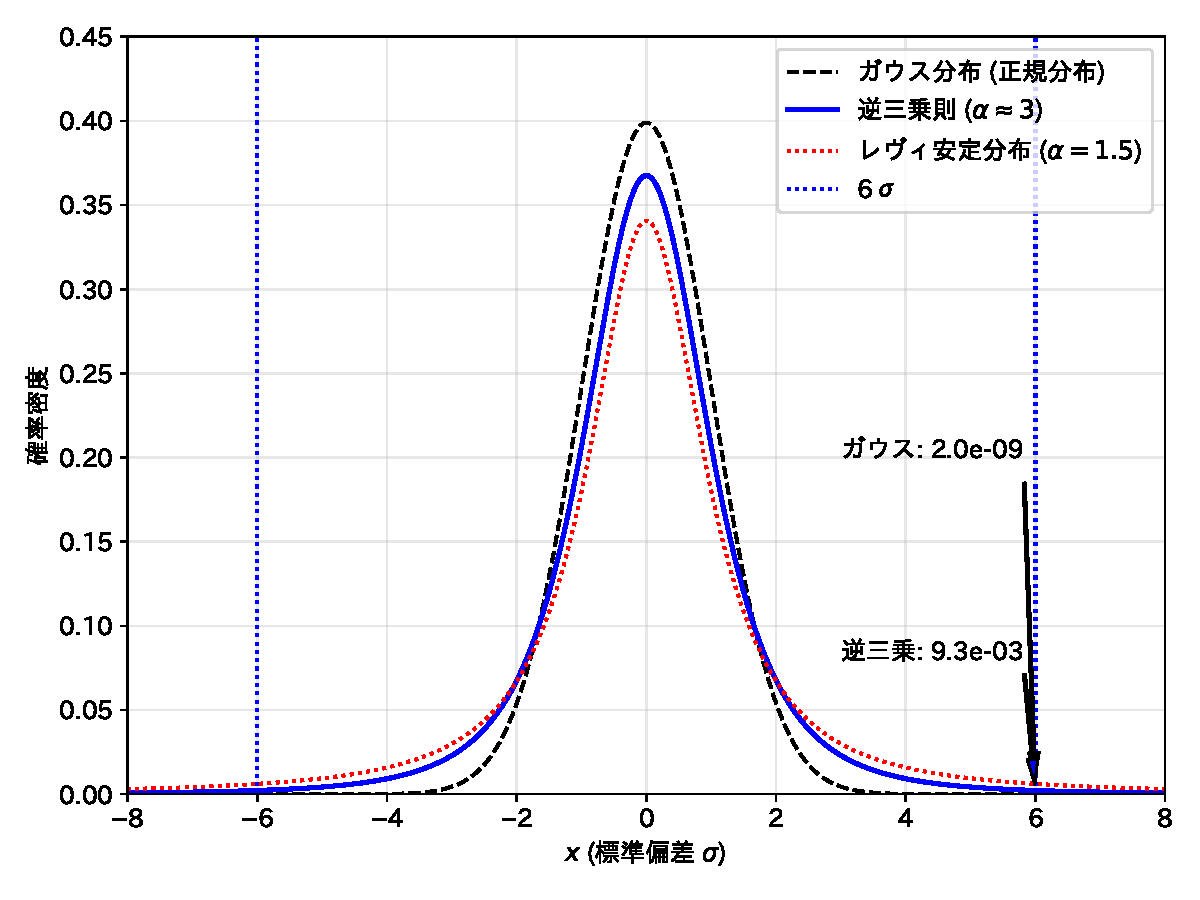
\includegraphics[width=\textwidth]{figures/fig_2_1a.pdf}
\caption{確率密度関数の比較 - 線形スケール}
\label{fig:2.1a}
\end{subfigure}
\hfill
\begin{subfigure}{0.95\textwidth}
\centering
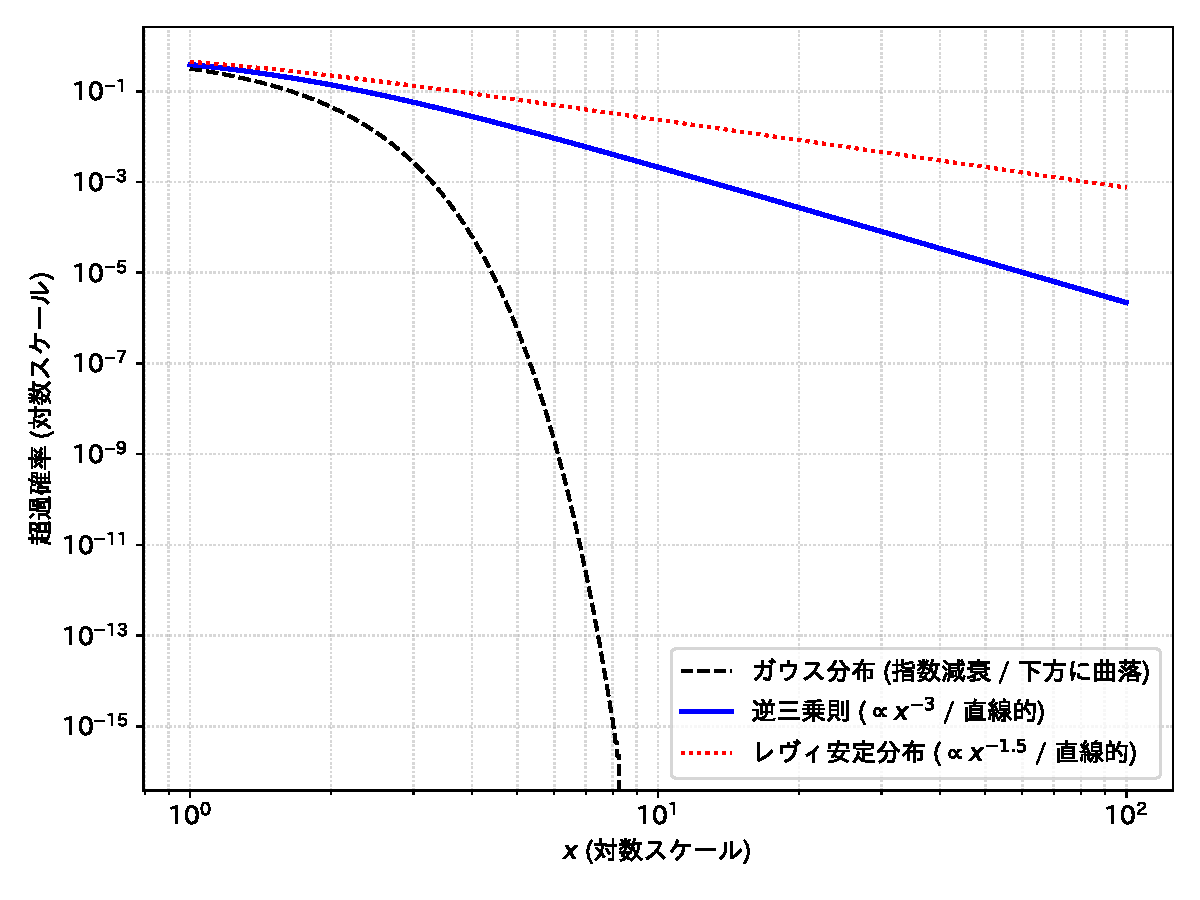
\includegraphics[width=\textwidth]{figures/fig_2_1b.pdf}
\caption{裾の確率の両対数プロット - べき乗則の証明}
\label{fig:2.1b}
\end{subfigure}
\caption{確率密度関数と裾の確率の比較}
\label{fig:2.1}
\end{figure}

\subsubsection{限定合理性と複雑系としての市場}

さらに、伝統的経済学は「ホモ・エコノミクス（完全合理的な人間）」を仮定するが、現実には投資家の「認知限界」や、他者の行動を模倣する「群集心理」が存在する。
つまり、個々の要素の単純な総和では説明できない「集団的挙動（Collective Behavior）」
が市場には内在している。具体的には、「ボラティリティ・クラスタリング」とよばれる現象である。
これは、「大きな価格変動の後には大きな変動が続き、小さな変動の後には小さな変動が続く」という現象であり、
収益率の絶対値 $|r_t|$ や二乗 $r_t^2$ に長期記憶（Long Memory）が存在することを意味する。
\begin{equation}Corr(|r_t|, |r_{t+\tau}|) > 0 \quad (\text{for large } \tau)\end{equation}
この現象は、市場参加者（エージェント）が互いに独立して行動しているのではなく、過去の価格変動や他者の行動に影響を受けていることを示唆している。
すなわち、系の中に「相互作用（Interaction）」が存在する。この相互作用こそが、統計力学における強磁性体のモデルであるイジングモデルを金融市場に応用する最大の根拠となる。
ブラック・ショールズモデルのような伝統的モデルは、外部からのニュース（外場）のみが価格を動かすと仮定しがちだが、
実際の暴落には、明確なニュースがない中で、市場内部の相互作用の連鎖（雪崩現象）によって引き起こされることがある。
Sornette\cite{cite:10}らはこれを「内在的クラッシュ（Endogenous Crash）」と呼び、外在的ショック（Exogenous Shock）と区別した。

また、これらの伝統的モデルは、価格の「変化率（速度）」の分布のみに注目し、価格の「絶対水準（位置）」が持つポテンシャルエネルギーを考慮していないという欠落がある。これは、静的な高値圏からの崩壊リスクを過小評価する要因となる。



\subsection{イジングモデルによる市場の記述と相転移}
金融市場における暴落現象を、多数の要素が相互作用を通じてマクロな秩序を形成する「相転移」として捉えるため、
統計力学の代表的なモデルであるイジングモデル（Ising Model）とのアナロジーを導入する。


\subsubsection{イジングモデルの定義とハミルトニアン}
本研究では、先行研究\cite{cite:11}や\cite{cite:12}と同様に金融市場を巨大な熱浴（外部環境）と接触し、エネルギーのやり取りを行う閉じた系と見なす。統計力学において、このような系は正準集団（Canonical Ensemble）によって記述される。
系を構成する $N$ 個の要素（スピン）の状態を $s_i \in \{+1, -1\}$ とし、系の微視的状態 (Microstate) をベクトル $\mathbf{s}=\{s_1, s_2, ..., s_N\}$ で表す。このとき、系の全エネルギーを与えるハミルトニアン $\mathcal{H}(\mathbf{s})$ は次式で定義される。
\begin{equation}
\mathcal{H}(\mathbf{s}) = -\sum_{\langle i,j \rangle} J_{ij} s_i s_j - h \sum_{i=1}^{N} s_i
\end{equation}
ここで、$J_{ij}$ は相互作用係数、$h$ は外部磁場である。正準集団において、温度 $T$ の熱浴と平衡状態にある系が、特定の微視的状態をとる確率 $P(\mathbf{s})$ は、ギブス・ボルツマン因子を用いて以下のように導出される。
\begin{equation}
P(\mathbf{s}) = \frac{1}{Z} \exp(-\beta \mathcal{H}(\mathbf{s}))
\end{equation}
ただし、$\beta$ は逆温度であり、ボルツマン定数 $k_B$ を用いて $\beta \equiv \frac{1}{k_B T}$ と定義される。ここで導入された正規化定数 $Z$ は分配関数 (Partition Function) と呼ばれ、取り得る全ての微視的状態に関する和として定義される。
\begin{equation}
Z(T, h, \{J_{ij}\}) = \sum_{\{\mathbf{s}\}} \exp(-\beta \mathcal{H}(\mathbf{s}))
\end{equation}
系が平衡状態にあるとき、自然界は自由エネルギー $F = -k_B T \ln Z$ を最小化するように振る舞う。したがって、市場の「安定状態」や「相転移」を議論することは、数学的にはこの分配関数 $Z$ の解析的性質を調べることに帰着される。る。


\subsubsection{相転移と臨界現象}
分配関数 $Z$ の厳密解を求めることは困難であるため、各スピンが隣接スピンから受ける影響を平均化された「有効磁場」として扱う平均場近似 (Mean Field Approximation) を用いる。
注目スピン $s_i$ に作用する有効磁場を $h_{eff} = zJm + h$ （$z$は配位数、$m=\langle s \rangle$は磁化）とすると、自己無撞着方程式は以下のように導かれる。
\begin{equation}
m = \tanh(\beta(zJm + h))
\end{equation}
外部磁場がない場合 ($h=0$)、この方程式が非ゼロ解（秩序相 $m \neq 0$）を持つ条件は、原点における傾きより以下のように求まる。
\begin{equation}
\frac{d}{dm} \tanh\left(\frac{zJm}{k_B T}\right) \bigg|_{m=0} = \frac{zJ}{k_B T} > 1
\end{equation}
この条件 $k_B T < zJ$ は、系の「相互作用エネルギー ($zJ$)」が、熱的な「撹乱エネルギー ($k_B T$)」を上回ったとき、系は自発的に対称性を破り、秩序状態（強磁性相）へと転移することを意味する。

\subsubsection{金融市場とのアナロジー}
前節までの物理モデルを基に、本研究における金融市場の変数を以下のように対応付ける。

\begin{itemize}
    \item \textbf{スピン $s_i$：} 各銘柄の価格変動（上昇 +1 / 下落 -1）。
    \item \textbf{外部磁場 $h$：} 市場全体に圧力をかける外部ショック（パンデミック、政策変更等）。$h < 0$ は全銘柄への売り圧力に相当する。
    \item \textbf{相互作用 $J_{ij}$：} 投資家間の模倣行動やアルゴリズム取引による同調圧力。
    \item \textbf{温度 $T$：} 市場のノイズレベル（ミクロなボラティリティ）。個々の投資家がファンダメンタルズや個別の事情に基づいてバラバラに売買を行う度合いを表す。
\end{itemize}

\textbf{(1) RMT による秩序変数 ($m^2$) の観測} \\
物理学における相転移の度合いは磁化 $m$ によって測られるが、市場データから直接 $m$ を観測することは難しい。そこで本研究では、ランダム行列理論 (RMT) の最大固有値 $\lambda_{max}$ を代替指標として用いる。
もし全銘柄が同期して動く（$s_i \approx m$）ならば、相関行列の成分は $C_{ij} \approx m^2$ となり、その最大固有値は $\lambda_{max} \approx N m^2$ となることが知られている。
すなわち、$\lambda_{max}$ の増大は、市場内部で相互作用 $J$ がノイズ $T$ を凌駕し、秩序変数 $m$ が成長していること（同期現象の進行）を数学的に等価に示すものである。

\textbf{(2) 静的な「予言」から動的な「早期検知」へ} \\
本研究では、この相転移のメカニズムを、静的な臨界点予測ではなく、外部ショック $h$ に対する「過渡応答 (Transient Response)」の監視へと応用する。
ショック発生直後、局所的な売りが相互作用 $J$ を介して系全体へ伝播し、マクロな秩序（大暴落）が形成されるまでには時間的ラグが存在する。
本研究は、RMTを用いてこの「同期の開始（$\lambda_{max}$ の急上昇）」をリアルタイムで検知し、致命的な崩壊（Avalanche）に至る前にアラートを発する「早期警戒システム」の構築を目指す。

\subsection{ランダム行列理論}
前節で述べたように、金融市場における暴落は、多数の銘柄が相互作用によって同期する「相転移現象」として理解できる。しかし、実際の価格データには個別のニュースや投機的な売買による膨大なノイズが含まれており、生のデータから市場の「秩序変数」を直接観測することは困難である。そこで本研究では、原子核物理学において複雑なハミルトニアンの統計的性質を記述するために発展し、複雑系科学に応用されているランダム行列理論 (Random Matrix Theory; RMT) を導入する [13, 14]。

\subsubsection{相関行列の構築と統計的性質}
市場内部の相関構造を抽出するため、まず観測データから経験的な相関行列 (Empirical Correlation Matrix) を構築する手順を定義する。
分析対象となる $N$ 個の銘柄について、時刻 $t$ における価格を $P_{i}(t)$ とする。金融時系列解析において価格そのものは非定常であるため、対数収益率 $R_{i}(t)$ を用いる。
\begin{equation}
R_{i}(t) = \ln P_{i}(t) - \ln P_{i}(t-1)
\end{equation}
次に、銘柄ごとに異なるボラティリティの影響を排除するため、特定の時間窓 $W$ において平均 $\mu_{i}$ および標準偏差 $\sigma_{i}$ を用いて局所的な標準化を行う。
\begin{equation}
x_{i}(t) = \frac{R_{i}(t) - \mu_{i}}{\sigma_{i}}
\end{equation}
この正規化された変数 $x_{i}(t)$ は、期間 $W$ において平均0、分散1の分布に従う。これを用いて、$N \times N$ の相関行列 $C$ の各成分 $C_{ij}$ を次のように算出する。
\begin{equation}
C_{ij} = \frac{1}{W} \sum_{\tau=1}^{W} x_{i}(t-\tau) x_{j}(t-\tau)
\end{equation}
行列形式で $\mathbf{X}$ を $N \times W$ のデータ行列（各行が銘柄、各列が時刻）とすれば、相関行列は $C = \frac{1}{W} \mathbf{X}\mathbf{X}^{T}$ と書ける。$C$ は定義より実対称行列であるため、$N$ 個の実固有値 $\lambda_{1} \le \lambda_{2} \le \cdots \le \lambda_{N}$ と、互いに直交する固有ベクトル $\mathbf{v}_{k}$ を持つ。

\subsubsection{マルチェンコ・パスツール分布}
RMTの核心は、「市場に有意な相関が全く存在しない（純粋なノイズである）」という帰無仮説を設定し、観測された固有値分布と比較することにある。
もし各銘柄の価格変動が完全に独立でランダムなガウス過程に従うと仮定した場合、その相関行列はウィシャート行列 (Wishart Matrix) と呼ばれるランダム行列のクラスに属する。
数学者マルチェンコとパスツールは、行列サイズ $N$ とデータ長 $W$ が共に無限大 ($N, W \to \infty$) であり、その比 $Q = W/N \ge 1$ が一定に保たれる極限において、固有値密度関数 $\rho(\lambda)$ が以下の解析解に収束することを証明した。

\begin{equation}
\rho_{MP}(\lambda) = \frac{Q}{2\pi\sigma^2} \frac{\sqrt{(\lambda_{+} - \lambda)(\lambda - \lambda_{-})}}{\lambda} \quad (\text{for } \lambda_{-} \le \lambda \le \lambda_{+})
\end{equation}

ここで、理論的な固有値の存在範囲を示す境界値 $\lambda_{\pm}$ は次式で与えられる（標準化データでは $\sigma^2=1$）。
\begin{equation}
\lambda_{\pm} = \sigma^{2} \left( 1 \pm \sqrt{\frac{1}{Q}} \right)^{2}
\end{equation}

この $\rho_{MP}(\lambda)$ はマルチェンコ・パスツール (Marchenko-Pastur) 分布と呼ばれ、相関行列における「熱雑音」のスペクトル特性を記述する。実際の市場データから得られた固有値のうち、範囲 $[\lambda_{-}, \lambda_{+}]$ に収まるものは、統計的なゆらぎ（ノイズ）であると判定される。

\subsubsection{最大固有値と市場の同期性}
一方、理論的上限 $\lambda_{+}$ を明確に超えて観測される固有値（逸脱固有値）は、ランダムネスでは説明できない「真の相関」を表している。本研究では、スペクトルの中で最大の値を持つ最大固有値 $\lambda_{max}$ に着目する。

\textbf{(1) マーケット・モードとしての物理的意味} \\
最大固有値 $\lambda_{max}$ は、全銘柄の価格変動に共通して含まれる成分、すなわち「マーケット・モード (Market Mode)」の強度を表す。
これに対応する固有ベクトル $\mathbf{v}^{(max)}$ の各成分 $v_{i}^{(max)}$ を調べると、通常、ほぼ全ての銘柄において同符号（正）となることが知られている。
これは、全銘柄が一斉に同じ方向（下落または上昇）へ動く「集団運動」に対応しており、前節のイジングモデルにおける「全スピンが揃った状態（秩序相）」と物理的に等価である。

\textbf{(2) 診断指標としての有効性} \\
通常時（無秩序相）において、$\lambda_{max}$ は一定の範囲内で推移する。しかし、外部ショック等により系が臨界状態に近づくと、投資家間の相互作用により売りが連鎖し、全銘柄の同期（$v_{i}^{(max)}$ の整列）が急速に進む。
これに伴い、$\lambda_{max}$ はノイズ領域 $[\lambda_{-}, \lambda_{+}]$ からさらに大きく乖離して増大する。
本研究では、この $\lambda_{max}$ の値を「相転移の進行度」を示す順序変数（Order Parameter）として監視し、市場がクラッシュの体制に入ったことを検知する主要な入力特徴量として利用する。

\subsection{調和振動子モデルと経済学}
本節では、本研究が導入する「物理的エネルギー指標（規模の視点）」の理論的背景として、古典力学における調和振動子モデルと、それを金融市場へ拡張する際の工学的近似について述べる。

\subsubsection{既存研究における市場の振動現象と証拠}
そもそも、複雑でランダムに見える金融市場を、物理学の「振動子（振り子やバネ）」として捉えることには妥当性があるのだろうか。経済に馴染みのない読者のために、まずは直感的なアナロジーから説明する。

市場価格が適正価格から大きく乖離したとき、そこには必ず価格を元に戻そうとする力が働く。これを金融用語では「平均回帰性 (Mean Reversion)」と呼ぶが、物理学の視点で見れば、これはバネが伸びきった時に重りに働く「復元力 ($F=-kx$)」そのものである。もし市場にこのような復元力が全くなければ、価格は一度離れたら二度と戻ってこない（発散する）ことになるが、現実の市場は常に一定の範囲内で変動を続けている。この「行き過ぎたら戻る」という反復運動の存在自体が、市場が本質的に振動子システムであることを示唆している。

この直感を裏付ける定量的な証拠も、近年の経済物理学の研究によって示されている。
例えば、Ye \& Huang (2008) \cite{ye2008non} は、従来の古典的なモデルでは説明できない市場の持続的な変動を、量子力学的な振動子モデルを用いることで説明できることを示した。
また、Ahn et al. (2017) \cite{ahn2017modeling} は、量子調和振動子 (Quantum Harmonic Oscillator; QHO) モデルを実際の市場データ（FTSE All-Share Index等）に適用し、従来の金融工学モデル（幾何ブラウン運動など）よりも圧倒的に高い精度で市場の確率分布を再現できることを実証した。特に、彼らの研究は、市場データに見られる「極端な変動（ファットテール）」が、調和振動子の「励起状態（エネルギーが高い状態）」として数学的に記述できることを明らかにした。

これらの先行研究は、市場には目に見えない「ポテンシャル（器）」が存在し、株価という粒子がその中で振動運動を行っているという物理モデルが、単なる比喩ではなく、数理的にも極めて有効であることを証明している。本研究は、この確立された振動子モデルの概念を、暴落規模の予測へと応用するものである。

\subsubsection{物理学における調和振動子とエネルギー}
調和振動子 (Harmonic Oscillator) は、平衡点からの変位に比例する復元力が働く系であり、物理学において最も基礎的かつ重要なモデルの一つである。
バネ定数 $k$ のバネに繋がれた粒子が一次元上を運動している場合、平衡点からの変位を $x$ とすると、系に蓄えられるポテンシャルエネルギー (位置エネルギー) $U$ は次式で定義される。
\begin{equation}
U(x) = \int_{0}^{x} kx' dx' = \frac{1}{2}kx^{2}
\end{equation}
この式は、「系が平衡状態から大きく乖離する ($|x|$ が大きくなる) ほど、その二乗に比例して系内部に蓄積されるエネルギーは増大する」という法則を示している。
また、系の全エネルギー（ハミルトニアン） $\mathcal{H}$ は、運動エネルギー $K$ とポテンシャルエネルギー $U$ の和として保存される（保存系の場合）。
\begin{equation}
\mathcal{H} = K + U = \frac{p^{2}}{2m} + \frac{1}{2}kx^{2}
\end{equation}
ここで $p$ は運動量、$m$ は質量である。この物理法則は、エネルギーが「運動（速度）」と「位置（変位）」の二つの形態を行き来することを示唆している。




\subsection{市場ポテンシャル指標}
\subsubsection{金融市場への適用と変数の定義}
経済物理学の分野において、価格変動を振動現象として捉える試みは存在するが、本研究ではこれを「リスクのポテンシャル評価」に特化して適用する。
市場における物理変数を以下のように定義する。

\begin{itemize}
    \item \textbf{変位 $x(t)$：} 株価 $P(t)$ そのもの。
    \item \textbf{バネ定数 $k$：} 発行済株式数 $S$。その銘柄が市場全体に対して持つ「慣性」や「重み」を表す係数とする。
\end{itemize}

この定義に基づくと、ある銘柄 $i$ が持つポテンシャルエネルギー $U_i(t)$ は次のように記述される。
\begin{equation}
U_i(t) \propto S_i \cdot P_i(t)^2 = M_i(t) \cdot P_i(t)
\end{equation}
ここで $M_i(t) = S_i \cdot P_i(t)$ は時価総額である。すなわち、市場ポテンシャルは「時価総額に、さらに株価水準 $P_i$ による重み付けを行った物理量」として解釈される。
これは、同じ時価総額の企業であっても、低位株（$P$小）より高位株（$P$大）の方が、崩落時の変動幅（値幅）が大きいため、系に与える物理的衝撃（エネルギー解放量）が大きいという市場特性を反映している。

\subsubsection{運動エネルギーとポテンシャルエネルギーの相補性}
本研究が、従来のボラティリティ指標（運動エネルギー）に加えて、このポテンシャル指標（位置エネルギー）を導入する最大の理由は、リスク評価の完全性にある。
式(10)のハミルトニアンが示す通り、物理系の状態は片方だけでは記述できない。

\begin{itemize}
    \item \textbf{運動項 $K$（ボラティリティ）大：} 既に価格が激しく動いている状態（暴落中）。従来モデルでも検知可能。
    \item \textbf{ポテンシャル項 $U$（価格水準）大：} 嵐の前の静けさ。速度はゼロだが、系は巨大な位置エネルギーを蓄積している。
\end{itemize}

従来の金融モデルは後者の「静的な高エネルギー状態」を見落とす傾向がある。本研究で導入する $P^2$ 指標は、この「見えない位置エネルギー」を定量化し、運動エネルギーと合わせて監視することで、市場の全リスク量を包括的に記述しようとする試みである。

\subsubsection{平衡点設定に関する物理的解釈}
本モデルの構築にあたり、調和振動子の平衡点（変位 $x=0$）を、移動平均等の相対値ではなく、原点 ($P=0$) に設定する本研究独自の仮説について議論する。
通常、経済学では理論価格からの乖離を重視する。しかし、本研究の目的は、システム全体が機能不全に陥るような「致命的な相転移（暴落）」における最大リスクの評価である。

物理学のアナロジーにおいて、物体が持つ位置エネルギーは、基準面（グラウンド・レベル）からの絶対的な高さによって規定される。市場における「グラウンド・レベル」とは、株価が価値を失う地点、すなわち $P=0$（倒産・無価値）である。
したがって、本研究では「株価の上昇は、それ自体が系をより高いエネルギー準位（励起状態）へと持ち上げる行為であり、潜在的な落下エネルギーを蓄積させる」と解釈する。
この仮定に基づけば、移動平均からの乖離が小さくとも、絶対的な価格水準が高い銘柄は、ひとたび相転移が発生した際に解放しうるエネルギー量が巨大である（高所からの落下に相当する）と評価できる。
この設定は、平常時の微小振動を記述するモデルとしては粗いが、本研究が対象とする「システマティック・リスクの規模評価」という限定された局面においては、リスクを保守的（最大値）に見積もるための有効な代理変数 (Proxy) として機能する。


\clearpage
\section{金融市場と機械学習}
本章では、前章で定義した物理的特徴量（RMT 指標など）を入力とし、将来の市場変動を予測するための数学的フレームワークとして、機械学習の理論的基礎とその適用について述べる。

\subsection{機械学習の数理的定式化}
機械学習 (Machine Learning) とは、工学的にはデータから規則性を抽出するアルゴリズムの総称であるが、物理学的な視点では、未知の確率分布 $P(X,Y)$ から生成された有限の標本集合 $\mathcal{D}=\{(x_{i},y_{i})\}_{i=1}^{N}$ に基づき、入力から出力 $y$ を写像する関数 $f:X\rightarrow Y$ を、汎化誤差 (Generalization Error) を最小化するように決定する「変分原理に基づく最適化問題」として定式化される。

\subsubsection{経験リスク最小化と正則化}
真の分布 $P(X,Y)$ が未知である以上、期待リスク（真の誤差）を直接計算することは不可能である。そのため、学習は以下の経験リスク $R_{emp}(f)$ を最小化する関数 $f$ を仮説空間 $\mathcal{H}$ から探索する過程に帰着される。
\begin{equation}
R_{emp}(f) = \frac{1}{N} \sum_{i=1}^{N} L(y_{i}, f(x_{i}))
\end{equation}
ここで、$L(y, \hat{y})$ は損失関数 (Loss Function) であり、予測値と真値の乖離による「エネルギー」を定義する。
しかし、有限のデータに対して $R_{emp}$ を過度に最小化すると、ノイズまで学習してしまう過学習 (Overfitting) が発生する。これを防ぐため、物理学におけるラグランジュの未定乗数法と同様に、関数の複雑さにペナルティを課す正則化項 $\Omega(f)$ を加えた構造リスク $R_{reg}(f)$ の最小化を行う。
\begin{equation}
\hat{f} = \mathop{\rm argmin}_{f \in \mathcal{H}} \left( R_{emp}(f) + \lambda \Omega(f) \right)
\end{equation}
この $f$ を求めるプロセスは、統計力学における自由エネルギー $F = E - TS$ の最小化（エネルギー最小化とエントロピー最大化の競合）と数理的に等価な構造を持つ。

\subsection{勾配ブースティング決定木と LightGBM}
金融時系列データのような、高次元かつ非線形性が強いテーブルデータに対して、現在最も高い予測精度を示す手法の一つが勾配ブースティング決定木 (Gradient Boosting Decision Tree; GBDT) である。本研究では、その高速かつ高精度な実装である LightGBM を採用する。

\subsubsection{関数空間における勾配降下法}
勾配ブースティングは、単一の予測モデルを作るのではなく、複数の「弱学習器 (Weak Learner)」 $h_{m}(x)$ の線形結合によって、最終的な強学習器 $F_{M}(x)$ を構成するアンサンブル学習手法である。
\begin{equation}
F_{M}(x) = \sum_{m=1}^{M} \gamma_{m} h_{m}(x)
\end{equation}
このモデル構築過程は、関数空間における勾配降下法として解釈できる。第 $m$ ステップにおいて、現在のモデル $F_{m-1}(x)$ の残差（損失関数の負の勾配）を近似するように新たな学習器 $h_{m}(x)$ を追加する。
\begin{equation}
h_{m}(x) \approx - \left[ \frac{\partial L(y, F(x))}{\partial F(x)} \right]_{F(x)=F_{m-1}(x)}
\end{equation}
これは、物理シミュレーションにおける摂動展開や、ポテンシャルの谷底へ向かって徐々に補正項を加えていく反復解法と同様のアルゴリズムである。

\subsubsection{LightGBM の採用理由と物理的適合性}
近年、金融工学の分野においても LSTM や Transformer といった深層学習 (Deep Learning) の応用が進んでいる。しかし、本研究では以下の物理的・工学的理由から、あえて決定木ベースの LightGBM をソルバーとして採用する。

\begin{itemize}
    \item \textbf{特徴空間における「時間」の凝縮：}
    深層学習（RNN系列）の強みは、モデル内部で時系列の長期記憶を保持できる点にある。しかし本研究では、第2章で定義した通り、RMT（過去 $W$ 日間の相関構造）や調和振動子（蓄積されたポテンシャル）といった「特徴量」そのものに、時間的な履歴情報や力学的な状態が集約されている。
    したがって、予測器に求められる役割は、複雑な時系列パターンの抽出ではなく、入力された物理的状態変数（State Variables）から崩壊リスクへの「非線形写像」を正確に行うことである。このタスクにおいては、決定木アンサンブルが極めて高い効率を示す。

    \item \textbf{異質な物理量の統合能力：}
    本モデルへの入力には、固有値（無次元量）、エネルギー（価格の二乗オーダー）、収益率（パーセント）といった、物理的次元やスケールが全く異なる変数が混在する。
    決定木は特徴空間を直交する超平面で分割するため、入力変数のスケーリングや分布形状（正規分布か否か）に依存せず、ロバストに学習が可能である。

    \item \textbf{低S/N比環境での汎化性能：}
    金融市場はシグナルに対してノイズが極めて多い系である。パラメータ数が膨大な深層学習モデルは、十分なデータ量が確保できない場合、ノイズパターンを過剰に記憶（過学習）するリスクが高い。対して、多数の弱学習器のアンサンブルである LightGBM は、統計的に分散を抑制する効果が強く、限られた暴落サンプル数でも安定した汎化性能を発揮する。
\end{itemize}


\subsection{不均衡データ学習と評価指標}
金融市場における暴落予測は、機械学習の分類問題として定式化できるが、一般的な画像認識などとは異なる「クラスの不均衡性 (Class Imbalance)」という大きな課題を抱えている。

\subsubsection{混同行列と不均衡性の壁}
市場データの99\%以上は「平時（暴落なし）」であり、「暴落」は数年に一度の希少事象（レアケース）である。このような状況下では、モデルが「常に異常なし」と予測するだけで、見かけ上の正解率 (Accuracy) は99\%を超えてしまう。しかし、リスク管理において最も重要なのは、その残り1\%未満の暴落を確実に捉えることである。
したがって、単なる正解率ではなく、予測結果と真の結果の組み合わせを表す「混同行列 (Confusion Matrix)」に基づいた詳細な評価が必要となる。

\begin{itemize}
    \item \textbf{真陽性 (True Positive; TP)}：実際に暴落が発生し、モデルも正しく「暴落」と予測できた場合（成功）。
    \item \textbf{偽陽性 (False Positive; FP)}：実際には暴落しなかったが、モデルが誤って「暴落」と予測した場合（空振り）。
    \item \textbf{偽陰性 (False Negative; FN)}：実際に暴落が発生したにもかかわらず、モデルが「平時」と予測して見逃した場合（致命的な失敗）。
    \item \textbf{真陰性 (True Negative; TN)}：平時において、モデルも正しく「平時」と予測した場合。
\end{itemize}

\subsubsection{再現率 (Recall) と適合率 (Precision)}
上記に基づき、本研究では特に以下の二つの指標を重視する。

第一に\textbf{「再現率 (Recall)」}である。これは、実際に起きた全ての暴落のうち、モデルがどれだけを検知できたかを示す指標であり、リスク管理における「安全性（見逃しのなさ）」を意味する。
\begin{equation}
\text{Recall} = \frac{\text{TP}}{\text{TP} + \text{FN}}
\end{equation}
物理的な暴落（相転移）の予兆検知において、FN（見逃し）は資産の壊滅的損失を意味するため、Recallの最大化は最優先事項となる。

第二に\textbf{「適合率 (Precision)」}である。これは、モデルが発したアラートのうち、実際に暴落に結びついた割合を示し、システムの「信頼性」を意味する。
\begin{equation}
\text{Precision} = \frac{\text{TP}}{\text{TP} + \text{FP}}
\end{equation}
Recall を高めようとして判定基準を緩めると、必然的に FP（空振り）が増加し、Precision は低下する（トレードオフ関係）。実務的には、FP が多すぎるとアラートが無視される要因となるため、一定の Precision を維持しつつ Recall を最大化するバランスが求められる。
このトレードオフ関係を可視化し、モデルの性能を総合的に評価するために、横軸に Recall、縦軸に Precision をとった PR曲線 (Precision-Recall Curve) を用いる。

\subsection{モデルの解釈性とSHAP}
LightGBM のような高度な決定木アンサンブルモデルは、高い予測精度を持つ反面、内部計算が複雑化し、人間には判断根拠が理解しにくい「ブラックボックス」となりやすい。物理的アプローチを標榜する本研究において、モデルが「なぜ暴落と判断したか」を説明できないことは致命的である。
そこで本研究では、協力ゲーム理論に基づく特徴量重要度算出手法である \textbf{SHAP (SHapley Additive exPlanations)} を導入する。

\subsubsection{シャープレイ値による寄与度分解}
SHAP は、あるインスタンス（特定の日時）に対するモデルの予測値 $f(x)$ を、各特徴量の貢献度（SHAP値）の総和として分解する手法である。
ゲーム理論において、複数のプレイヤーが協力して報酬を得た際、その報酬を各プレイヤーの貢献度に応じて公正に分配する「シャープレイ値」という概念がある。SHAP はこれを機械学習に応用したものであり、
「モデルの予測値」を報酬、「入力特徴量」をプレイヤーと見なすことで、特徴量 $i$ の寄与度 $\phi_i$ を次式のように算出する。

\begin{equation}
\phi_i = \sum_{S \subseteq F \setminus \{i\}} \frac{|S|! (|F| - |S| - 1)!}{|F|!} [f_{S \cup \{i\}}(x_{S \cup \{i\}}) - f_S(x_S)]
\end{equation}

ここで、$F$ は全特徴量の集合、$S$ はその部分集合を表す。この式は、特徴量 $i$ が「有無」によって予測値をどれだけ変化させたかを、あらゆる組み合わせについて平均化したものである。
この SHAP値を用いることで、モデル全体でどの物理指標が重要であるかという「大域的解釈 (Global Interpretability)」だけでなく、特定の暴落日において何が決定打となったかという「局所的解釈 (Local Interpretability)」が可能となり、モデルの物理的妥当性を検証することができる。






\clearpage
\section{提案手法}
本章では、市場の「同期現象 (タイミング)」と「潜在エネルギー (規模)」の両面から暴落を予知する新たなフレームワークを提案する。

\subsection{解析対象とデータセット}
\subsubsection{解析対象 (Analysis Target)}
本研究では、株式会社日本取引所グループ (JPX) が提供するデータを用い、東京証券取引所における時価総額および流動性の高い上位100銘柄で構成される \textbf{TOPIX100} を解析対象とする。
TOPIX100 は、個別の仕手的な動きが少なく、市場全体のマクロな相互作用（相転移）を観測するのに適している。

データの期間は、\textbf{2016年1月30日から2026年1月15日までの約10年間}とする。
本研究では、過去のデータを用いて逐次的に未来を予測する実運用環境を模倣するため、ウォークフォワード分析 (Walk-Forward Analysis) を採用する。これにより、単一の期間だけでなく、以下の異なる市場環境下における複数の主要な暴落イベントに対して検証を行う。

\begin{itemize}
    \item \textbf{COVID-19 ショック (2020年):} 未知の感染症によるパンデミック性の暴落。
    \item \textbf{植田ショック (2024年):} 金融政策の変更（利上げ懸念）に起因する急落。
    \item \textbf{関税ショック (2025年):} 地政学的リスクと貿易摩擦によるシステマティックな暴落。
\end{itemize}

なお、株式分割等の影響については、過去に遡及して補正した調整後株価を使用し、時系列の連続性を担保している。

\subsubsection{データ前処理}
取得した生の市場データは、物理モデルへの入力とするには不適切なノイズや不連続性を含んでいる。本研究では、市場の統計的性質を正しく抽出するため、以下の手順で前処理を行った。

\begin{description}
\item[株式分割の調整]
株価は企業の資本政策（株式分割等）によって不連続に変化しうる。例えば、1株を2株に分割した場合、理論価値は変わらないにもかかわらず、株価は半値となり、時系列データとしては「50\%の暴落」として記録される。
このような非物理的なノイズを排除し、時系列の連続性を担保するため、本研究では調整係数を用いて過去の価格を遡及的に補正した「調整後株価」を使用する。
これにより、モデルは純粋な市場の需給に基づく価格変動のみを学習対象とすることが可能となる。

\item[欠損値の処理]
RMT（ランダム行列理論）による固有値解析は、行列の次元数（銘柄数 $N$）が全期間を通じて一定であることを前提とする。
そのため、データセット期間中に新規上場（IPO）または上場廃止等の理由でデータが欠損する不完全な銘柄については、解析対象から除外した。 
具体的には、ソフトバンク(2018年上場)とソニーフィナンシャルグループ(2025年上場)を削除した結果、解析対象は最終的に N=98 銘柄となった。
また、商船三井およびアシックスの2銘柄について確認された一時的な時価総額データの欠損については、当該期間における適時開示情報等を確認し、株式分割や併合等のコーポレートアクションが行われていないことを特定した。その上で、発行済株式数が一定であると見なし、取得された生株価と発行済株式数の積によって時価総額を再計算し、欠損を補完した。
\end{description}

\subsubsection{変数の定義 (Variable Definitions)}
物理モデルへの適用に先立ち、本研究で使用する基礎変数およびシステム全体の挙動を記述するマクロ指標を定義する。

\textbf{1. 基礎変数}
\begin{itemize}
    \item \textbf{株価 ($P_i(t)$):} 銘柄 $i$ の時刻 $t$ における調整後終値。物理的には振動子の「変位」に対応する。
    \item \textbf{発行済株式数 ($S_i(t)$):} 銘柄 $i$ の市場に流通している株式総数。物理的には振動子の「質量係数（バネ定数）」に対応する。
    \item \textbf{時価総額 ($M_i(t)$):} 企業の経済的価値の総量。$M_i(t) = P_i(t) \times S_i(t)$ で定義される。
\end{itemize}

\textbf{2. システム指標の定義 (Index Definition)}
本研究では、機械学習モデルの学習ターゲット（正解ラベル）を作成するために、性質の異なる以下の2つのシステム指標（インデックス）を定義する。

\begin{itemize}
    \item \textbf{インデックス1：経済指標 ($I_{eco}$)} \\
    従来の時価総額加重平均型インデックス。市場の「経済的価値の総和」を表す一般的な指標である。
    \begin{equation}
    I_{eco}(t) = \sum_{i=1}^{N} M_i(t) = \sum_{i=1}^{N} S_i(t) P_i(t)
    \end{equation}
    これは $P$ の一次式で構成され、通常のTOPIX等の動きに準拠する。
    
    \item \textbf{インデックス2：市場インパクト指標 ($I_{imp}$)} \\
    市場インパクト指標 ($I_{imp}$)
本研究が機械学習エンジニアリングの観点から導入する、暴落の「インパクト」を強調した指標である。経済指標 $I_{eco}$ を非線形変換（二乗）することで定義される。
    \begin{equation}
   I_{imp}(t) = \{ I_{eco}(t) \}^{2} = \left( \sum_{i=1}^{N} S_{i}(t) P_{i}(t) \right)^{2}
    \end{equation}
   この指標は、物理的な意味（市場全体を単一の振動子と見なした場合のポテンシャルエネルギー $\propto X^2$）を模倣しつつ、工学的には「信号増幅 (Signal Amplification)」のためのフィルタとして機能する。時価総額の総和が大きい（市場が高値圏にある）状態での変動を二乗の効果によって増幅させることで、低位における小規模なノイズを相対的に抑制し、市場全体に甚大な影響を与えるクラッシュのみを選択的に学習させることを目的とする。
\end{itemize}

\subsection{目的変数の定義と正解ラベルの作成}
教師あり学習において最も重要な「正解ラベル（何をもって暴落とするか）」の定義について述べる。
本研究では、単なる株価の下落ではなく、物理的に意味のある「相転移（暴落）の予兆」を捉えるため、正解ラベルの作成にあたり (1) 複合条件による判定、(2) インパクト強度に基づく重み付け、の二段階のプロセスを導入する。

\subsubsection{複合条件による暴落判定}
単日の下落のみを暴落と定義すると、翌日にすぐ反発するような「ノイズ（ダマシ）」を学習してしまうリスクがある。そこで本研究では、短期的な急落と中期的な下落トレンドの両方を捉えるため、以下の\textbf{複合条件}を採用する。

時刻 $t$ におけるターゲット変数を $y_t \in \{0, 1\}$ とし、向こう $k$ 日間の収益率を $R_{t+k}$ とする。以下の2つの条件を同時に満たした場合のみ、その時点 $t$ を「暴落の予兆あり ($y_t=1$)」と定義する。

\begin{equation}
y_t = 
\begin{cases} 
1 & \text{if } (R_{t+3} < x) \land (R_{t+10} < y) \\
0 & \text{otherwise}
\end{cases}
\end{equation}

ここで、\begin{equation}
R_{t+k} = \frac{I(t+k) - I(t)}{I(t)}
\end{equation}
は時刻 $t$ から $t+k$ 日後までのインデックス変化率を表す。
また、$x$ は3日後の短期下落閾値、$y$ は10日後の中期下落閾値である。

\subsubsection{物理的重み付け関数 (Sample Weighting) の定義}
不均衡データ問題（暴落データが極端に少ない問題）に対処し、かつモデルに「どの暴落が物理的に重要か」を学習させるため、正解ラベル $y_t=1$ となった各サンプルに対し、物理的強度に基づく重み $w(t)$ を付与する。
これは、機械学習における「コスト考慮型学習 (Cost-sensitive Learning)」を本研究の物理モデルに合わせて定式化したものであり、以下の数式で定義される。

\begin{equation}
w(t) = w_{base} \times \underbrace{\exp(-\gamma \cdot \Delta t)}_{\text{時間減衰項}} \times \underbrace{\frac{|R(t)|}{|\theta|}}_{\text{強度比例項}}
\end{equation}

各項の物理的・工学的意味は以下の通りである。

\begin{itemize}
    \item \textbf{時間減衰項 (Time Decay Term):} \\
    $\Delta t$ は暴落判定（相転移）が開始してからの経過日数、$\gamma$ は減衰率（本研究では $\gamma=0.5$）である。
    実務上、暴落予測において最も価値があるのは「発生直後の初動 (Nucleation)」である。発生から日が経った後のデータ（余震フェーズ）の重みを指数関数的に減衰させることで、モデルが「暴落の最中」ではなく「相転移の開始点」に焦点を合わせて学習するよう誘導する。
    
    \item \textbf{強度比例項 (Severity Term):} \\
    $R(t)$ は実際の下落率、$\theta$ は閾値である。
    ギリギリで判定基準を満たした下落よりも、基準を大きく下回る壊滅的な崩壊（-20\%など）に対して、その倍率に応じたペナルティ（重み）を与える。これにより、モデルは「小規模な調整」よりも「致命的なクラッシュ」を優先的に学習するようになる。
\end{itemize}

この重み $w(t)$ は、後述する学習プロセスにおいて損失関数 (Loss Function) の係数として直接使用される。

\subsubsection{グリッドサーチによる多段階閾値選定プロセス}
閾値の設定において、単一の指標のみで最適化を行うことは、特定のデータセットへの過学習（Data Snooping）を招くリスクがある。
そこで本研究では、全32通りのパラメータ候補に対し、統計的な「量」と物理的な「質」の観点から、以下の二段階のフィルタリングを行うことで、最もロバストな閾値を決定した。

\textbf{Step 1: 統計的分布に基づくスクリーニング (Table 4.1)} \\
第一段階では、過学習を防ぐため、極端な挙動を示すパラメータを除外した。評価指標には以下を用いた。
\begin{itemize}
    \item \textbf{Events (検知回数)}: 10年間における暴落イベントの発生回数。
    \item \textbf{Days (検知総日数)}: 暴落と判定された日数の合計。
    \item \textbf{Ratio (Events/Days)}: 1イベントあたりの平均日数の逆数。この値が高すぎる場合、単発的な下落（ノイズ）を多く拾っていることを示唆する。
\end{itemize}
分析の結果、Ratio が $0.29 \sim 0.45$ の範囲に分布する中で、極端にイベント数が多すぎる群（ノイズ過多）と、少なすぎる群（学習データ不足）を除外し、分布の中央付近に位置する16通り（Middle 16）を候補として抽出した。

\begin{table}[H]
\centering
\caption{統計的指標によるスクリーニング（抜粋）。イベント数と発生比率(Ratio)に基づき、極端な設定を除外した。}
\label{tab:grid_step1}
\small
\begin{tabular}{cccccc}
\hline
Condition (Short / Long) & Events & Days & Ratio (E/D) & Status \\
\hline
\multicolumn{5}{c}{\textit{--- Too Loose (Noise Dominant) ---}} \\
5d -2.0\% / 7d -4.0\% & 123 & 382 & 0.322 & Excluded \\
3d -2.0\% / 7d -4.0\% & 119 & 288 & 0.413 & Excluded \\
\hline
\multicolumn{5}{c}{\textit{--- Middle 16 (Robust Candidates) ---}} \\
5d -2.0\% / 10d -8.0\% & 59 & 187 & 0.316 & Candidate \\
\textbf{3d -2.0\% / 10d -8.0\%} & \textbf{55} & \textbf{153} & \textbf{0.359} & \textbf{Candidate} \\
3d -3.0\% / 10d -8.0\% & 57 & 132 & 0.432 & Candidate \\
\hline
\multicolumn{5}{c}{\textit{--- Too Strict (Data Sparse) ---}} \\
5d -3.0\% / 10d -10.0\% & 40 & 125 & 0.320 & Excluded \\
3d -2.0\% / 10d -10.0\% & 40 & 110 & 0.364 & Excluded \\
\hline
\end{tabular}
\end{table}

\textbf{Step 2: 物理的強度に基づく最終選定 (Table 4.2)} \\
第二段階では、Step 1 を通過した候補の中から、本研究の目的に合致する「システムへの影響が甚大な暴落」を捉えている設定を選定した。評価指標には以下を用いた。
\begin{itemize}
    \item \textbf{Avg\_Weight}: 検知期間中の平均インパクト強度。
    \item \textbf{Max\_Weight}: 検知期間中の最大インパクト強度。
\end{itemize}
表 4.2 に示すように、候補の中で \textbf{Avg\_Weight} および \textbf{Max\_Weight} を比較した結果、イベント数を確保しつつ（Events=55）、最も高い平均強度（Avg=5.63）を示し、かつ最大強度（Max=25.85）も十分に高い以下の条件を最適解として採用した。

\begin{equation}
\text{Target Condition: } (3\text{d} < -2.0\%) \land (10\text{d} < -8.0\%)
\end{equation}

\begin{table}[H]
\centering
\caption{物理的強度による最終選定（Middle 16からの抜粋）。学習に必要なイベント数を維持しつつ、Avg\_Weight（物理的純度）が最も高い条件を採用した。}
\label{tab:grid_step2}
\small
\begin{tabular}{cccccc}
\hline
Condition & Events & Avg\_Weight & Max\_Weight & Decision \\
\hline
5d -2.0\% / 10d -8.0\% & 59 & 4.87 & 25.85 & Not Selected (Low Avg) \\
\textbf{3d -2.0\% / 10d -8.0\%} & \textbf{55} & \textbf{5.63} & \textbf{25.85} & \textbf{Selected (Best Balance)} \\
3d -3.0\% / 10d -8.0\% & 57 & 6.27 & 25.85 & Not Selected (Unstable Ratio) \\
5d -2.0\% / 10d -6.0\% & 73 & 5.71 & 34.47 & Not Selected (Too Frequent) \\
\hline
\end{tabular}
\end{table}

この二段階のプロセスにより、単に予測しやすいデータを選ぶのではなく、統計的に安定し、かつ物理モデルの意図する「高エネルギー事象」を的確に捉えるターゲット定義を行うことができた。

\subsubsection{比較対象（インデックス1）への適用}
インデックス2はインデックス1の二乗 ($I^2$) で定義されるため、微小な変動率 $r$ において、インデックス2の変動率はインデックス1の約2倍 ($2r$) となる。したがって、比較の公平性を保つため、インデックス1の判定閾値には、インデックス2で最適化された閾値の半分の値を適用した。
\begin{equation}
\text{Target Condition: } (3\text{d} < -1.0\%) \land (10\text{d} < -4.0\%)
\end{equation}

\subsection{入力特徴量の設計}
本研究では、予測モデルへの入力として、以下の3つのカテゴリの特徴量を設計した。

\subsubsection{テクニカル特徴量 (Baseline Features)}
従来の金融工学アプローチに基づくベースラインとして、以下の標準的な指標を採用する。これらは経済空間（価格・出来高）の情報のみを利用しており、物理的アプローチを行わない場合の比較基準となる。

\begin{itemize}
    \item \textbf{対数収益率 (Log-return):} \\
    市場平均（TOPIX100）の速度成分を表す。
    \begin{equation}
        R(t) = \ln \left( \frac{P(t)}{P(t-1)} \right)
    \end{equation}

    \item \textbf{ボラティリティ (Volatility):} \\
    リスク指標として、過去20日間の対数収益率の標準偏差を採用する。
    \begin{equation}
        \sigma_{20}(t) = \sqrt{\frac{1}{20} \sum_{k=0}^{19} (R(t-k) - \overline{R})^2}
    \end{equation}

    \item \textbf{モメンタム (Momentum / ROC):} \\
    過去10日間の価格変化率（Rate of Change）であり、トレンドの慣性を測る指標である。
    \begin{equation}
        Mom_{10}(t) = \frac{P(t)}{P(t-10)} - 1.0
    \end{equation}

    \item \textbf{相対力指数 (RSI):} \\
    過去14日間における価格上昇幅と下落幅のバランスから、市場の過熱感を判定するオシレーター指標である。本研究では単純移動平均（SMA）を用いた以下の定義を採用する。
    \begin{equation}
        RSI(t) = 100 - \frac{100}{1 + RS(t)}, \quad RS(t) = \frac{\overline{Gain}_{14}(t)}{\overline{Loss}_{14}(t)}
    \end{equation}
    ここで、$\overline{Gain}_{14}$ は過去14日間の前日比プラス分の平均、$\overline{Loss}_{14}$ はマイナス分（絶対値）の平均である。
\end{itemize}

\subsubsection{RMT特徴量 (Structural Features)}
市場全体の「同期構造」を定量化するため、第2章で定義したランダム行列理論 (RMT) に基づく指標を算出する。

RMT特徴量の算出にあたっては、データの定常性を確保し、純粋な相関関係のみを取り出すため、以下の数理プロセスを経て計算を行う。

\begin{itemize}
    \item \textbf{Step 1: 運動変数の生成 (Log-return)} \\
    まず、各銘柄 $i$ の調整後株価 $P_{i}(t)$ の対数差分（対数収益率）を計算し、価格スケールに依存しない速度成分 $r_{i}(t)$ を生成する。
    \begin{equation}
        r_{i}(t) = \ln P_{i}(t) - \ln P_{i}(t-1)
    \end{equation}

    \item \textbf{Step 2: 局所的正規化 (Local Normalization)} \\
    銘柄ごとに異なるボラティリティの影響を排除するため、解析対象となる時間窓 $W$ における平均 $\mu_{i}$ および標準偏差 $\sigma_{i}$ を用いて標準化を行う。
    \begin{equation}
        \hat{r}_{i}(\tau) = \frac{r_{i}(\tau) - \mu_{i}}{\sigma_{i}} \quad (\tau \in [t-W+1, t])
    \end{equation}
    これにより、全ての銘柄は平均0、分散1の分布に規格化される。

    \item \textbf{Step 3: 相関行列の構築} \\
    正規化された収益率ベクトル $\hat{\boldsymbol{r}}(t)$ を用いて、時刻 $t$ における経験的相関行列 $C(t)$ を次式で算出する。
    \begin{equation}
        C_{ij}(t) = \frac{1}{W} \sum_{\tau=t-W+1}^{t} \hat{r}_{i}(\tau) \hat{r}_{j}(\tau)
    \end{equation}

    \item \textbf{Step 4: 固有値分解} \\
    行列 $C(t)$ を固有値分解し、最大固有値 $\lambda_{max}(t)$ を抽出する。これは市場全体を支配する「マーケット・モード」の強度を表す。
\end{itemize}


同期現象の時間的変化を捉えるため、$\lambda_{max}$ の平滑化系列（5日移動平均 $\overline{\lambda}_{max}$）に対し、速度および加速度を定義する。
\begin{equation}
    v_{\lambda}(t) = \Delta \overline{\lambda}_{max}(t), \quad a_{\lambda}(t) = \Delta v_{\lambda}(t)
\end{equation}

\subsubsection{エネルギー特徴量 (Physical Energy Features)}
本研究の中核となる入力特徴量である。調和振動子モデルに基づき、市場内部に蓄積された「歪みエネルギー」を定量化する。ここでは、株式分割等によるデータの不連続性（スパイク）が微分の際にノイズとなることを防ぐため、計算プロセスに工学的な工夫を導入している。

各銘柄 $i$ の調整後株価 $P^{adj}_{i}(t)$ に対し、過去60日間の移動平均 $\mu_{i}$ および標準偏差 $\sigma_{i}$ を用いて、正規化された変位の二乗（無次元の歪み）を計算する。
\begin{equation}
    z_{i}^{2}(t) = \left( \frac{P^{adj}_{i}(t) - \mu_{i}(t)}{\sigma_{i}(t)} \right)^{2}
\end{equation}
調整後株価を用いることで、分割による不連続性を排除した純粋な需給による歪みを評価する。

各銘柄が市場全体に及ぼす影響力（慣性）として、時価総額 $M_{i}$ にさらに株価水準 $P_{i}$を乗じた「物理的質量」を定義し、市場全体で正規化する。
\begin{equation}
    w_{i}(t) = \frac{M_{i}(t) \cdot P_{i}(t)}{\sum_{j=1}^{N} M_{j}(t) \cdot P_{j}(t)}
\end{equation}
このウェイトは、同じ時価総額であっても、絶対価格水準が高い銘柄（高エネルギー状態にある銘柄）の影響を物理的に強調するものである。

上記を用いて、市場全体のポテンシャルエネルギー $E_{pot}$ を定義する。
\begin{equation}
    E_{pot}(t) = \sum_{i=1}^{N} w_{i}(t) \cdot z_{i}^{2}(t)
\end{equation}
さらに、エネルギーの時間変化率（パワー）を算出する際、ウェイト $w_{i}(t)$ の時間変化（株式分割による段差等）が微分値にスパイクを生じさせるのを防ぐため、ウェイトを固定し「歪みの変化量」のみを積算する以下の定義を採用する。
\begin{equation}
    P_{ow}(t) = \sum_{i=1}^{N} w_{i}(t) \cdot \Delta z_{i}^{2}(t)
\end{equation}
これに基づき、エネルギー速度および加速度を算出する。
\begin{equation}
    v_{E}(t) = \text{MA}_{5}(P_{ow}(t)), \quad a_{E}(t) = \Delta v_{E}(t)
\end{equation}
ここで $\text{MA}_{5}$ は5日移動平均を表す。これにより、モデルは数値的に安定した状態で「市場の歪みの蓄積速度」を学習することが可能となる。


\subsection{機械学習的観点：信号増幅による学習効率の向上}
本研究が、学習ターゲットとして経済指標 ($I_{eco}$) ではなく市場インパクト指標 ($I_{imp}$) を採用する理由は、物理的整合性だけでなく、機械学習における「学習のしやすさ (Learnability)」という工学的観点からも正当化される。

\subsubsection{信号対雑音比 (S/N比) の改善}
通常の対数収益率に基づく暴落シグナルは、日常的なノイズ（ボラティリティ）との振幅差が小さく、モデルが「真の暴落」と「単なる調整」を区別することが困難である（勾配消失や局所解へのトラップを招きやすい）。
一方、本研究で導入した市場インパクト指標 $I_{imp}$ は、経済指標 $I_{eco}$ の二乗項として定義されているため、その変動は非線形に増幅される。
\begin{equation}
    \Delta I_{imp} \approx 2 I_{eco} \cdot \Delta I_{eco}
\end{equation}
この変換により、市場規模が拡大した局面（$I_{eco}$ が大）での変動は、通常の変動に比べて極めて大きな損失値 (Loss) として算出される。
結果として、特徴空間における「平時（負例）」と「暴落（正例）」の決定境界 (Decision Boundary) が数理的に強調され、モデルの分類精度が向上する。

\subsubsection{不均衡データ問題の緩和}
市場暴落は発生頻度が極めて低い「レアケース」であり、通常の学習ではモデルが多数派である「平時」に過剰適合しやすい (Class Imbalance Problem)。
インパクト指標 $I_{imp}$ を用いることは、このレアケースである暴落データに対し、市場への\textbf{経済的衝撃度 (Economic Shock Severity)} に基づいた重み付けを行うことと等価である。
これは機械学習における「コスト考慮型学習 (Cost-sensitive Learning)」の一種として機能し、意図的なデータオーバサンプリング等を行わずとも、モデルが「少数の致命的な暴落」を見逃さないよう重点的に学習することを可能にする。

\subsection{学習・評価フレームワークの全体像}
本研究の目的は、物理的な指標導入の有効性を検証することにある。そのために、単一のモデル評価にとどまらず、入力特徴量の構成（3通り）と、学習対象となる目的変数の定義（2通り）を組み合わせた、計6通りの実験設定 (Experimental Design) による網羅的な比較検証を行う。

本実験設計において最も重要な点は、\textbf{「学習 (Training)」と「評価 (Evaluation)」の厳密な分離}である。
モデルがいかなる目的変数（インパクト指標等）を学習したとしても、最終的な性能評価は一貫して「現実の経済的価値 ($I_{eco}$ change)」の保全能力に基づいて行う。これは、「物理的な予兆（エネルギー）や信号増幅された指標を学習することが、結果として経済的な損失（価格）の回避に寄与するか」という仮説を検証するためである。

\subsubsection{入力モデルの定義（3種類）}
まず、入力特徴量 (Feature Set) の構成に基づき、以下の3つのモデルレベルを定義する。

\begin{description}
    \item[Model A: Baseline (Technical Only)] \hfill \\
    従来の金融工学アプローチに基づくベースライン。
    入力変数は、経済空間（価格・出来高）から算出される一般的なテクニカル指標 (Return, Volatility, RSI, Momentum等) のみに限定する。これは、物理的アプローチを行わない場合の基準性能となる。

    \item[Model B: Proposed (Baseline + RMT)] \hfill \\
    Model Aに対し、第1の柱である「RMT特徴量（最大固有値 $\lambda_{max}$ 及其の時間変化率）」を追加したモデル。
    普遍的な「相転移のタイミング（同期）」情報が加わることで、予測精度がどの程度改善するかを検証する。RMTは統計物理学的な裏付けが強固であるため、この段階で一定の精度向上が見込まれる。

    \item[Model C: Hyblid (Baseline + Energy)] \hfill \\
    Model Bに対し、第2の柱である「エネルギー特徴量（ポテンシャルエネルギー $E_{pot}$ の速度・加速度）」を追加した完全版モデル。
    調和振動子モデルに基づく「歪みの規模 (Scale)」情報が加わることで、RMT単体では捕捉しきれない「致命的な暴落（高エネルギー事象）」の検知精度が向上するかを検証する。
\end{description}

\subsubsection{比較検証パターン（計6通り）}
以上の「入力モデル（3種）」と「学習ターゲット（2種）」の組み合わせにより、表\ref{tab:exp_patterns}に示す計6通りの実験を行う。

\begin{table}[htbp]
  \centering
  \caption{比較実験の全6パターン。本研究の提案手法は、全ての物理特徴量を使い、かつ信号増幅ターゲット（$I_{imp}$）を学習させる「Pattern 6」に相当する。}
  \label{tab:exp_patterns}
  \begin{tabular}{l|l|l|l}
    \hline
    \textbf{Pattern} & \textbf{Input Model} & \textbf{Training Target} & \textbf{Hypothesis (Role)} \\
    \hline
    Pattern 1 & A (Base) & 1 ($I_{eco}$) & \textbf{Pure Baseline} (従来手法) \\
    Pattern 2 & A (Base) & 2 ($I_{imp}$) & ターゲット変更のみの効果検証 \\
    \hline
    Pattern 3 & B (A+RMT) & 1 ($I_{eco}$) & RMT（タイミング）の基礎力検証 \\
    Pattern 4 & B (+RMT) & 2 ($I_{imp}$) & RMT $\times$ 信号増幅の検証 \\
    \hline
    Pattern 5 & C (B+Energy) & 1 ($I_{eco}$) & エネルギー特徴量（規模）の効果検証 \\
    Pattern 6 & \textbf{C (B+Energy)} & \textbf{2 ($I_{imp}$)} & ハイブリッド検証 \\
    \hline
  \end{tabular}
\end{table}

\subsubsection{評価指標の統一 (Evaluation Metric)}
本実験設計において特筆すべきは、クロスドメイン評価 (Cross-Domain Evaluation) の採用である。
上記のどのパターンで学習を行った場合でも、テストデータにおける性能評価は、\textbf{全て「Target 1 ($I_{eco}$)」に対する予兆検知能力}として計測する。

たとえPattern 6が「市場インパクト ($I_{imp}$)」を学習していたとしても、その予測出力が「現実の経済的暴落 ($I_{eco}$)」をどれだけ正確に、かつ早期に捉えられたかで優劣を決定する。
もしPattern 6（増幅学習）がPattern 1（通常学習）よりも高いスコアを示せば、「経済的損失を回避するためには、経済変数を直接追うよりも、数理的に増幅された代理変数 (Proxy) を監視する方が有効である」という本研究の核心的仮説が立証されることになる。








\clearpage
\section{実験結果と考察}
本章では、提案手法である「物理的特徴量と工学的インパクト指標を統合した暴落予測モデル」の有効性を検証する。まず、モデルの入力となるRMT（ランダム行列理論）のパラメータ選定の妥当性を物理的観点から議論し、次いで予測精度（PR曲線）、特徴量解釈（SHAP）、および運用シミュレーションを通じて、提案手法の優位性を多角的に評価する。

\subsection{RMTパラメータの感度分析と窓幅の決定}
本節では、機械学習モデルに入力するRMT特徴量の最適な時間窓（Window Size, $W$）を決定する。評価には、提案手法の構成要素の一つであるModel B（Technical + RMT）を用い、異なる相場環境を含む3つのテスト期間（Scenarios）における平均的な検知能力を検証した。
マルチェンコ・パスツール分布による理論的ノイズ上限 $\lambda_{+}(t)$ を算出する。これらを用いて、以下の特徴量を定義する。

\begin{itemize}
    \item \textbf{同期強度 (Raw Eigenvalue):} $\lambda_{max}(t)$ そのもの。
    \item \textbf{S/N比 (Signal-to-Noise Ratio):} 理論的ノイズ上限に対する最大固有値の比率。市場の同期が統計的ノイズに対してどれだけ有意であるかを示す。
    \begin{equation}
        Ratio_{\lambda}(t) = \frac{\lambda_{max}(t)}{\lambda_{+}(t)}
    \end{equation}
\end{itemize}


\subsubsection{理論的ノイズ限界と市場の恒常的同期}
まず、観測された最大固有値 $\lambda_{max}$ が、統計的なノイズではなく有意なシグナルであることを確認するため、マルチェンコ・パスツール分布から導かれる理論的ノイズ上限 $\lambda_{+}$ との比較を行った。
図\ref{fig:rmt_signal}に、代表的な窓幅における $\lambda_{max}$ の時系列推移と、それぞれの $\lambda_{+}$ を示す。

\begin{figure}[htbp]
  \centering
  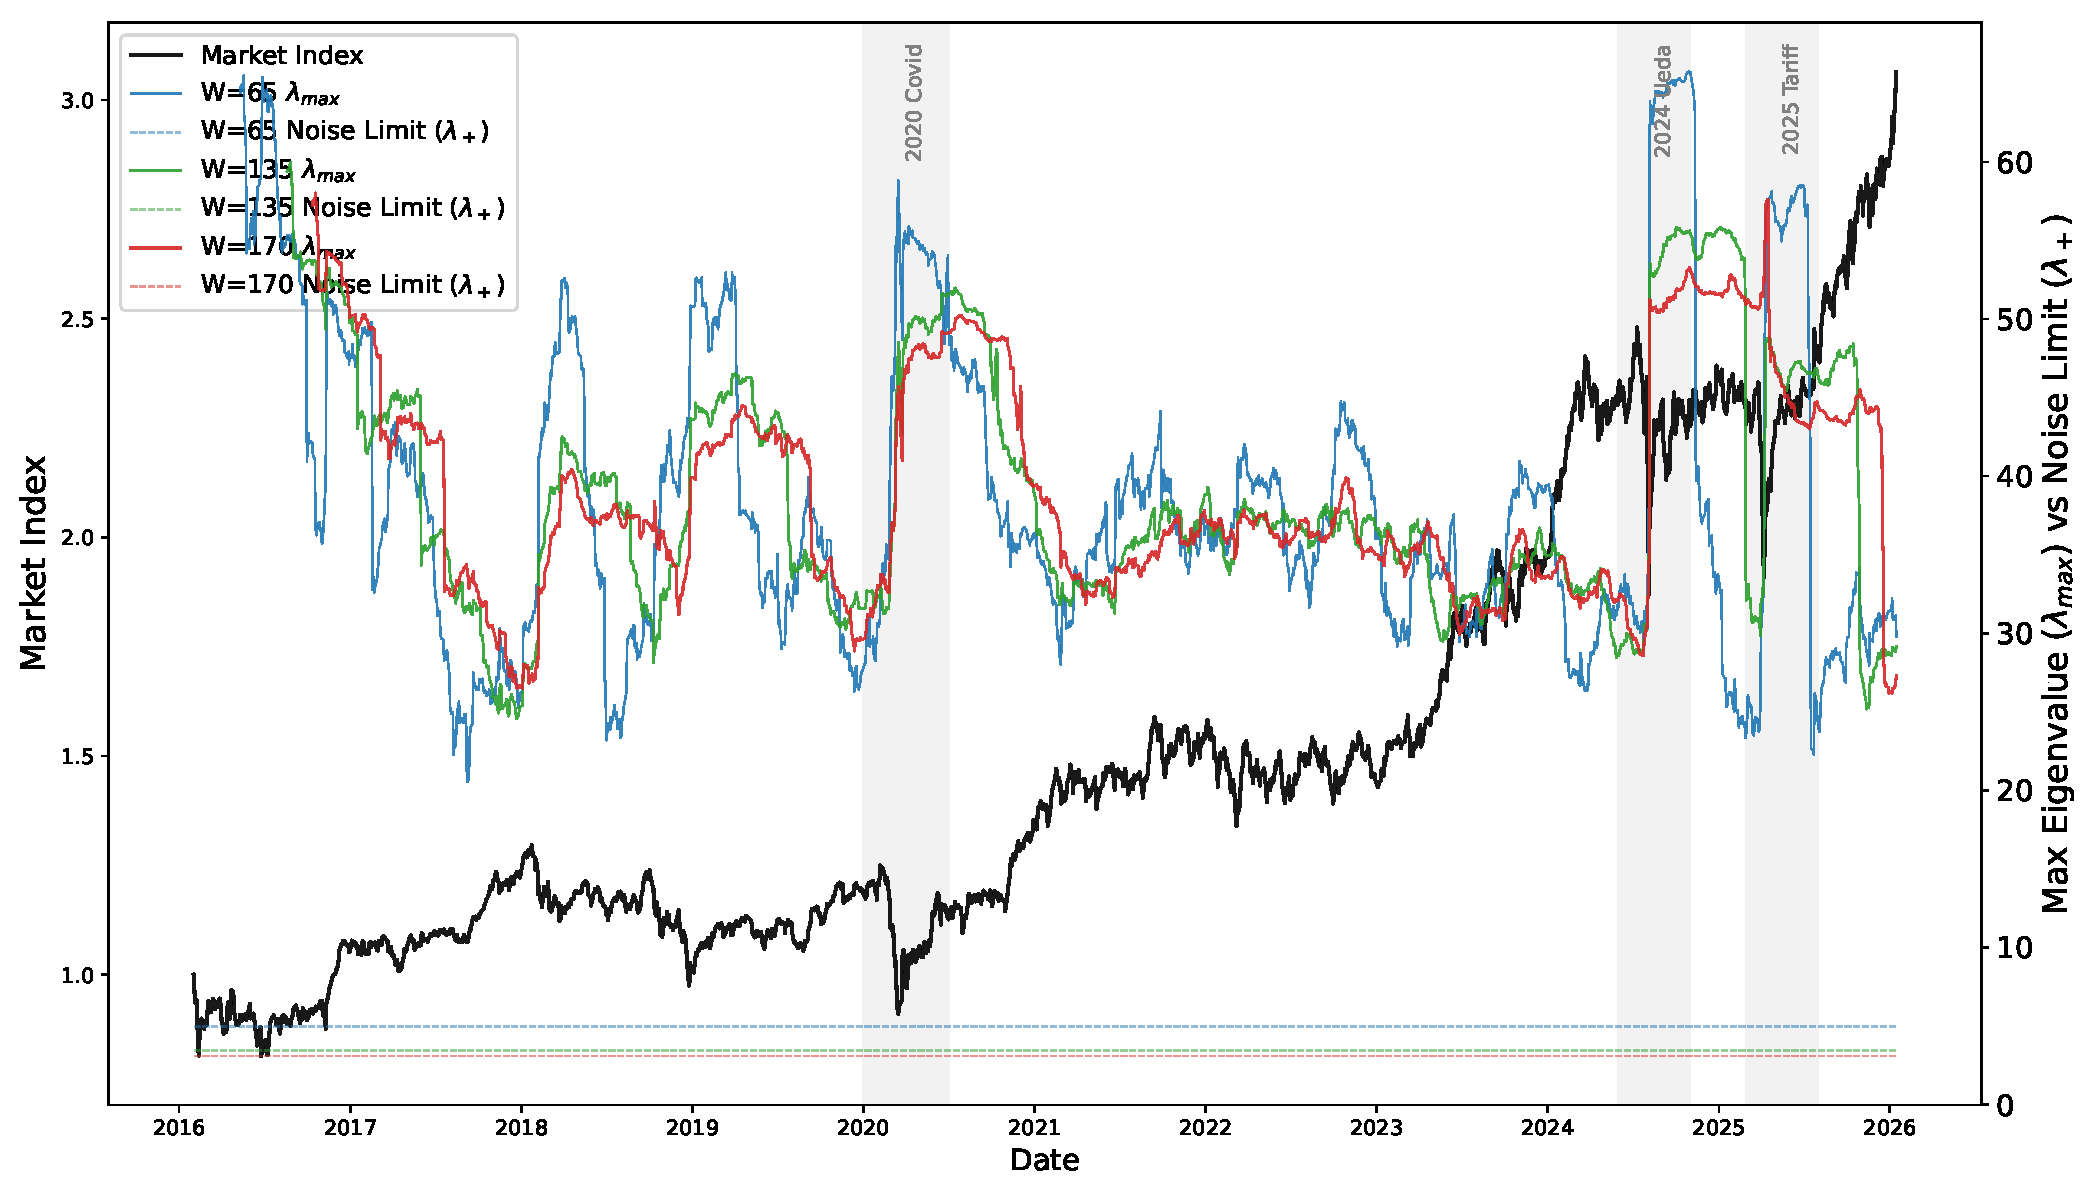
\includegraphics[width=1.0\linewidth]{figures/fig_5_1.pdf} % 先ほどのRMTプロット画像
  \caption{市場指数とRMT最大固有値($\lambda_{max}$)の時系列推移。点線はマルチェンコ・パスツール分布から導出される理論的ノイズ限界($\lambda_{+}$)を表す。}
  \label{fig:rmt_signal}
\end{figure}

同図より、全期間を通じて $\lambda_{max}$ は理論的ノイズ限界 $\lambda_{+}$ を大きく上回って推移していることが確認できる（$\lambda_{max} \gg \lambda_{+}$）。
従来のRMT研究において、$\lambda_{+}$ 以下の固有値はノイズとして除去されるが、本結果は、TOPIX100市場においては平常時であっても極めて強い「マーケット・モード（市場全体の同期）」が存在し、系が常に秩序化された準安定状態にあることを示唆している。
したがって、本研究ではノイズ除去処理を行わず、$\lambda_{max}$ の絶対値およびその変動を直接的な「同期圧力の指標」として監視することが物理的に妥当であると結論付けた。

\subsubsection{評価指標と検証用データセット}
次に、最適な窓幅 $W$ を定量的に決定するため、暴落予測において最も重視される「再現率（Recall）」を用いた感度分析を行う。
暴落予測において最も回避すべき事象は、致命的な下落を見逃すこと（False Negative）である。しかし、すべての暴落が同等の被害をもたらすわけではない。例えば、通常の軽い下落（-3\%程度）の見逃しと、金融危機（-10\%超）の見逃しを等価に扱うことは、実務的なリスク管理の観点から不適切である。

そこで本研究では、以下の2種類の再現率（Recall）を定義し、モデルの性能を多角的に評価する。
\begin{enumerate}
    \item \textbf{通常リコール (Normal Recall):}
    発生した暴落イベントの「日数（頻度）」に対し、モデルが正しくアラートを発した割合。物理的には「イベントの発生確率」に対する検知能力を示す。
    \begin{equation}
      Recall_{norm} = \frac{\sum_{t \in E_{crash}} \mathbb{I}(\hat{y}_t = 1)}{|E_{crash}|}
    \end{equation}

    \item \textbf{重み付けリコール (Weighted Recall):}
    各暴落イベントにおける「市場インパクト（損失規模）」を重み $w_t$ とし、全期間の総損失に対し、モデルが検知によって回避可能であった損失の割合。物理的には「解放された総ポテンシャルエネルギー」に対する検知能力を示す。
    \begin{equation}
    w(t) = w_{base} \times \underbrace{\exp(-\gamma \cdot \Delta t)}_{\text{時間減衰項}} \times \underbrace{\frac{|R(t)|}{|\theta|}}_{\text{強度比例項}}
    \end{equation}
\end{enumerate}

本実験では、以下の性質の異なる3つの期間を用いてウォークフォワード検証を行い、その平均Recallを評価指標とした。

\begin{itemize}
    \item \textbf{Scenario 1: 2020 Covid (2020/01 -- 2020/06):} 未知の感染症によるパニック的な暴落。
    \item \textbf{Scenario 2: 2024 Ueda (2024/06 -- 2024/10):} 金融政策変更（利上げ）に起因する急激な調整。
    \item \textbf{Scenario 3: 2025 Tariff (2025/03 -- 2025/07):} 関税政策と地政学リスクによる暴落。
\end{itemize}

\subsubsection{結果と考察: 窓幅とターゲットの適合性}
図\ref{fig:5.2}および図\ref{fig:5.3}に、それぞれターゲット変数として「Index 1（時価総額加重指数）」と「Index 2（市場インパクト指数）」を用いた場合の窓幅感度を示す。
各図において、(a)は発生件数ベースの「通常Recall」、(b)は下落規模を考慮した「重み付けRecall」の結果である。

\begin{figure}[H]
\centering

\begin{subfigure}{1.0\textwidth}
\centering
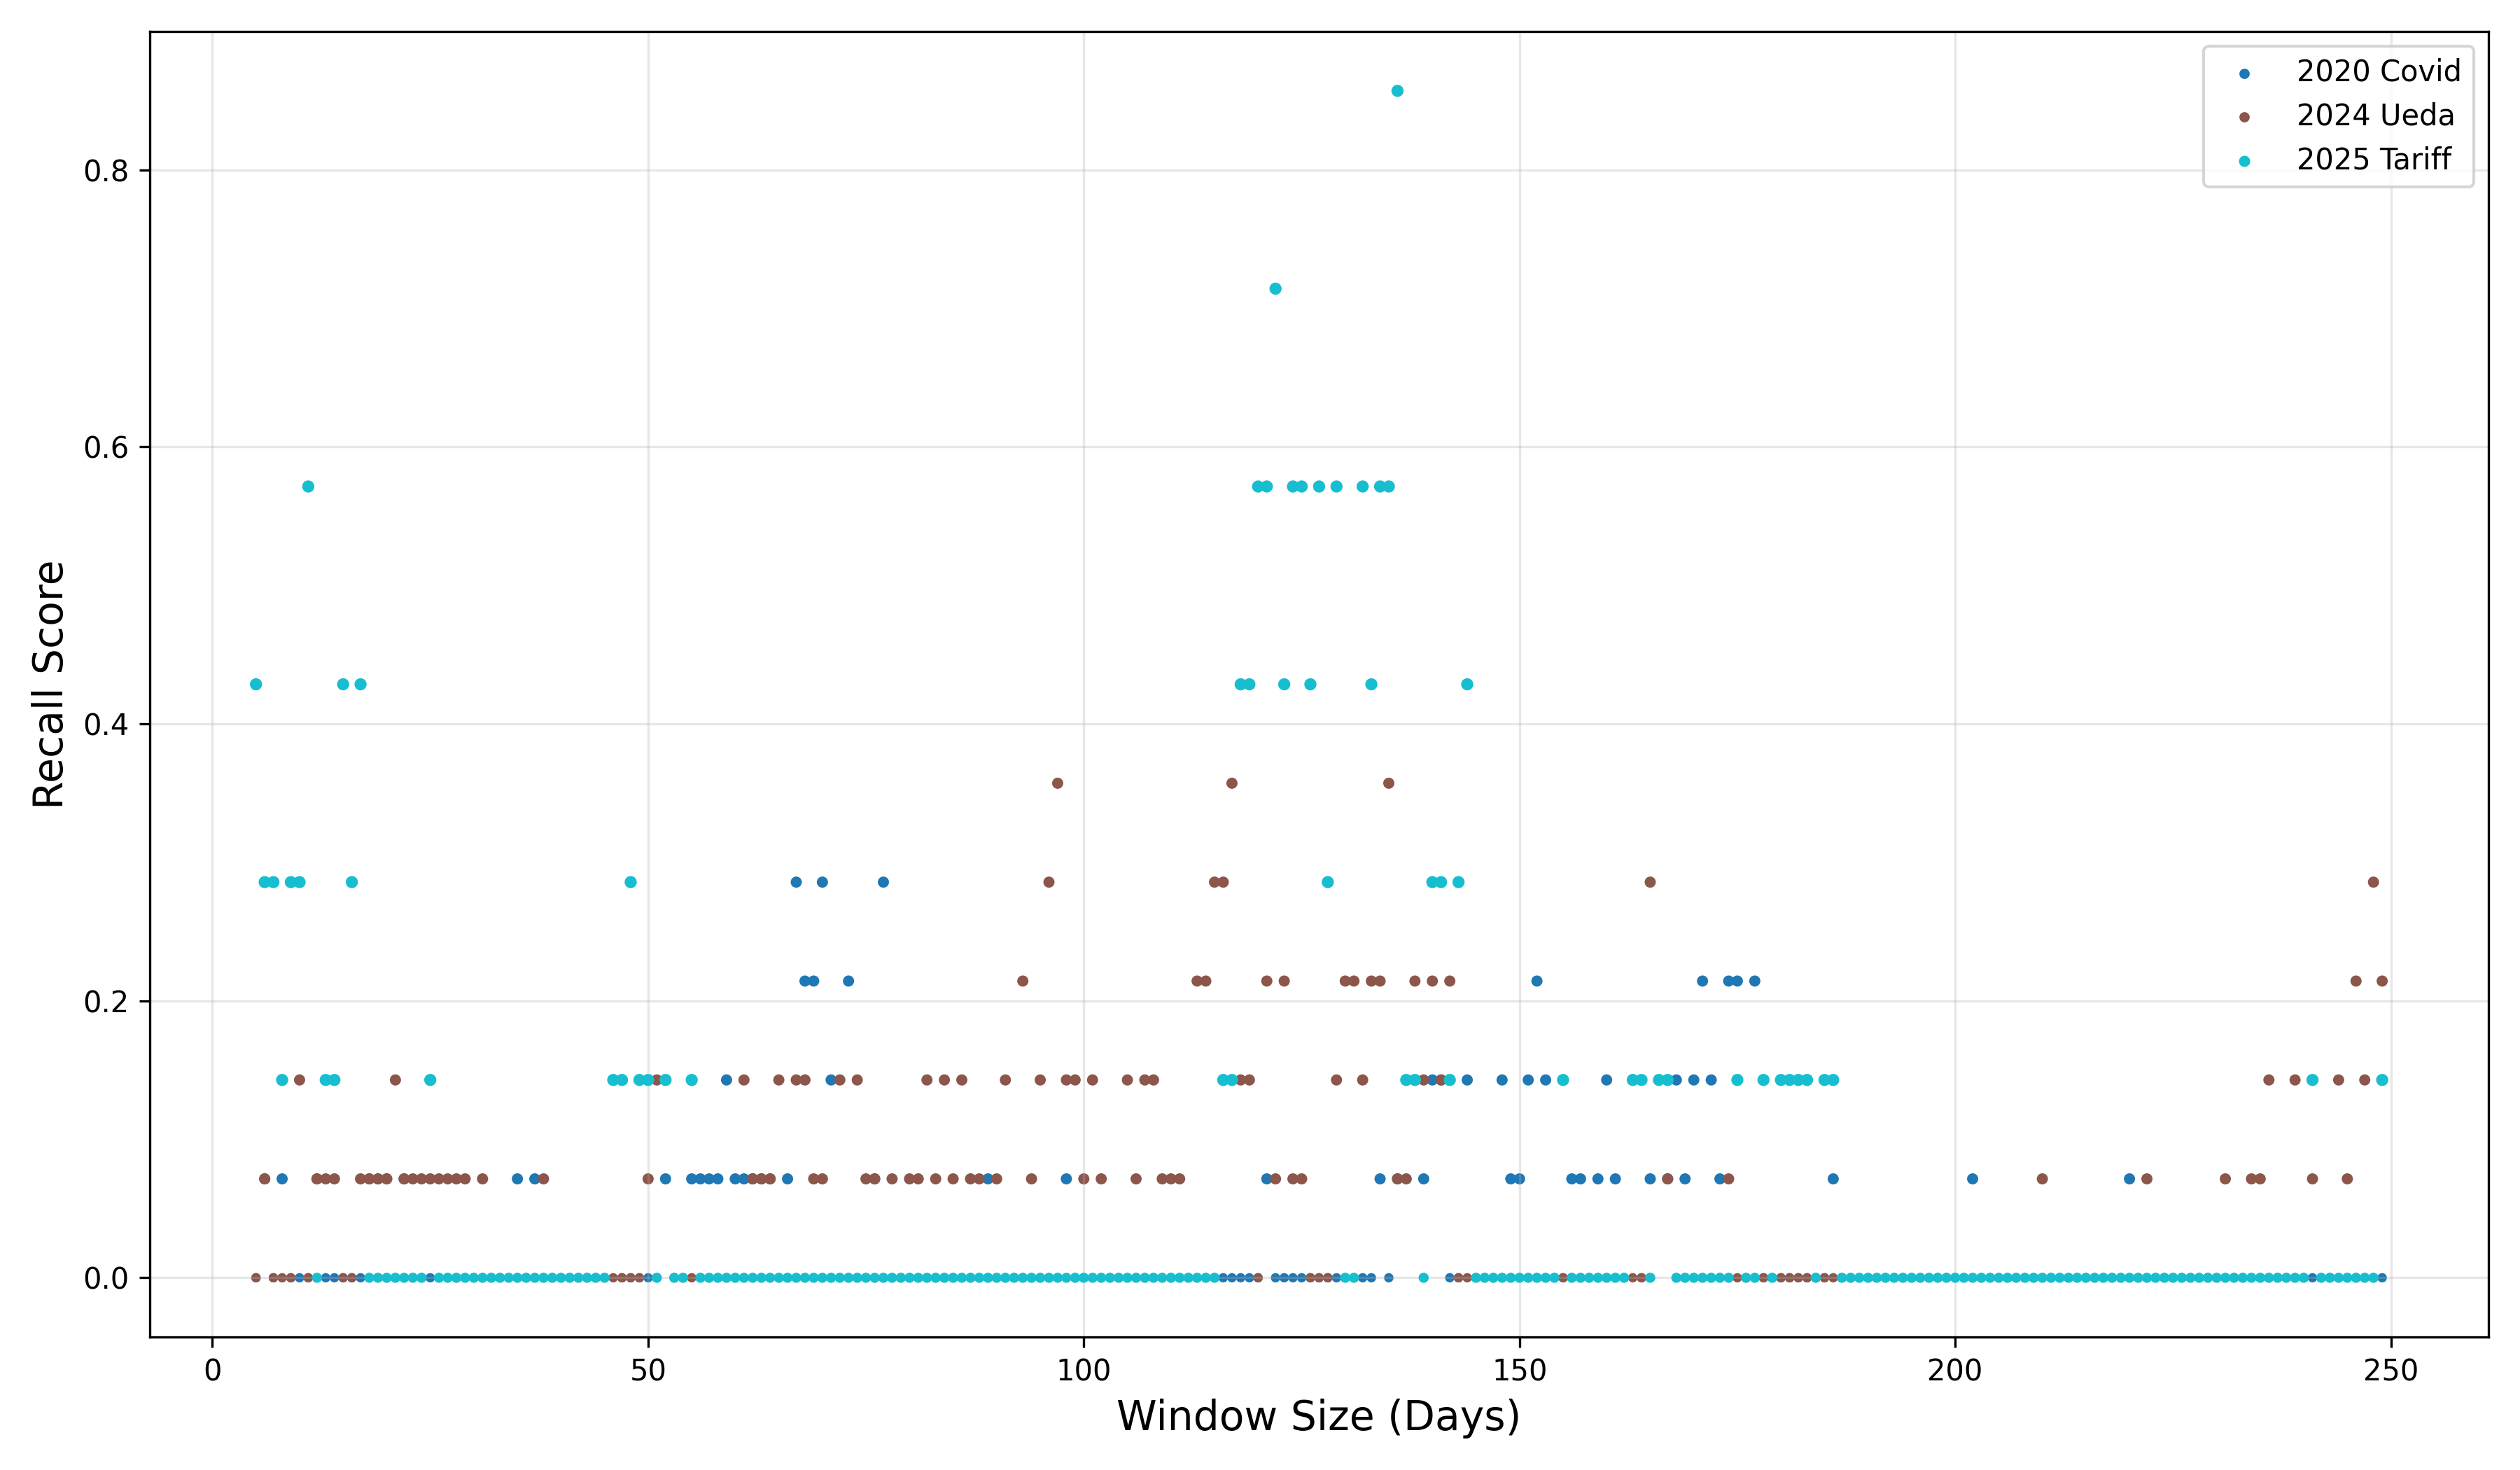
\includegraphics[width=\textwidth]{figures/fig_5_2a.png}
\caption{リコールスコアの窓幅依存性}
\label{fig:5.2a}
\end{subfigure}
\hfill
\begin{subfigure}{1.0\textwidth}
\centering
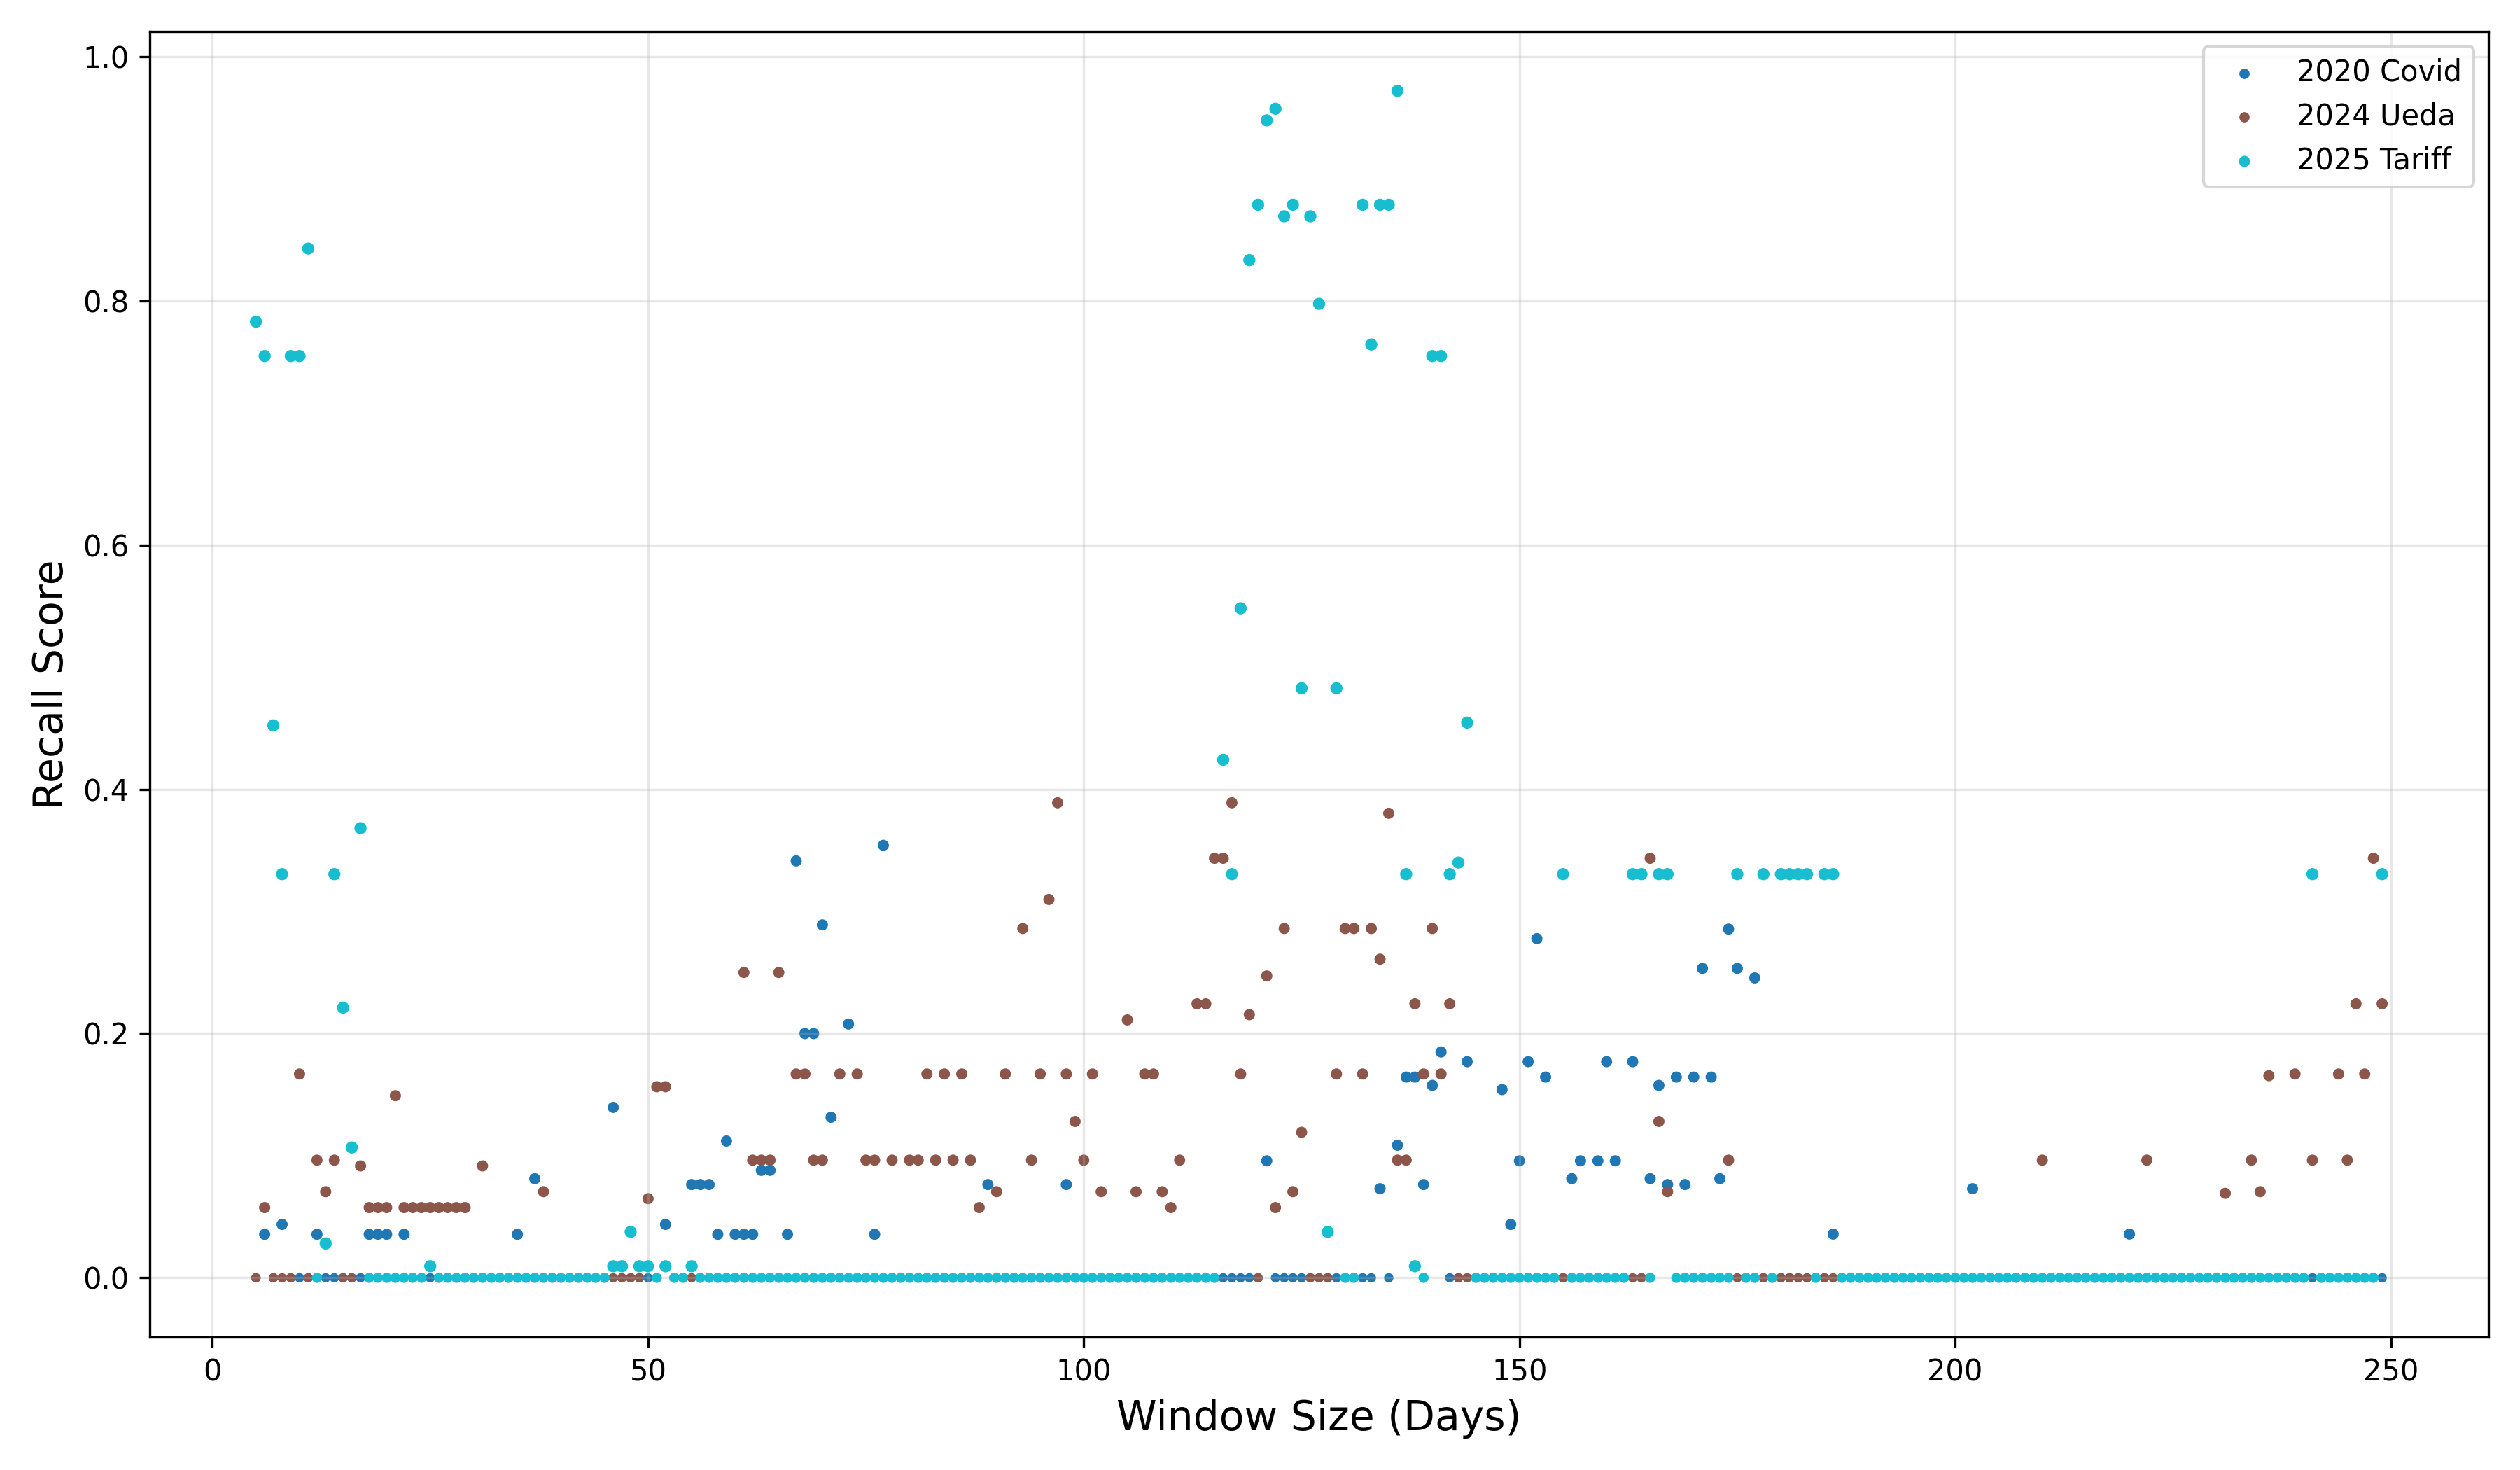
\includegraphics[width=\textwidth]{figures/fig_5_2b.png}
\caption{リコールスコア（重みづけ）の窓幅依存性}
\label{fig:5.2b}
\end{subfigure}
\caption{リコールスコアの窓幅依存性（インデックス1）}
\label{fig:5.2}
\end{figure}

\begin{figure}[H]
\centering
\begin{subfigure}{1.0\textwidth}
\centering
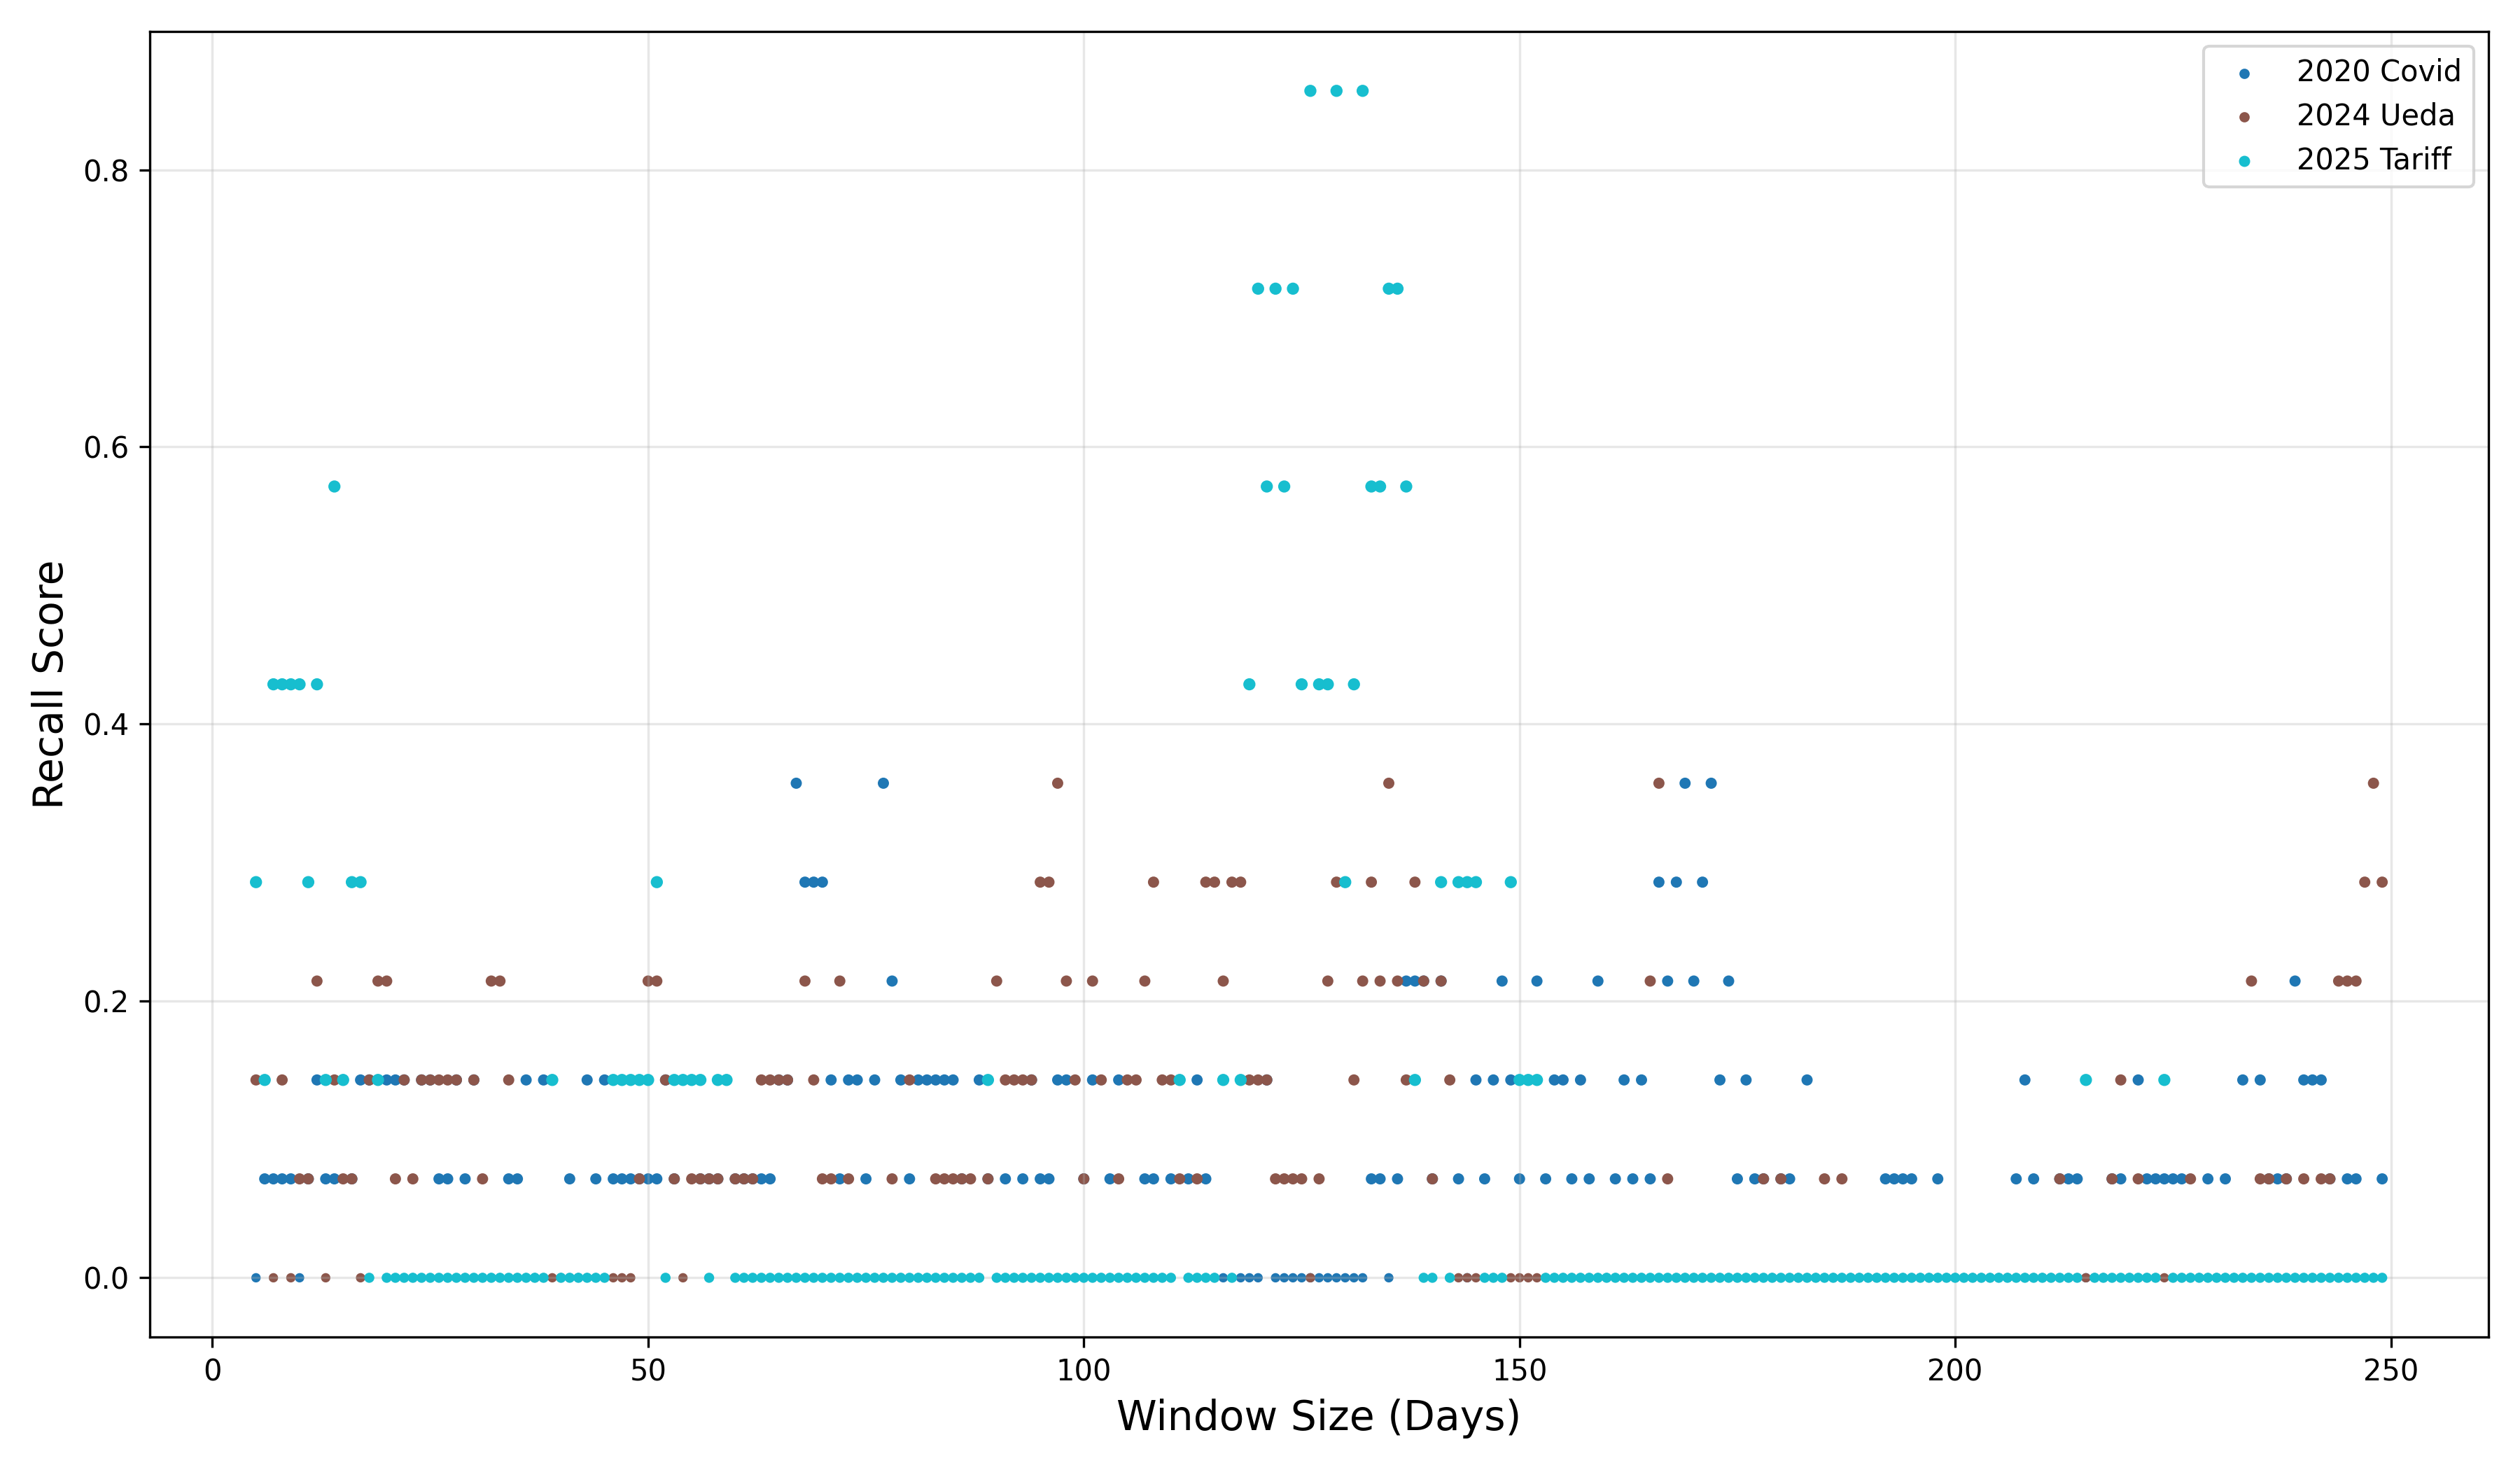
\includegraphics[width=\textwidth]{figures/fig_5_3a.png}
\caption{リコールスコアの窓幅依存性}
\label{fig:5.3a}
\end{subfigure}
\hfill
\begin{subfigure}{1.0\textwidth}
\centering
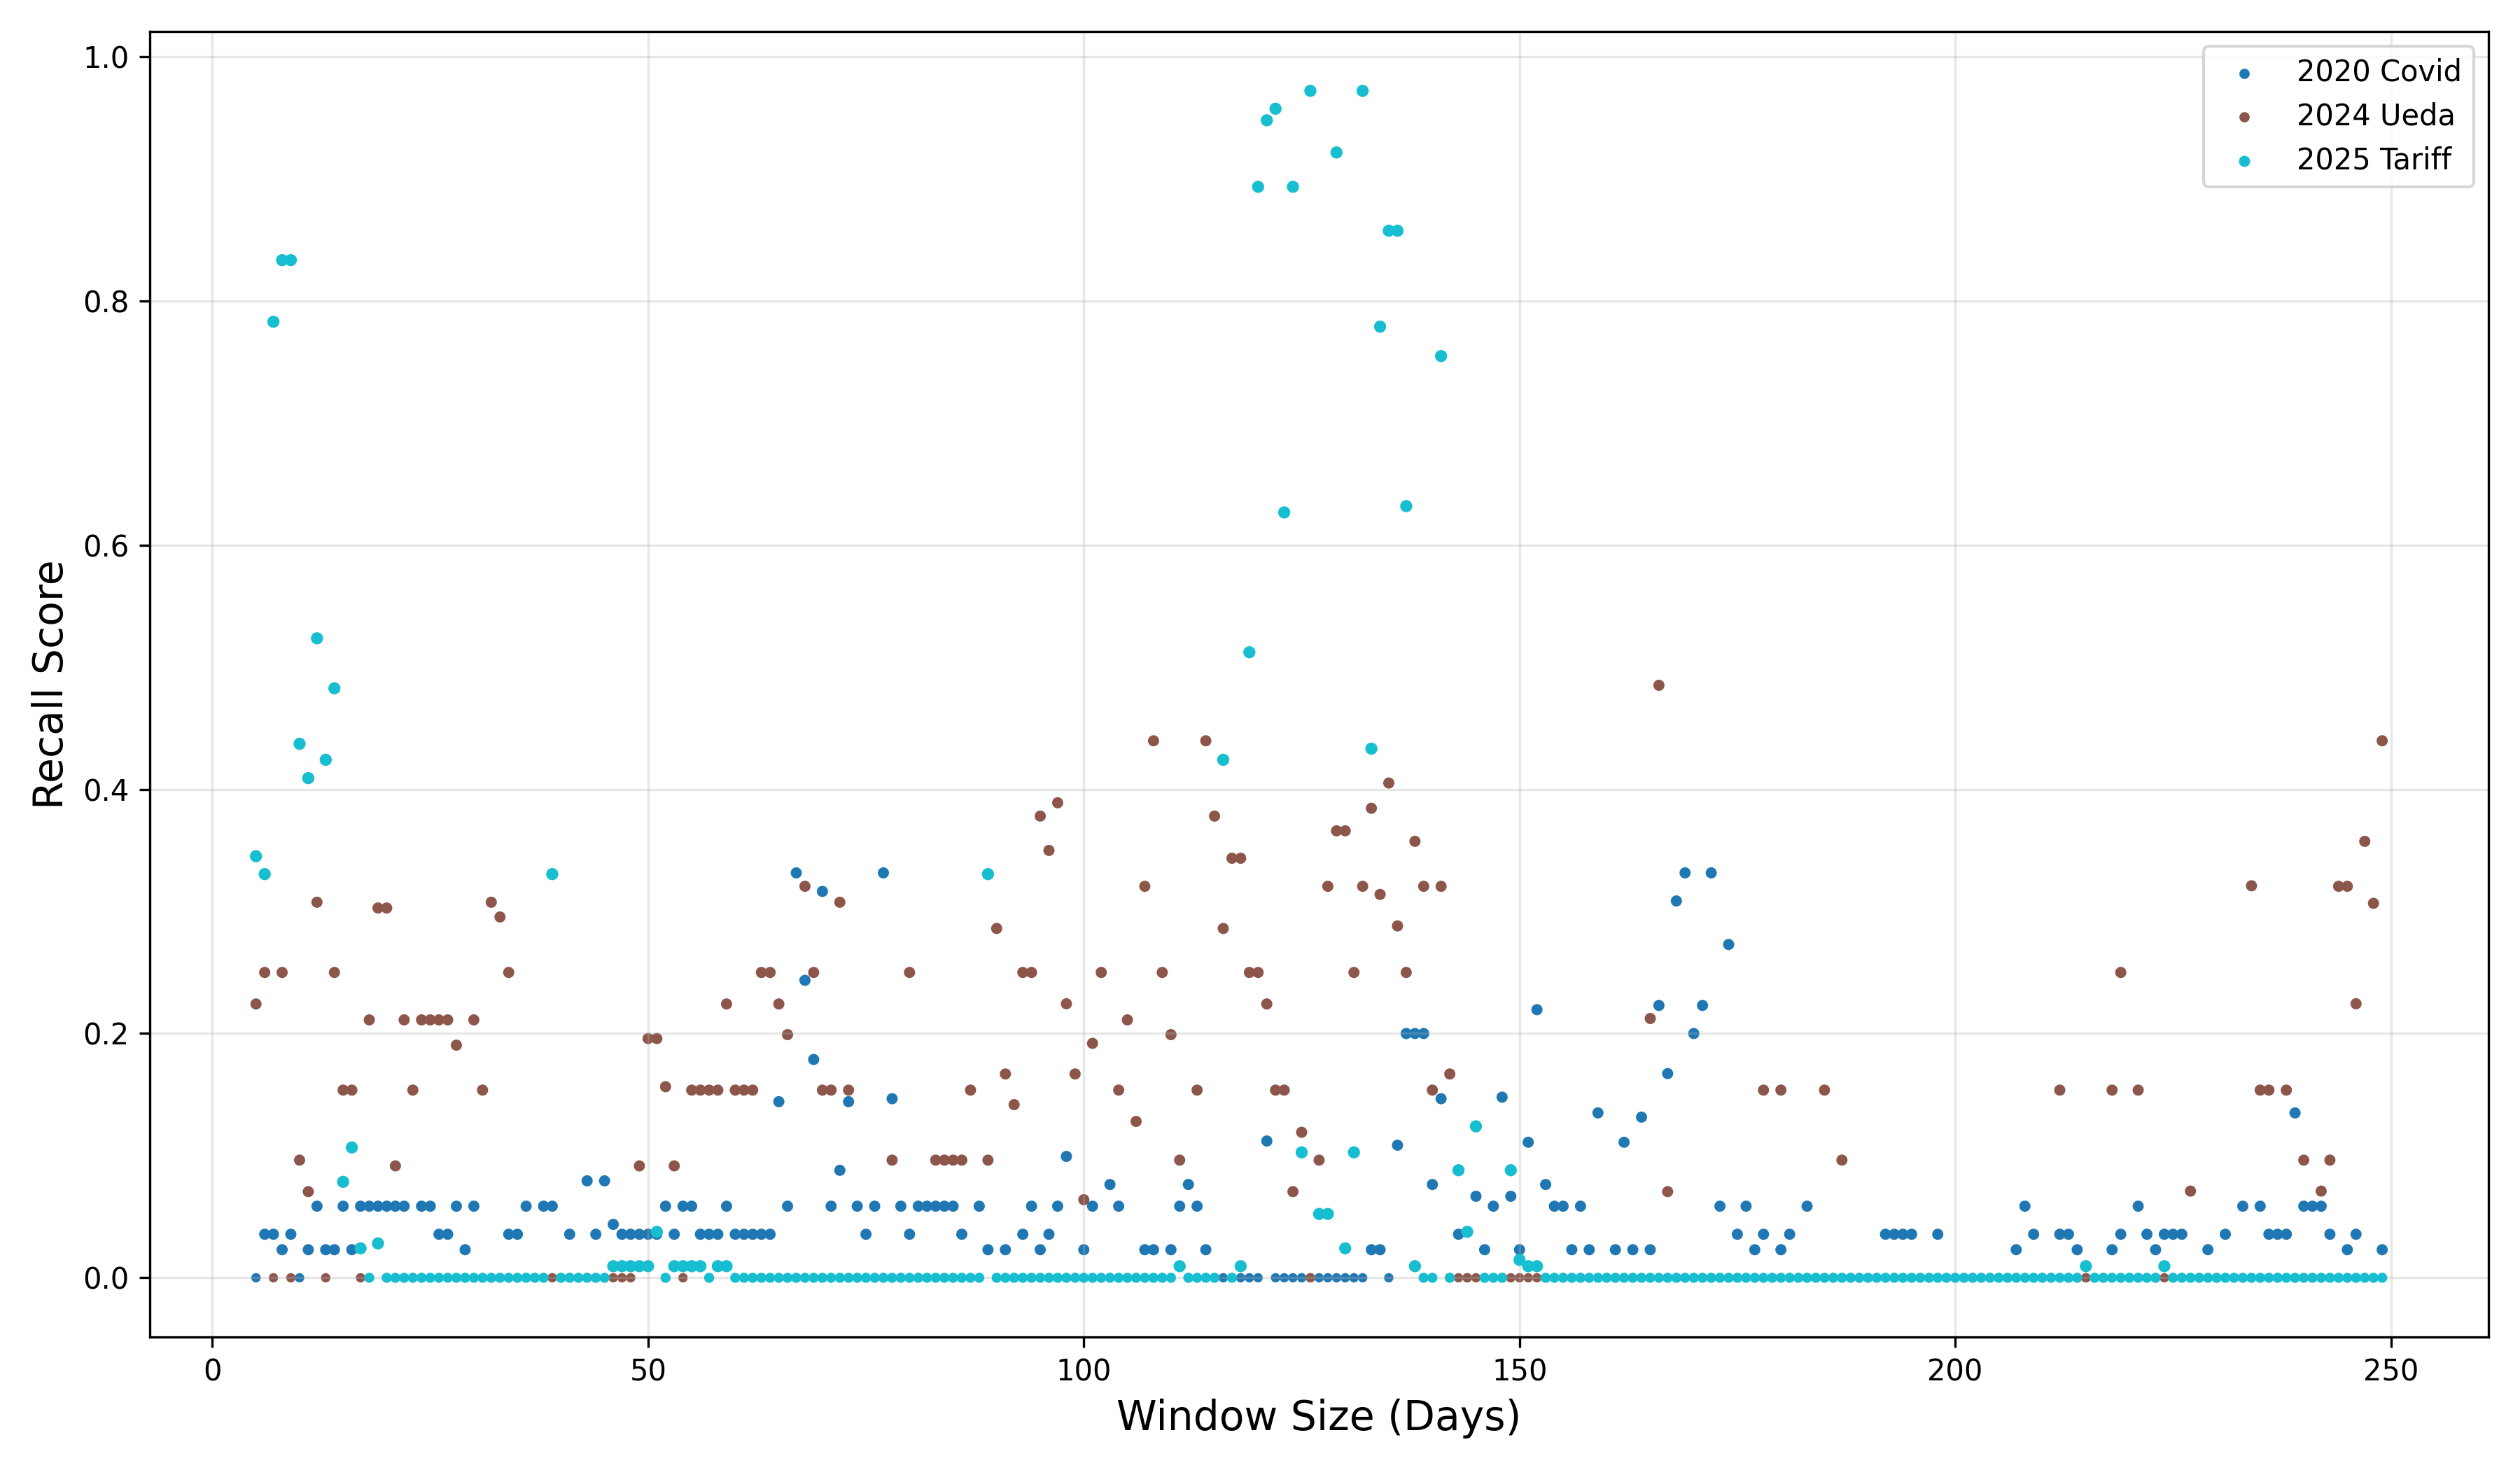
\includegraphics[width=\textwidth]{figures/fig_5_3b.png}
\caption{リコールスコア（重みづけ）の窓幅依存性}
\label{fig:5.3b}
\end{subfigure}
\caption{リコールスコアの窓幅依存性（インデックス2）}
\label{fig:5.3}
\end{figure}

\clearpage
これらの結果を比較・分析したところ、以下の重要な知見が得られた。

\begin{enumerate}
    \item \textbf{Index 2 における「見逃し」の抑制:}
    図\ref{fig:5.3}（Index 1）と図\ref{fig:5.3}（Index 2）を比較すると、平均的なRecallの水準そのものには劇的な差異は見られない。しかし、詳細に見ると、Index 1 では特定のリスクシナリオにおいてRecallが完全に0となる（致命的な見逃しが発生する）ケースが散見されるのに対し、Index 2 では同条件下でも僅かながら数値を維持し、完全な見逃しを回避する傾向が確認された。これは、Index 2 が物理的なエネルギー解放（大規模な下落）を重み付けして学習するため、ノイズに埋もれがちな微弱なシグナルに対しても、最低限の応答性能を維持しているためと推察される。

    \item \textbf{シナリオ依存性と共通のクリティカルレンジ:}
    両インデックスにおいて、Recallが高くなる（ピークとなる）窓幅の範囲は概ね一致している。これは、最適な窓幅がターゲットの定義（Index 1か2か）よりも、各シナリオにおける暴落の物理的性質（タイムスケールや衝撃の伝播速度）に強く依存していることを示唆している。すなわち、シナリオごとに「クリティカルな窓枠範囲」が存在し、それはインデックスの定義に関わらず共通して観測される現象である。

    \item \textbf{長期窓 ($W=135$) の選定理由:}
    両図において、$W=135$ 近辺は比較的安定した感度を示している。この領域は、前述の通り $Q = W/N > 1$ を満たす数学的に安定な領域である。現段階では Index 2 が圧倒的に優れているとは断定できないものの、Index 1 で見られるような不安定な挙動（ゼロへの急落）が抑制されている点を評価し、本研究では Index 2 を採用する。
\end{enumerate}

以上の一次スクリーニングの結果、本研究ではRMTの窓幅として \textbf{$W=135$} を固定パラメータとして採用する。
次節以降においては、この $W=135$ を用いたモデルに対し、PR曲線による適合率とのトレードオフや、経済的リターンへの寄与を含めた多角的な視点から、Index 2 の真価を詳細に検証する。

\subsection{予測精度の定量的評価とモデル解釈}
本節では、提案モデルの予測性能を定量的に評価すると同時に、SHAP分析および時系列のミクロ挙動解析を用いて、モデルが物理的に何を根拠に暴落を予知しているのかを解明する。
評価は、短期的な「Scenario 1（トランプ関税ショック期）」と、長期的な「Scenario 2（植田～トランプ期）」の2つの期間において、ターゲット変数（Index 1 vs Index 2）ごとの挙動を比較する形で行う。

\subsubsection{評価指標：PR曲線とAUC}
モデルの予測性能を評価する指標として、前節の再現率（Recall）に加え、適合率（Precision）を導入する。
\begin{equation}
  Precision = \frac{TP}{TP + FP} = \frac{\text{正しく予知できた暴落}}{\text{モデルが発した全アラート数}}
\end{equation}
再現率は「見逃しのなさ（センサー感度）」を、適合率は「信頼性」を表す。機械学習モデルは出力確率に対する「判定閾値（Threshold）」によってこれらをトレードオフの関係として調整する。この関係を可視化したものがPR曲線（Precision-Recall Curve）であり、曲線が右上（AUCが大きい）にあるほど高性能なモデルであることを示す。

\subsection{マクロ評価：シナリオ別予測精度}

\subsubsection{Scenario 1: トランプ関税ショック期における評価}
まず、本研究の検証期間における最後のイベントであり、モデルが十分な過去データを学習した状態で挑む「トランプ関税ショック期（2025/3/1 -- 2025/6/30）」の結果を分析する。

図\ref{fig:pr_scenario1}に、ターゲット変数ごとのPR曲線を示す。(a)はIndex 1（経済指標）、(b)はIndex 2（インパクト指標）の結果である。

\begin{figure}[H]
  \centering
  % --- 上段: Index 1 ---
  \begin{minipage}[b]{0.48\linewidth}
    \centering
    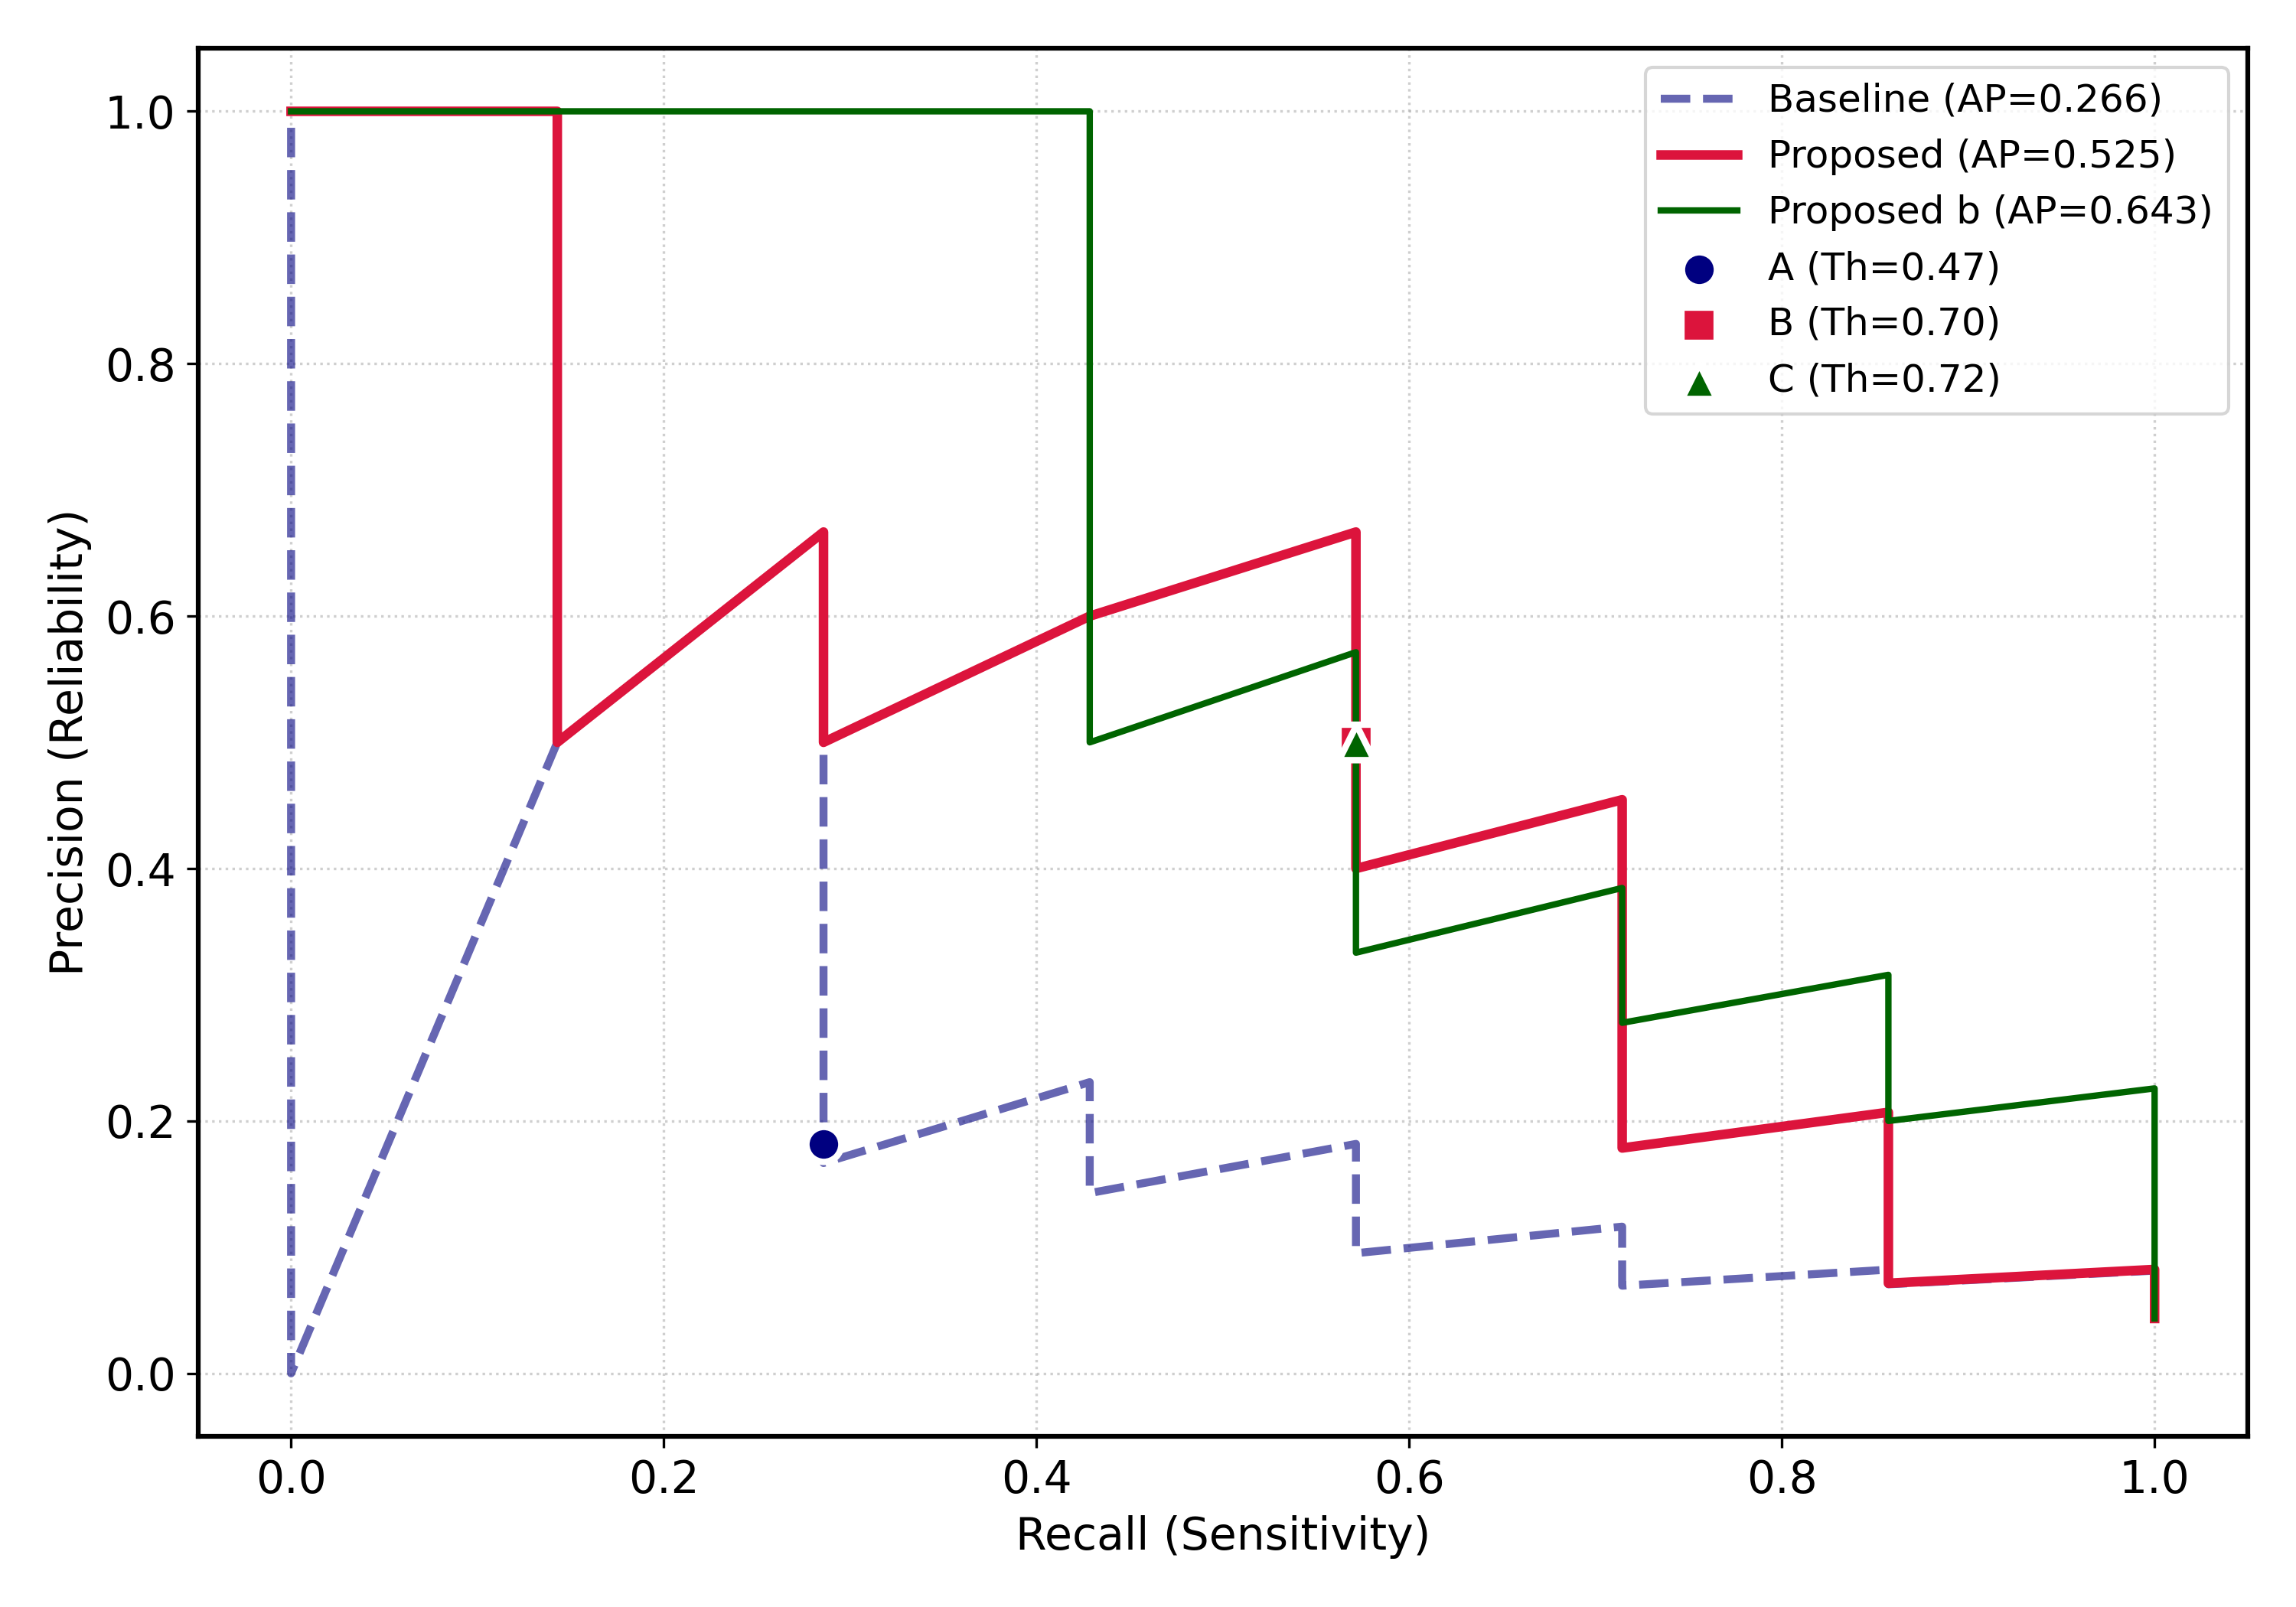
\includegraphics[width=\linewidth]{figures/fig_5_4a_pr(normal)_index1_scenario1.png}
    \caption*{(a) Index 1 / Normal PR}
  \end{minipage}
  \begin{minipage}[b]{0.48\linewidth}
    \centering
    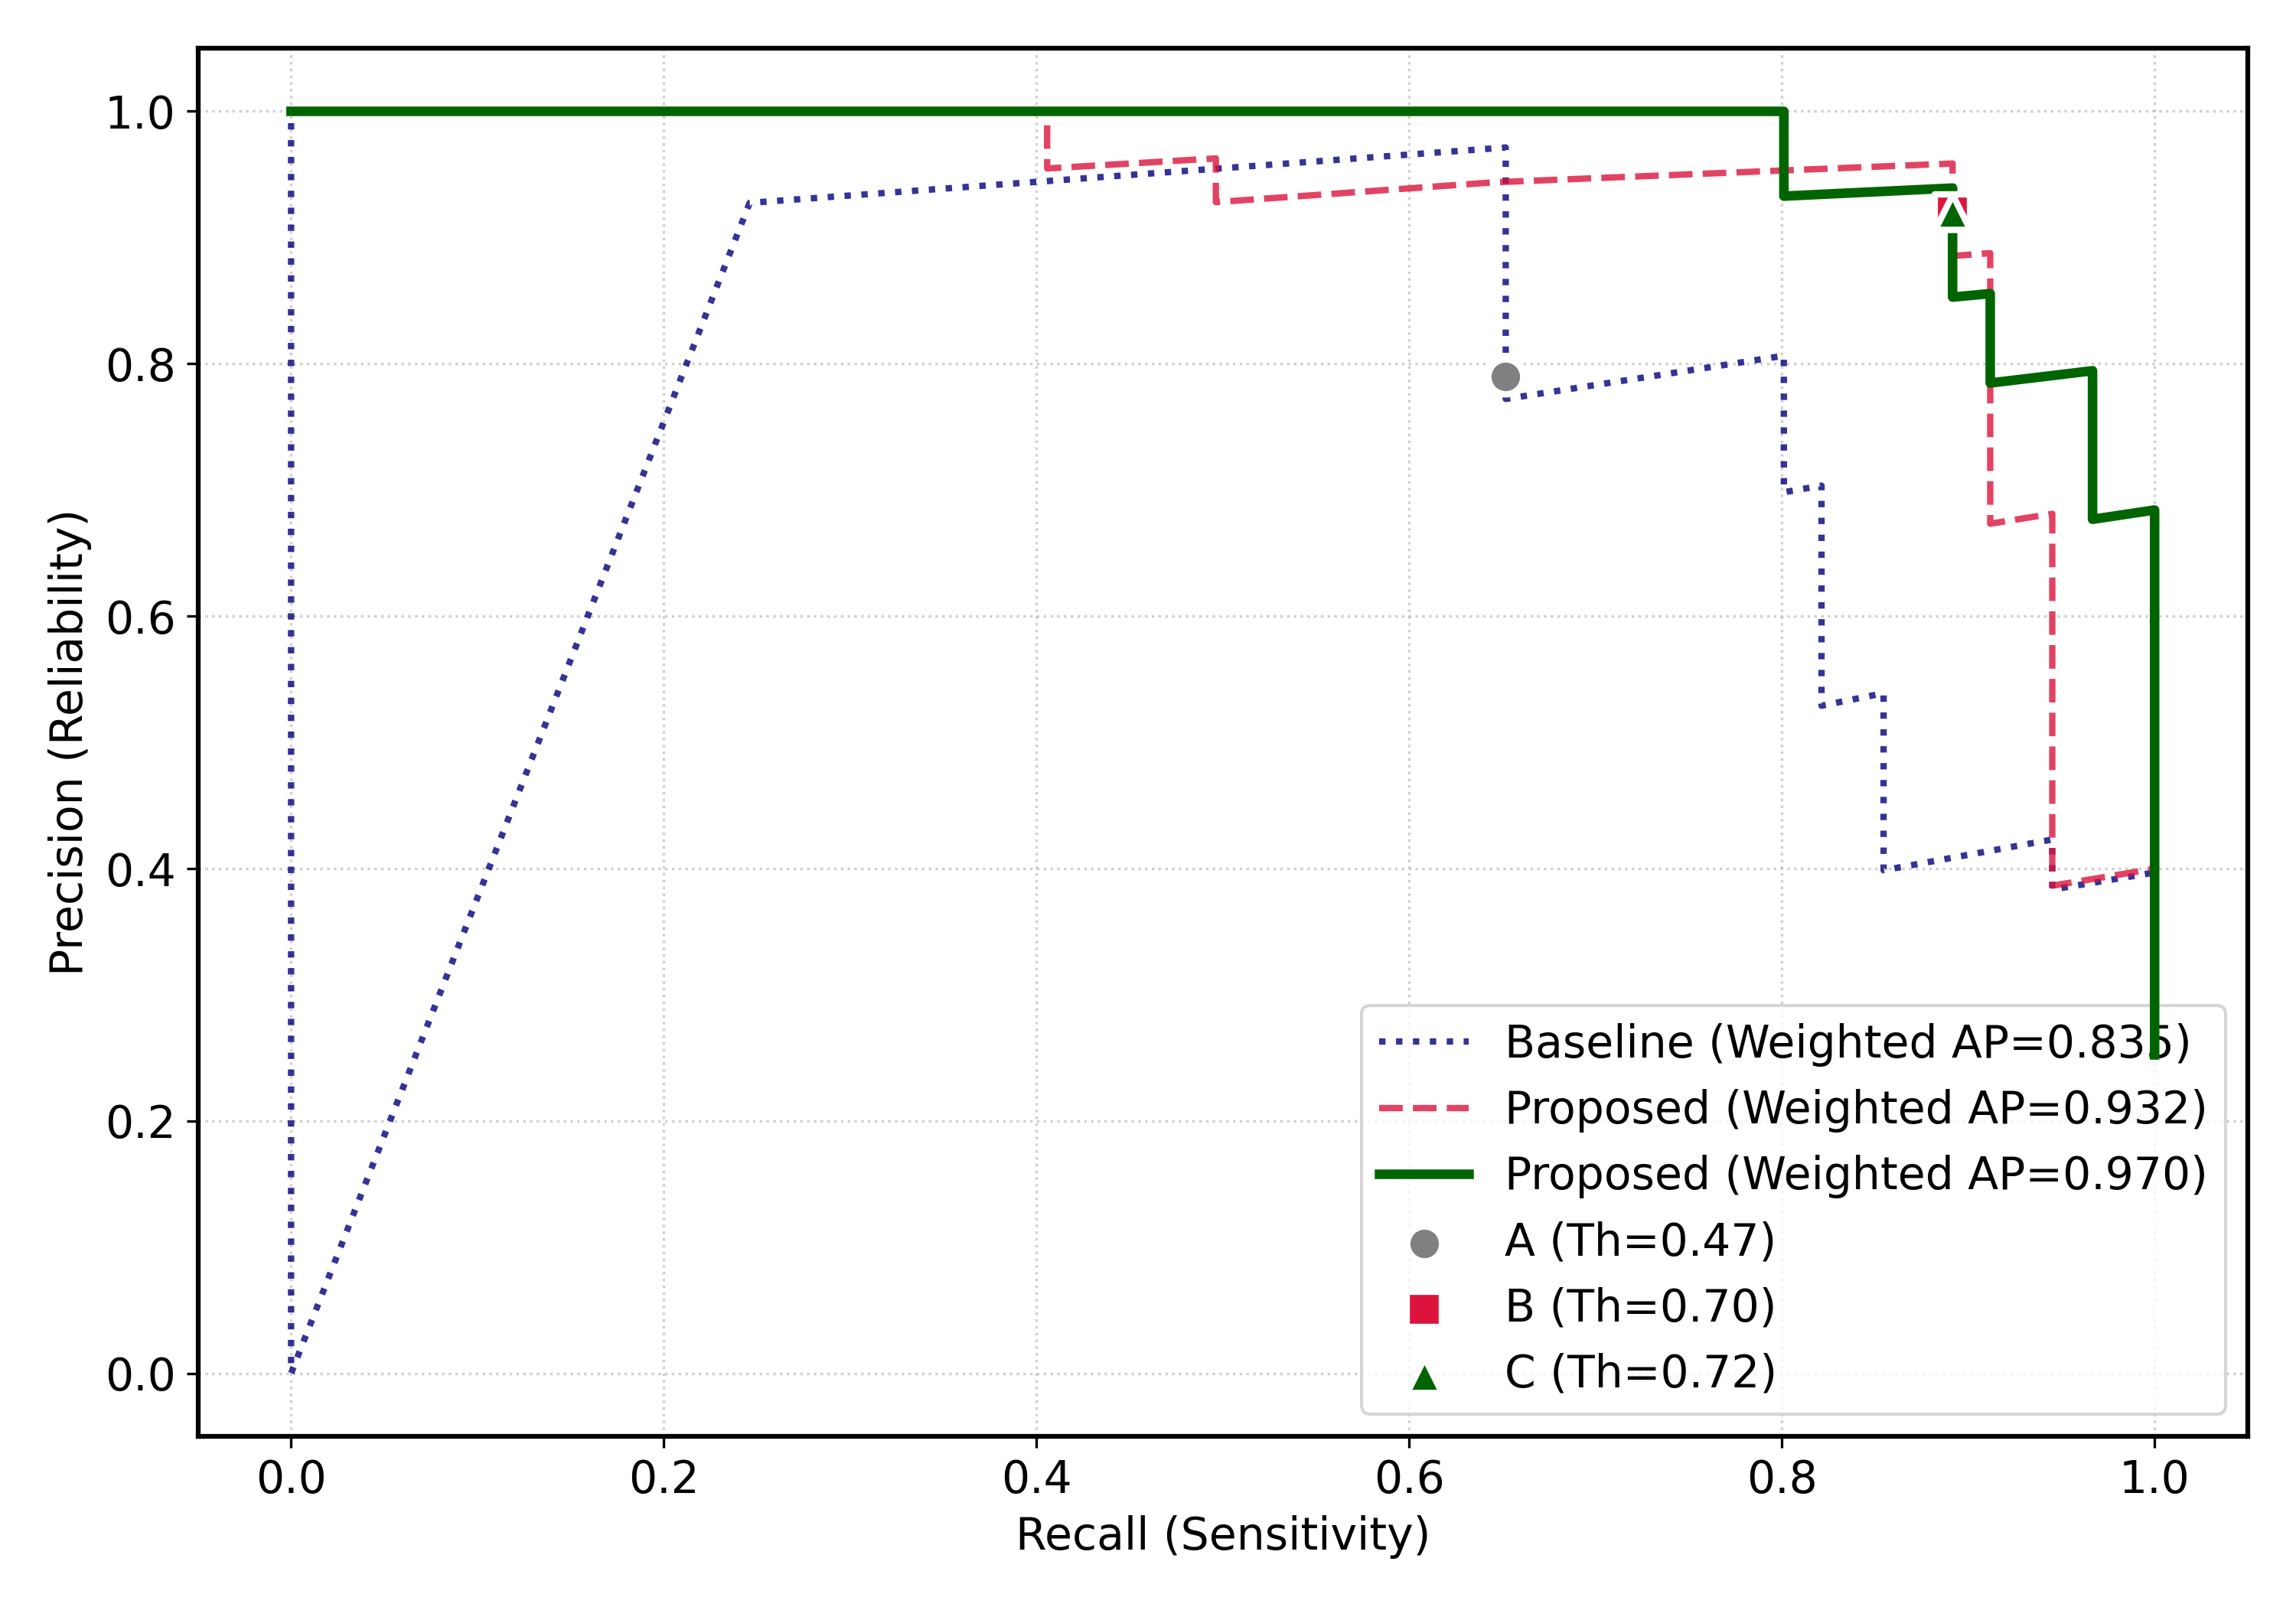
\includegraphics[width=\linewidth]{figures/fig_5_4b_pr(weight)_index1_scenario1.png}
    \caption*{(b) Index 1 / Weighted PR}
  \end{minipage}
  
  \vspace{0.5cm}
  
  % --- 下段: Index 2 ---
  \begin{minipage}[b]{0.48\linewidth}
    \centering
    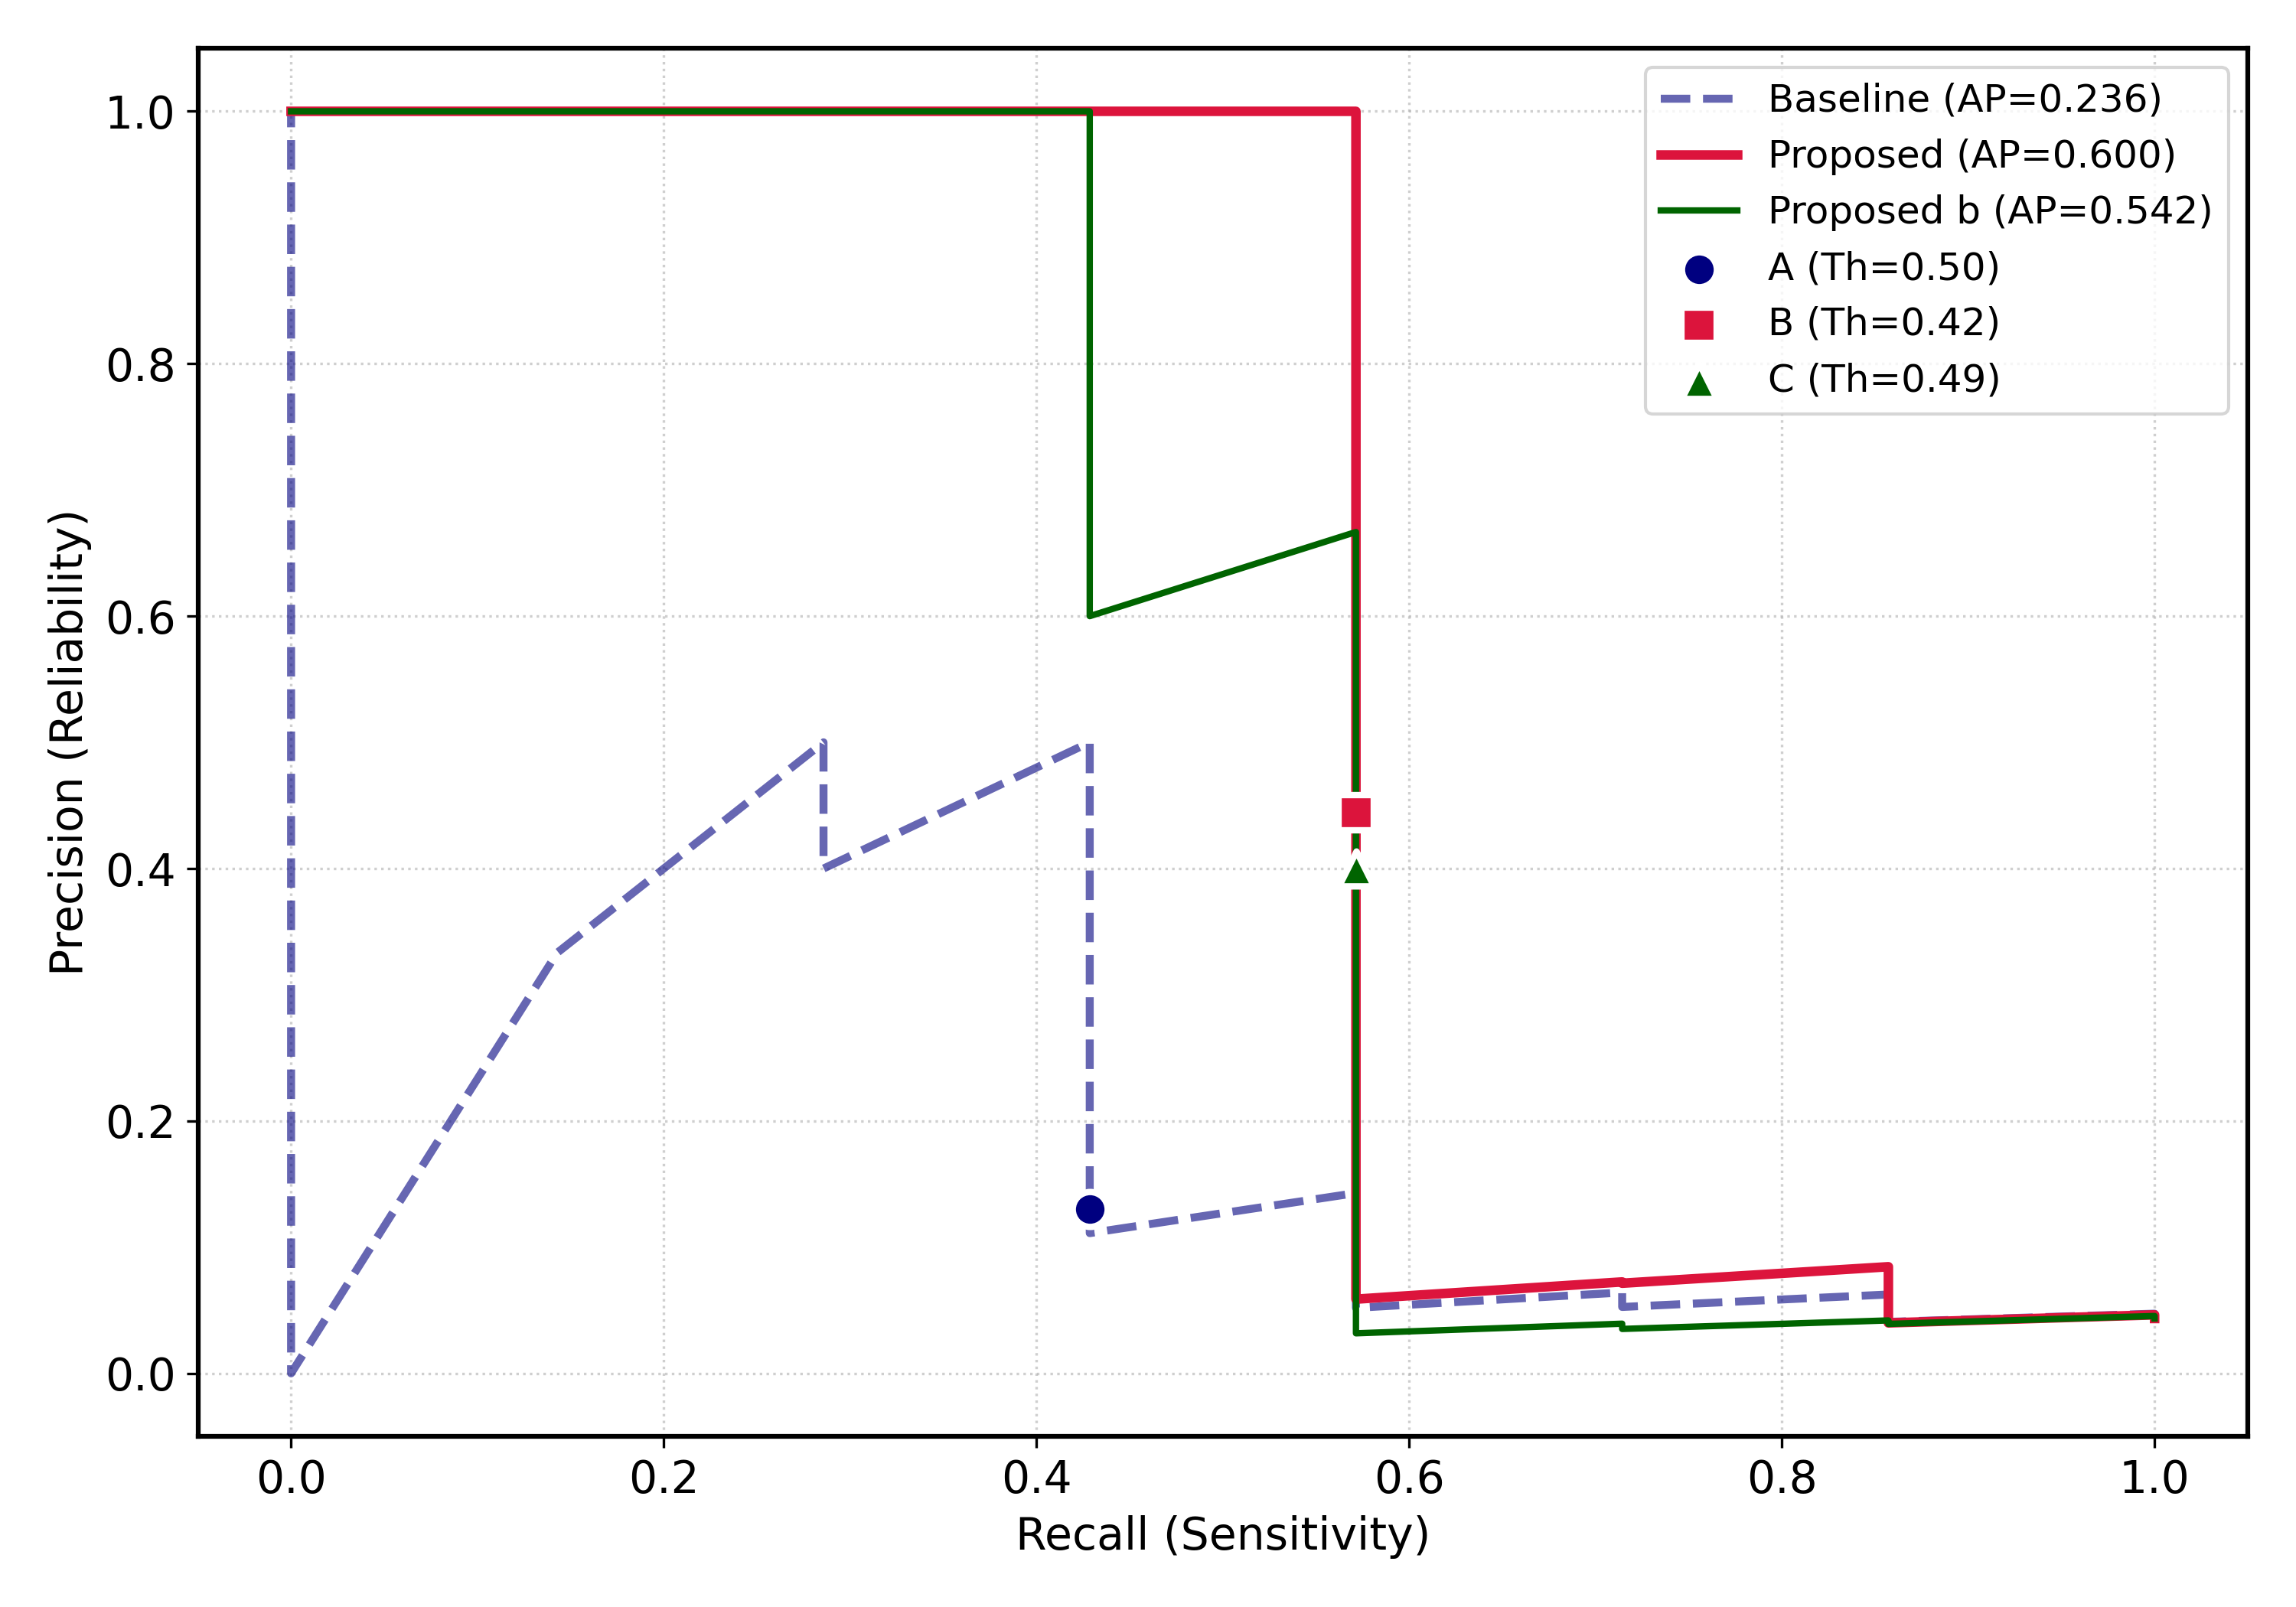
\includegraphics[width=\linewidth]{figures/fig_5_5a_pr(normal)_index2_scenario1.png}
    \caption*{(c) Index 2 / Normal PR}
  \end{minipage}
  \begin{minipage}[b]{0.48\linewidth}
    \centering
    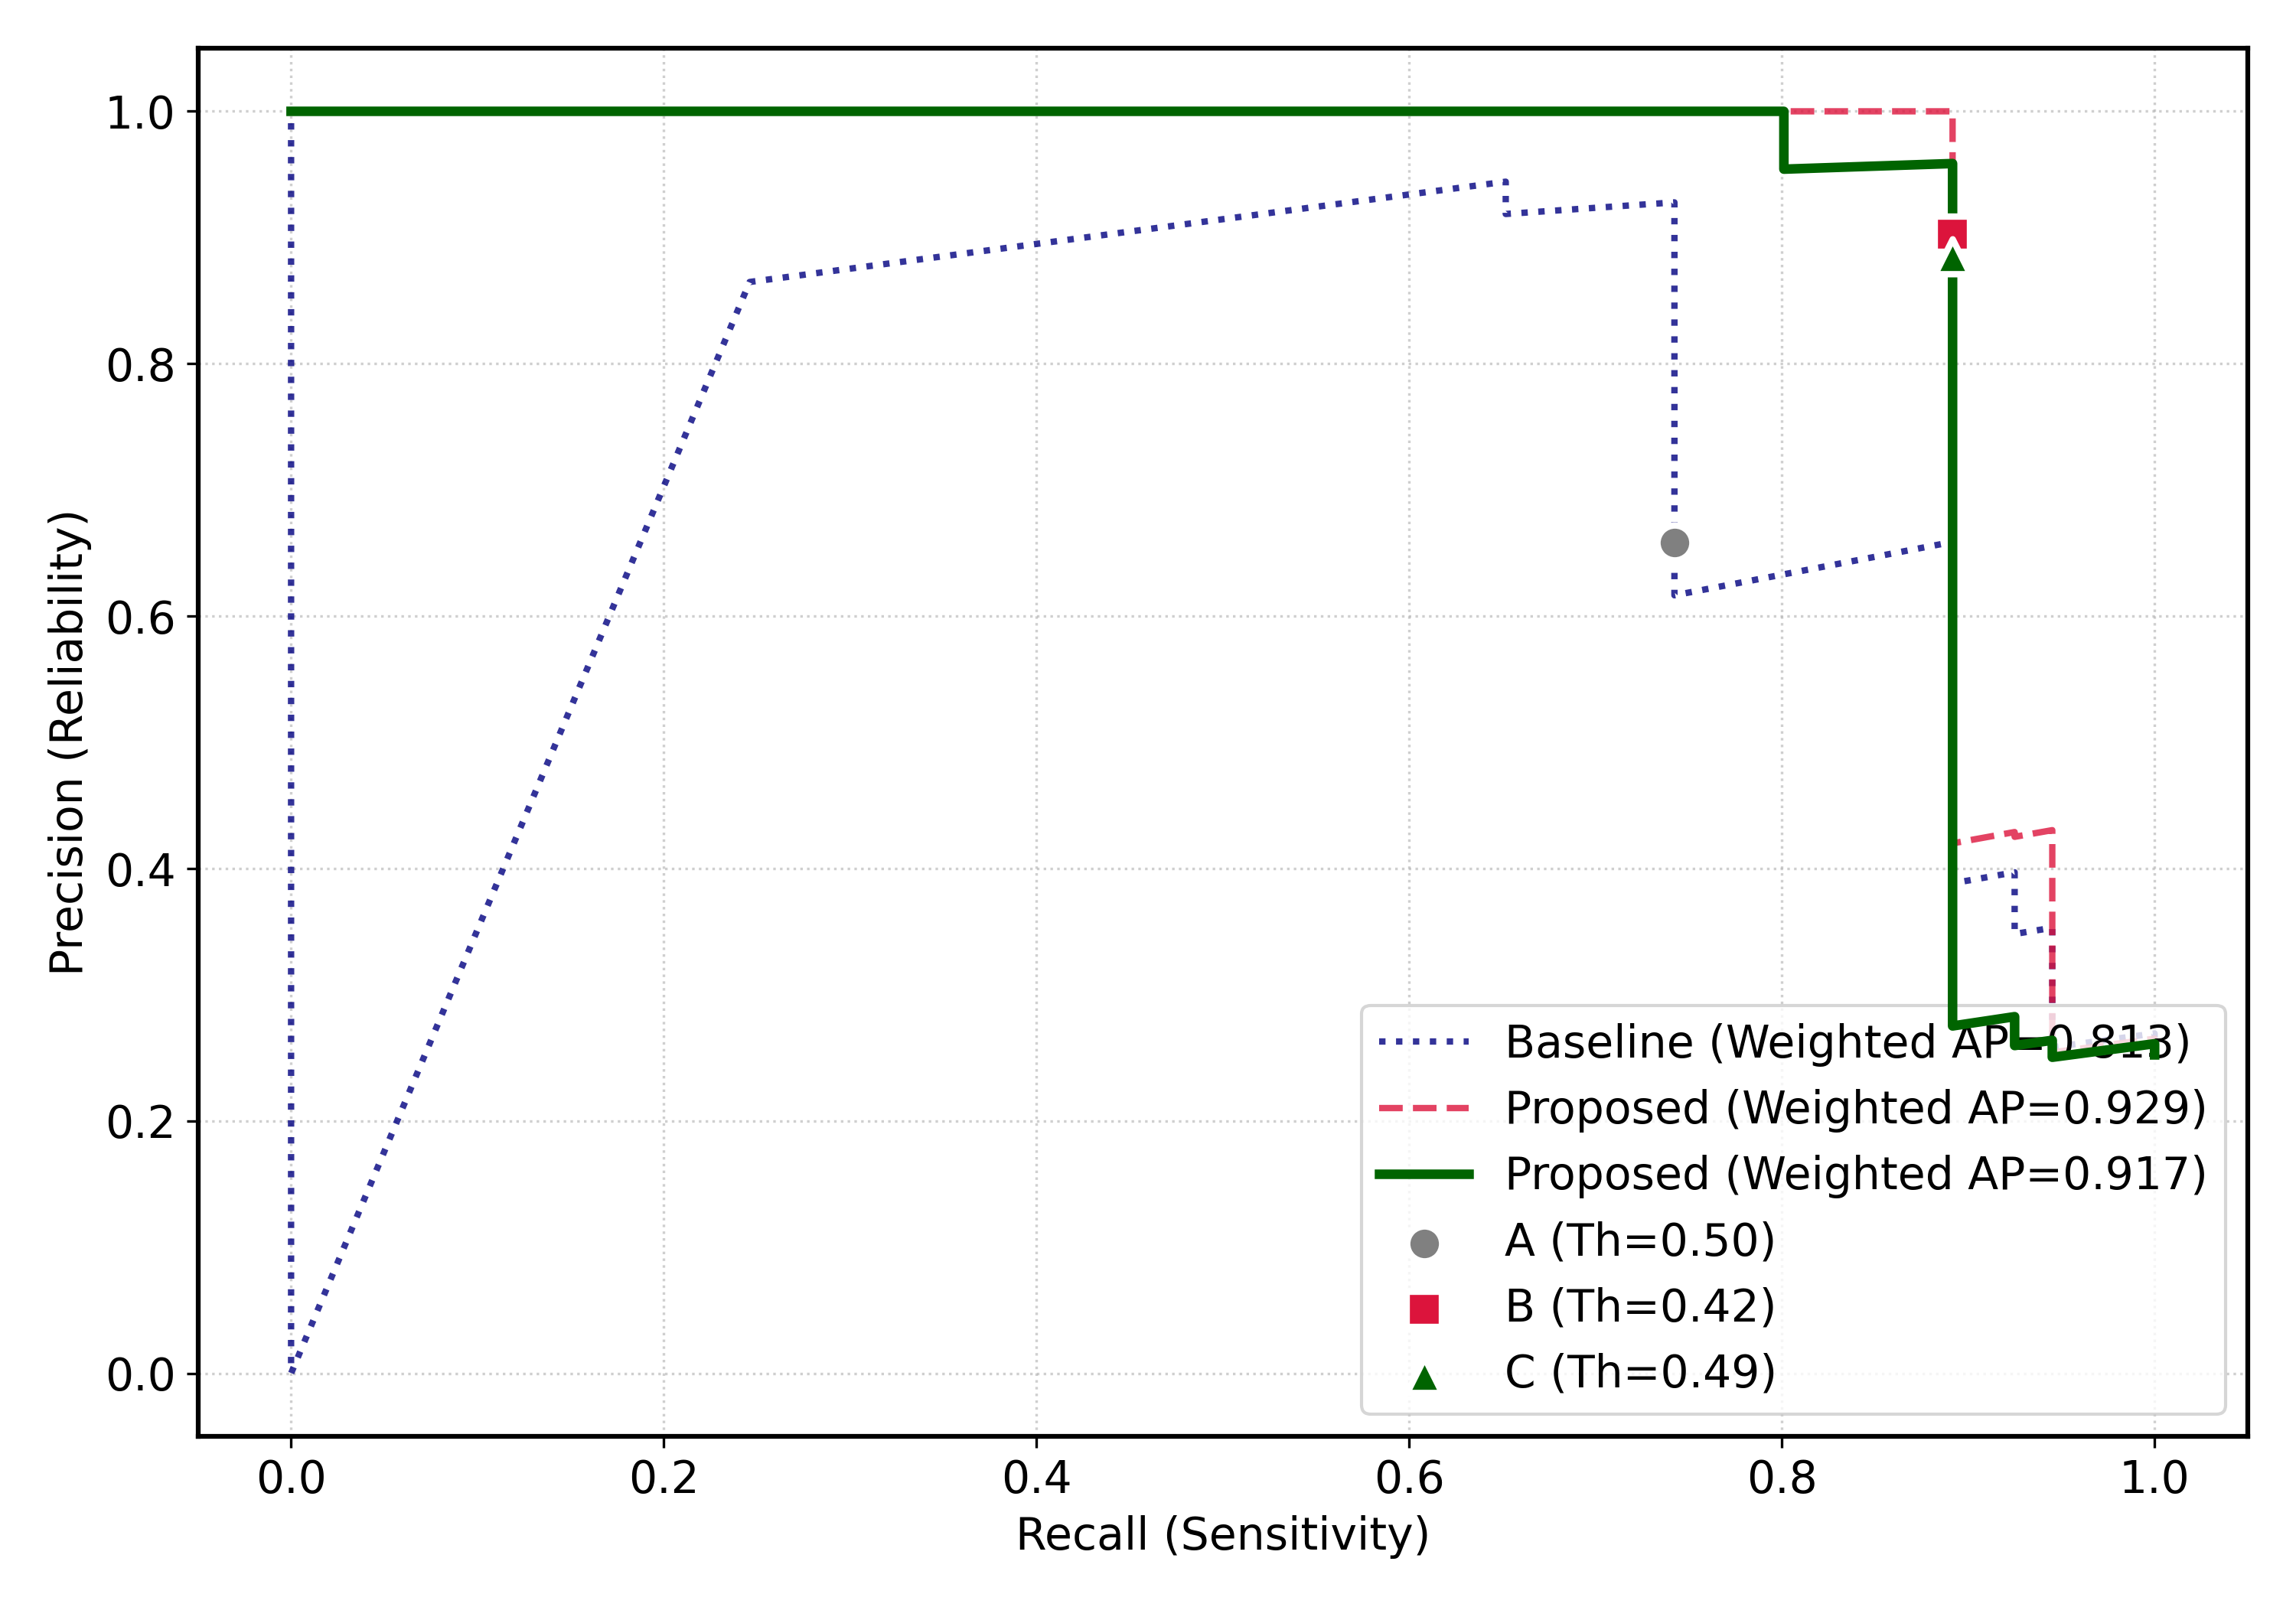
\includegraphics[width=\linewidth]{figures/fig_5_5b_pr(weight)_index2_scenario1.png}
    \caption*{(d) Index 2 / Weighted PR}
  \end{minipage}
  
  \caption{シナリオ1（トランプ関税ショック期）のPR曲線。
  上段（インデックス1）：モデルCがモデルBを上回り、特に重み付けPR(b)で顕著。
  下段（インデックス2）：モデルBがモデルCを上回り、物理的ターゲットではRMT単体で十分であることを示唆。}
  \label{fig:pr_scenario1}
\end{figure}

結果として、ターゲットと評価方法の組み合わせにより、以下の対照的な現象が観測された。

\begin{enumerate}
    \item \textbf{Index 1 における Model C の優位性 (a)(b):}
    経済指標をターゲットとした場合、通常評価(a)・重み付け評価(b)ともに、エネルギー項を追加した Model C（赤線）が Model B（青線）を上回った。特に(b)重み付け評価においてその差が顕著であり、エネルギー特徴量が「小規模なノイズ」と「致命的な下落」を選別するフィルタとして機能し、経済指標特有のダマシを抑制していることがわかる。

    \item \textbf{Index 2 における Model B の逆転 (c)(d):}
    一方、インパクト指標をターゲットとした場合、むしろ RMTのみを用いた Model B が最も高いAUCを示した。Model C は特に(d)重み付け評価において適合率の低下が見られ、ターゲット自体が物理的（非線形）である場合、入力特徴量に同様の物理量を加えることが、情報の重複による過学習やシグナルの相殺を招いた可能性が示唆される。
\end{enumerate}

\subsubsection{Scenario 2: 植田ショック～トランプ期における評価}
次に、検証期間を「Scenario 2（2024/3/1 -- 2025/6/30）」に拡張し、異なる相場環境（レジーム）を含む長期間におけるモデルのロバスト性を検証する。

図\ref{fig:pr_scenario2}に、Scenario 2 におけるPR曲線を示す。

\begin{figure}[H]
  \centering
  % --- 上段: Index 1 ---
  \begin{minipage}[b]{0.48\linewidth}
    \centering
    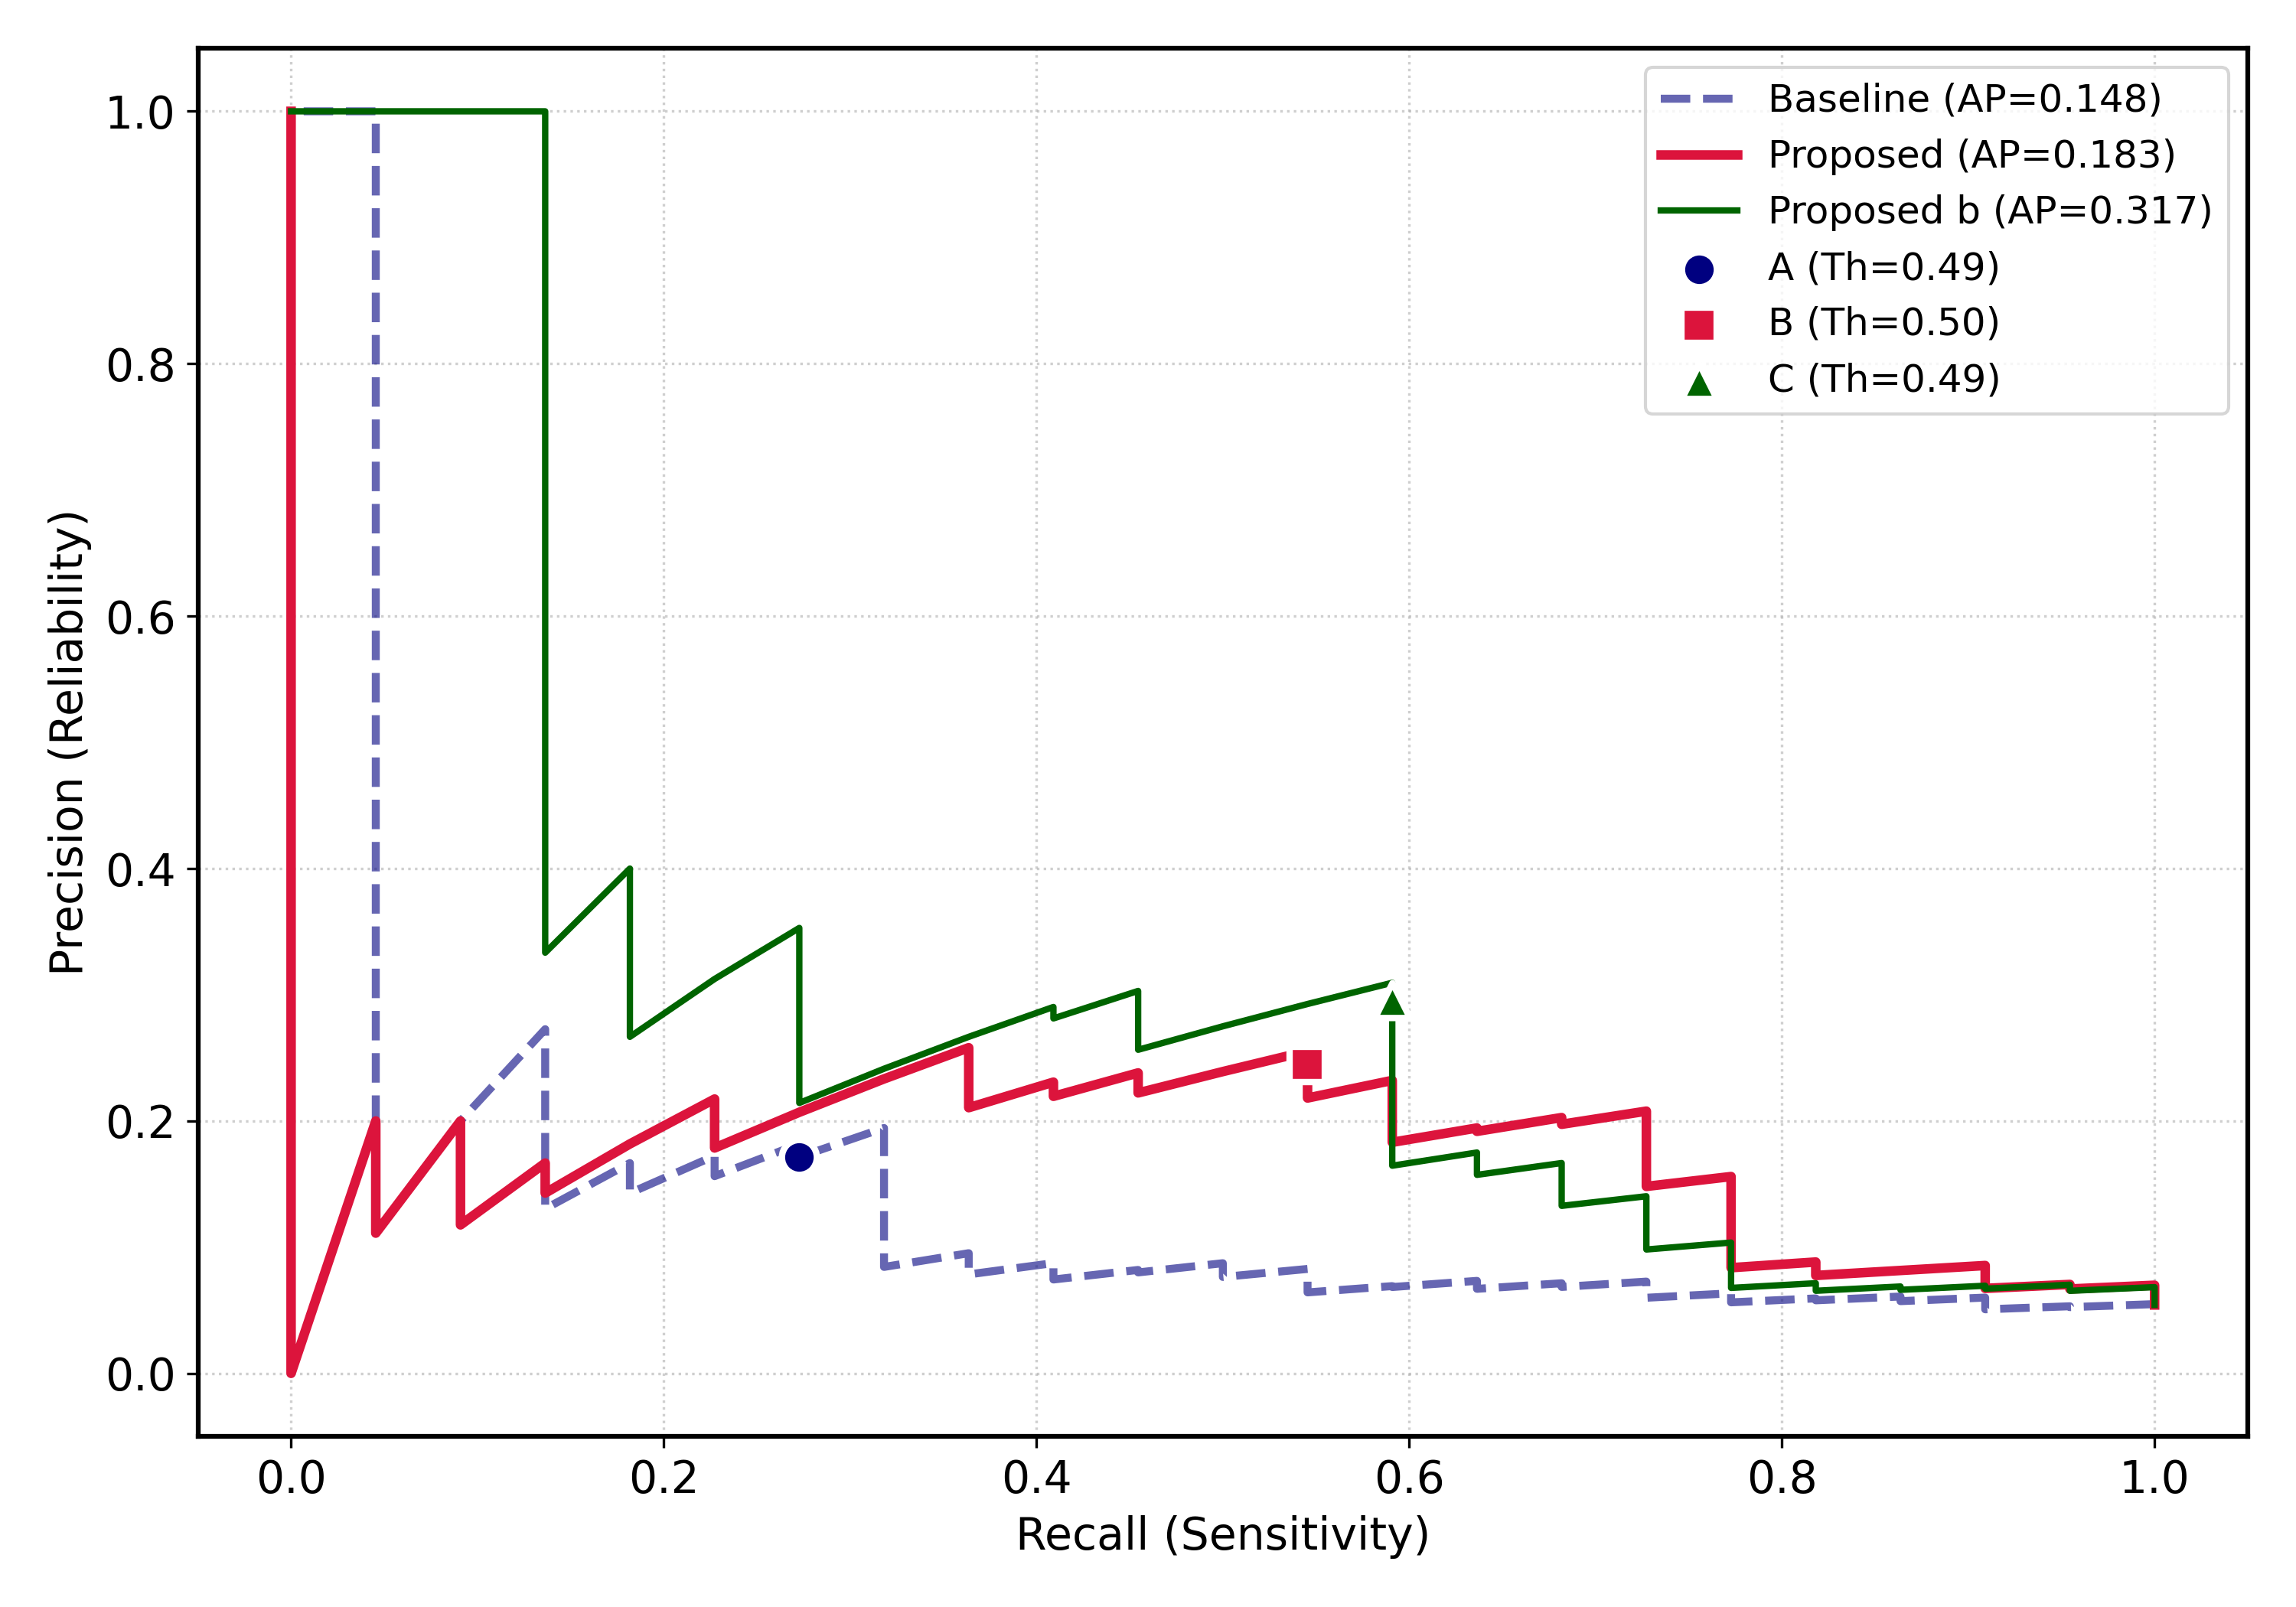
\includegraphics[width=\linewidth]{figures/fig_5_6a_pr(normal)_index1_scenario2.png}
    \caption*{(a) Index 1 / Normal PR}
  \end{minipage}
  \begin{minipage}[b]{0.48\linewidth}
    \centering
    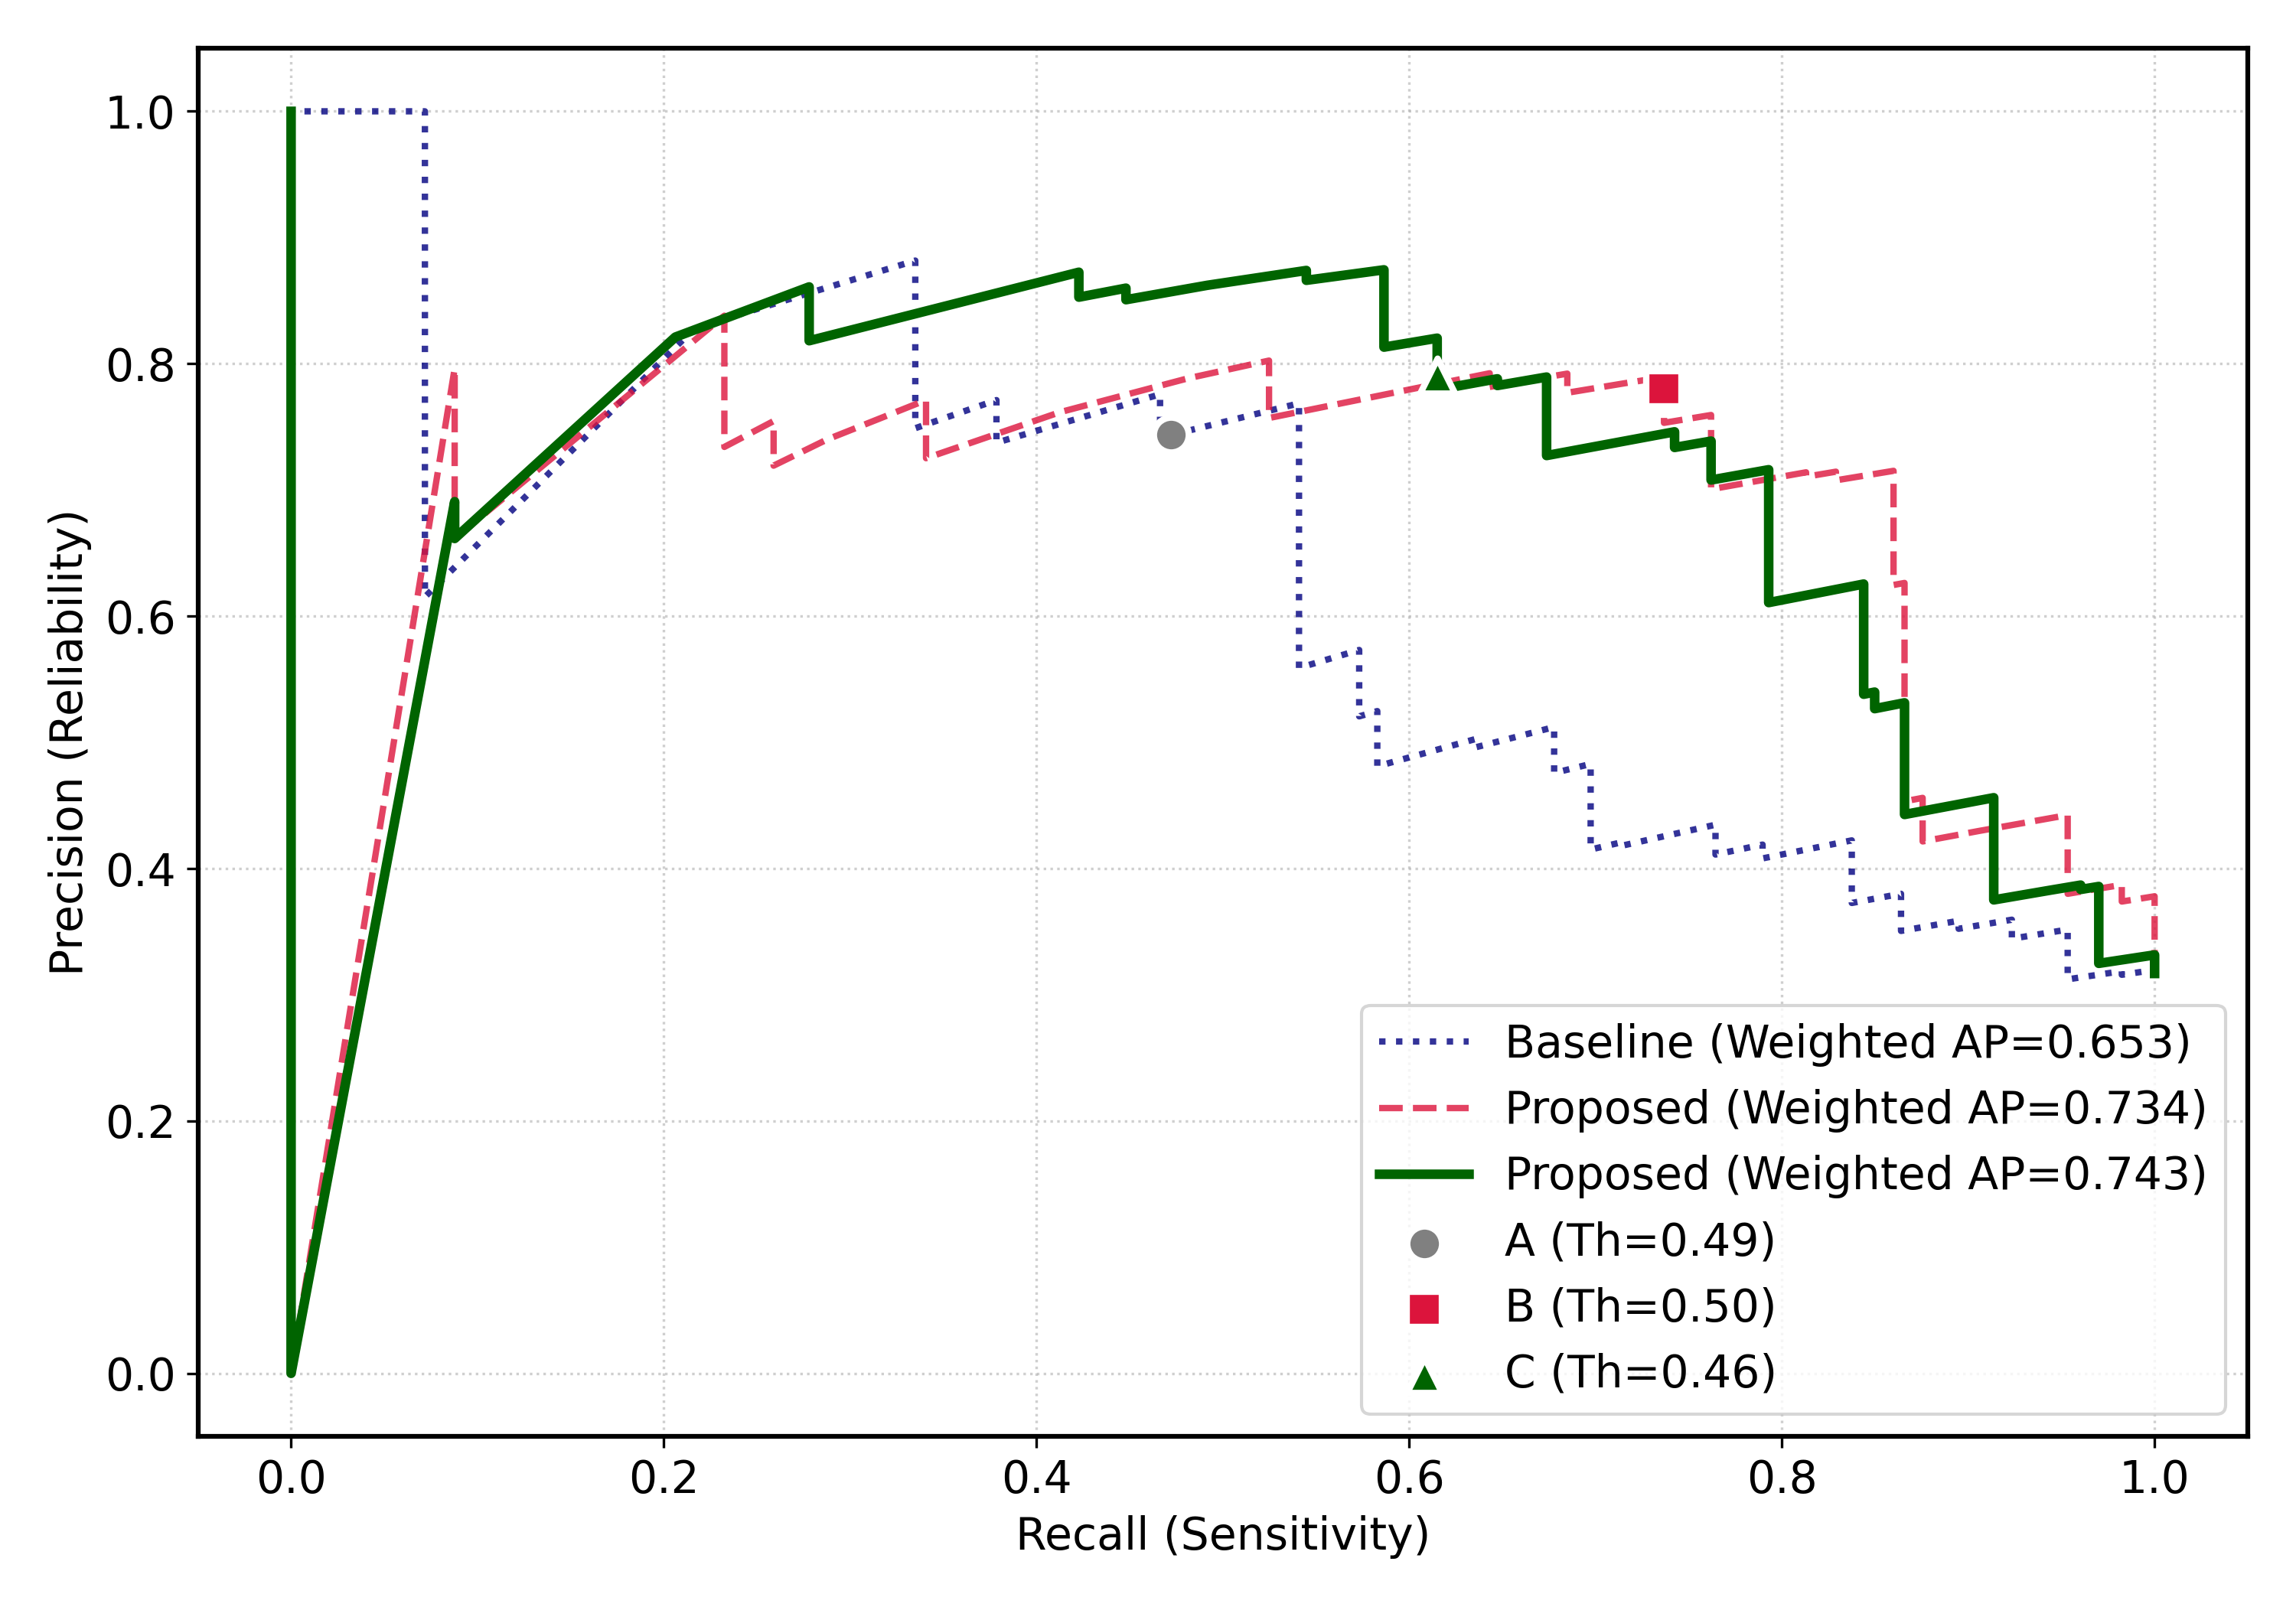
\includegraphics[width=\linewidth]{figures/fig_5_6b_pr(weight)_index1_scenario2.png}
    \caption*{(b) Index 1 / Weighted PR}
  \end{minipage}

  \vspace{0.5cm}
  
  % --- 下段: Index 2 ---
  \begin{minipage}[b]{0.48\linewidth}
    \centering
    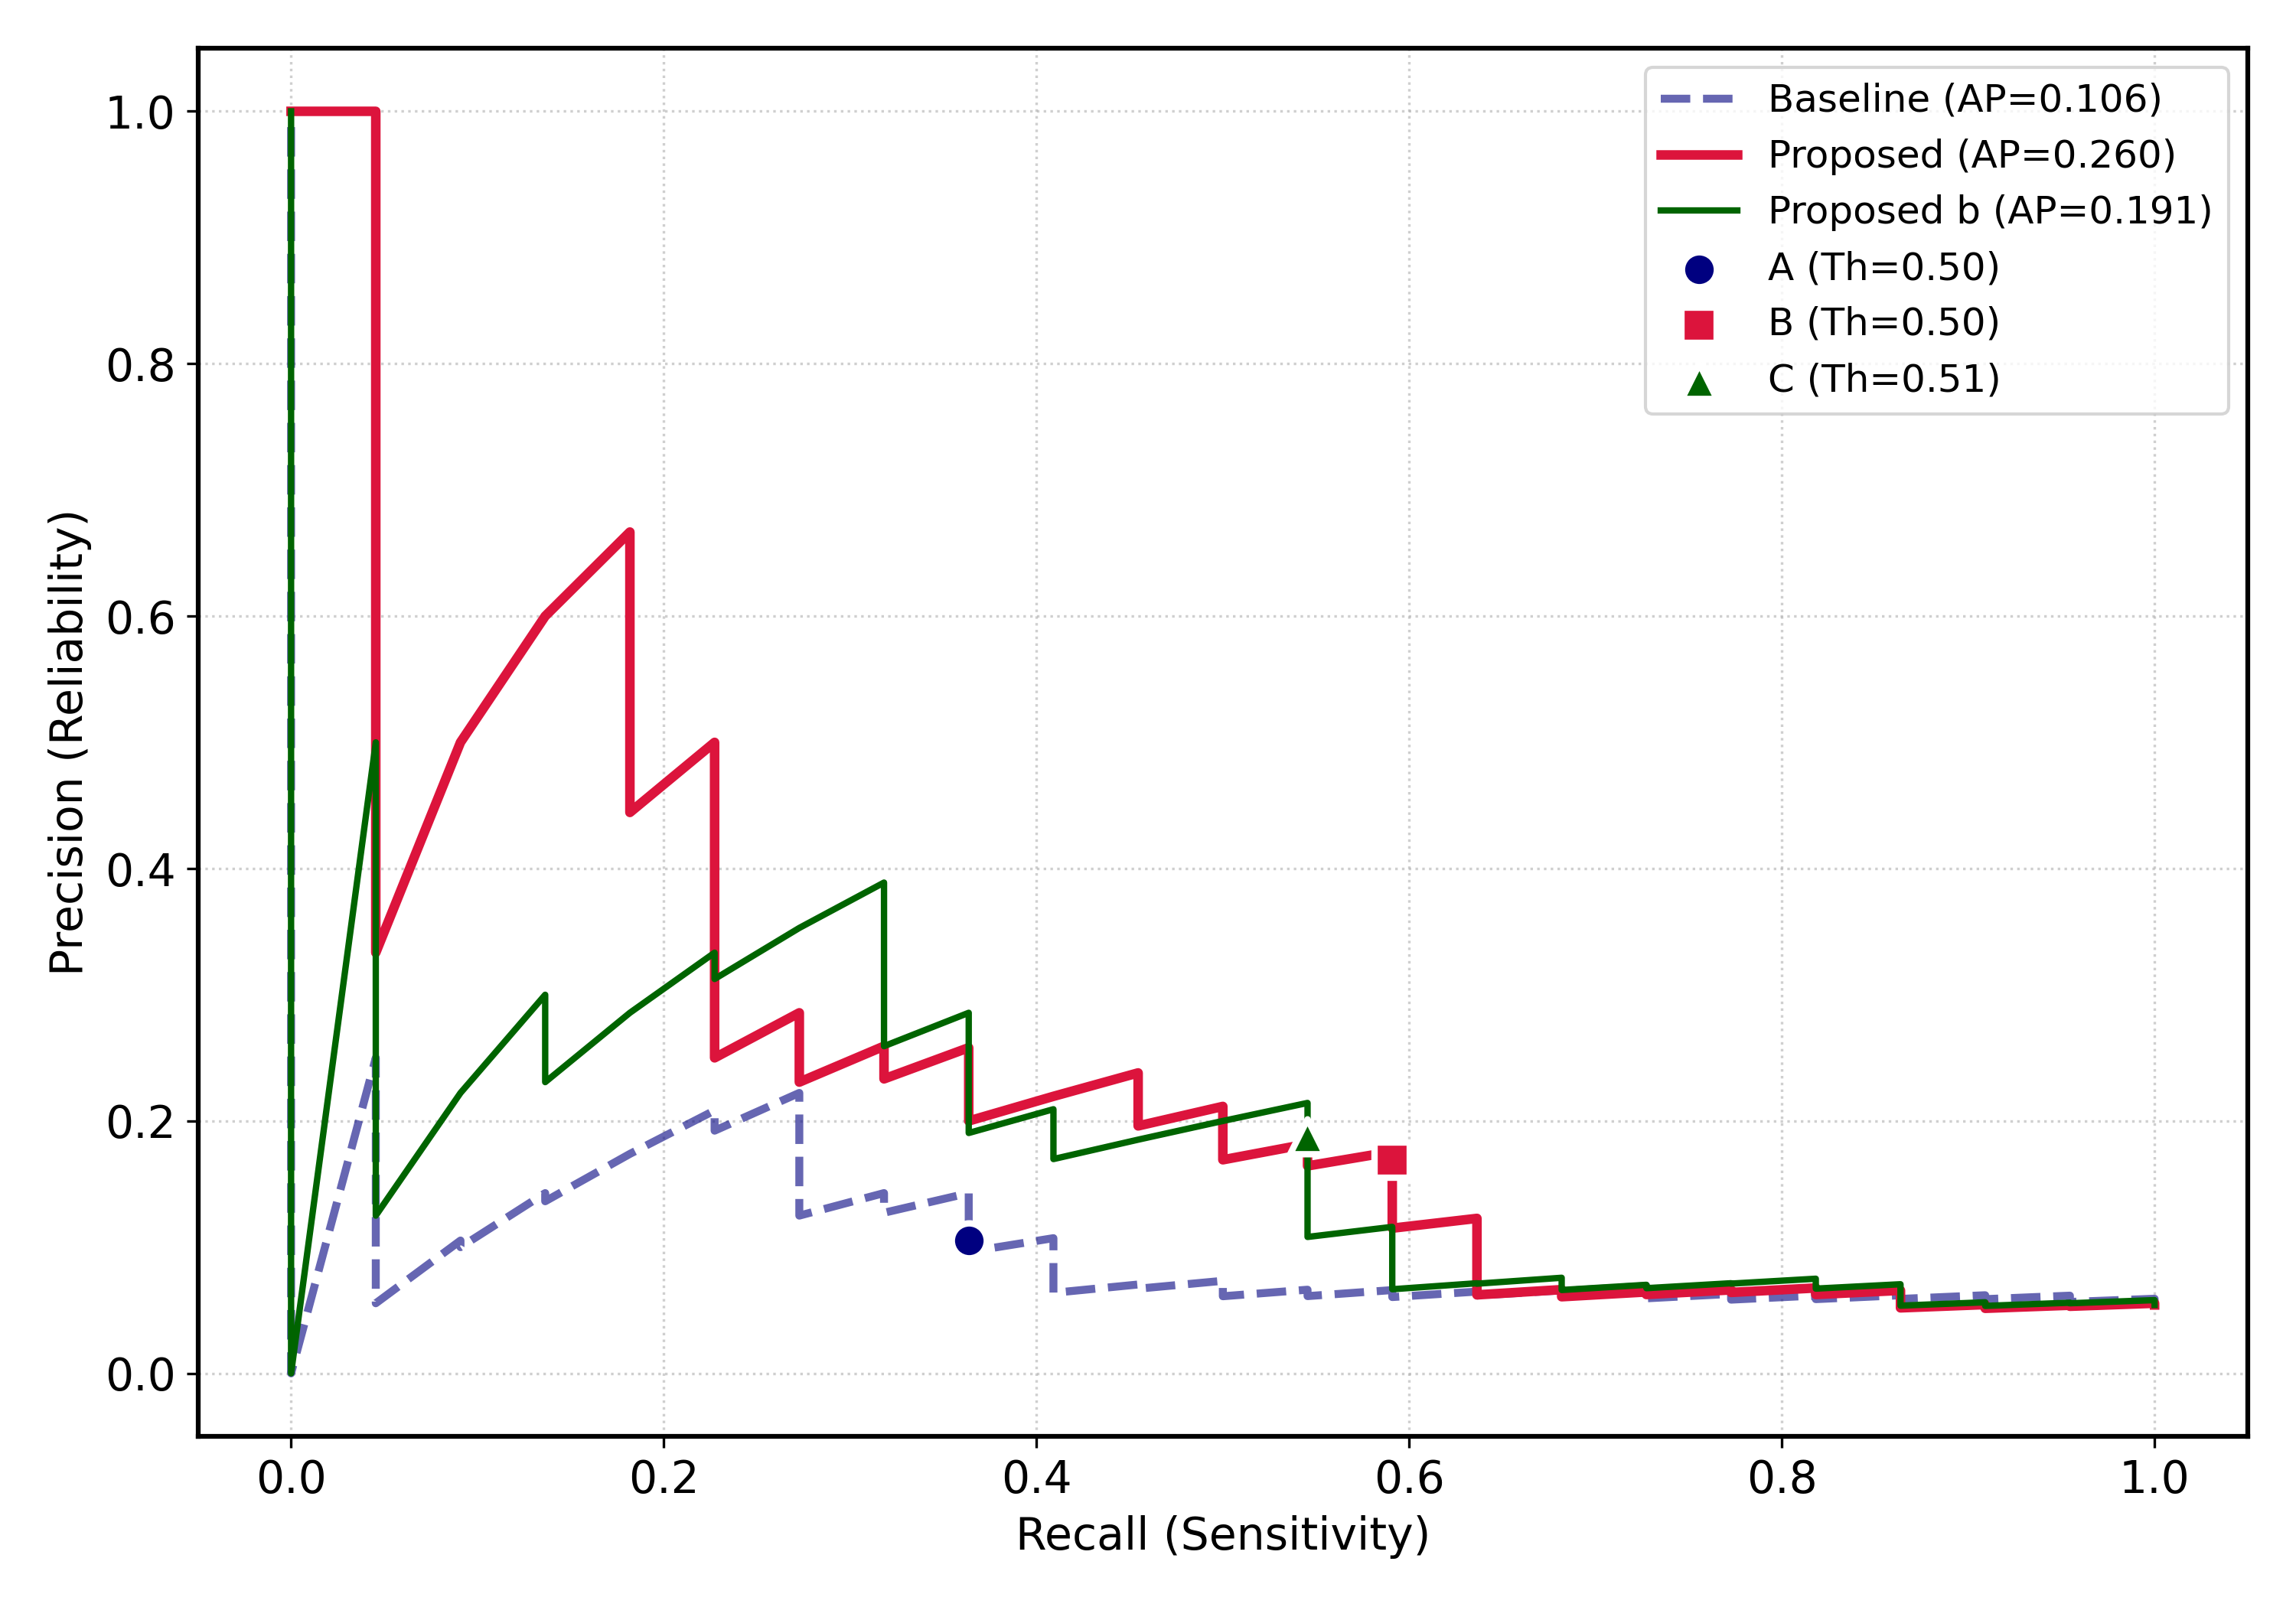
\includegraphics[width=\linewidth]{figures/fig_5_7a_pr(normal)_index2_scenario2.png}
    \caption*{(c) Index 2 / Normal PR}
  \end{minipage}
  \begin{minipage}[b]{0.48\linewidth}
    \centering
    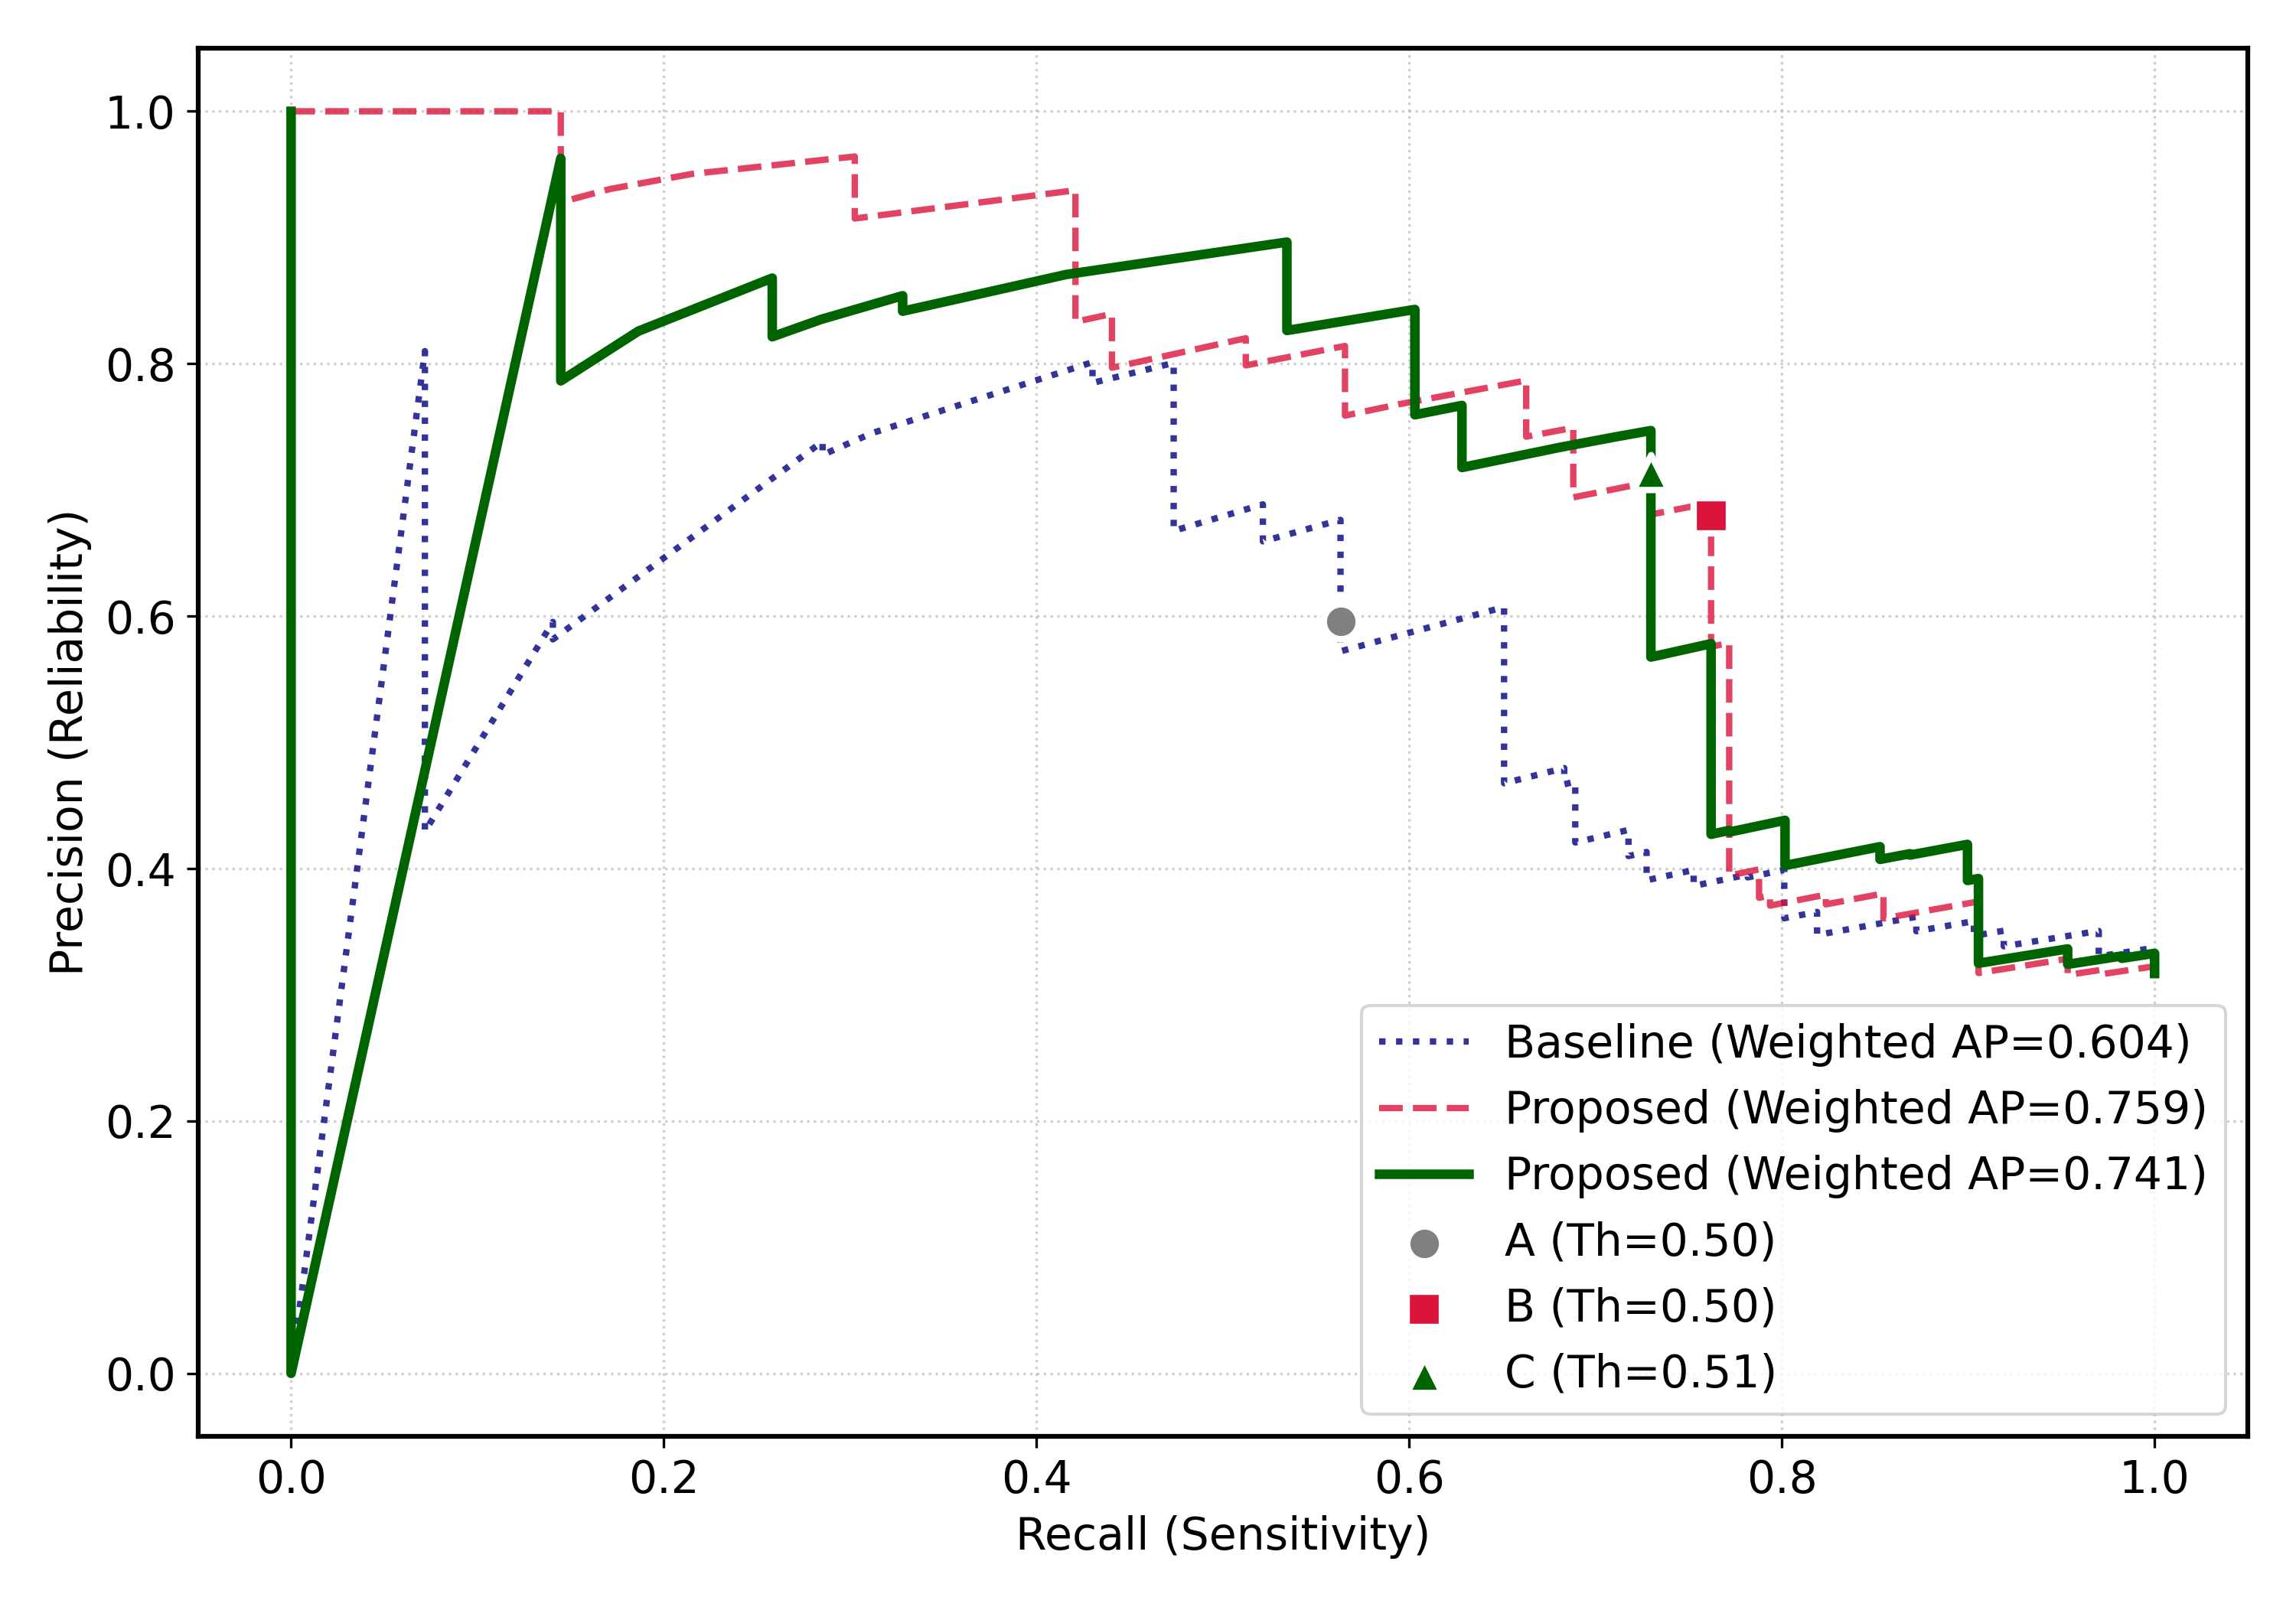
\includegraphics[width=\linewidth]{figures/fig_5_7b_pr(weight)_index2_scenario2.png}
    \caption*{(d) Index 2 / Weighted PR}
  \end{minipage}

  \caption{シナリオ2（植田ショック～トランプ期）のPR曲線。
  長期評価においても、Index 2 (d) における Model B の優位性は揺るがなかった。}
  \label{fig:pr_scenario2}
\end{figure}

長期評価においても、Scenario 1 と同様の傾向が確認された。特筆すべきは、Model A（テクニカル）がレジーム変化により大きく精度を落とす中で、Model B は安定して高い精度を維持している点である。これは、RMT特徴量が価格スケールに依存しない「定常性」を持つため、異なる相場環境下でもロバストに機能したことを示している。
一方、Model C は長期運用において精度の低下が見られた。これはエネルギー特徴量が時価総額 $M$ という「非定常」な成長変数を含むため、時間の経過とともに閾値がドリフトしたことが原因と考えられる。

\subsection{ミクロ評価：モデル判断の物理的解釈}
本節では、Index 2 において最も高い性能を示した Model B が、具体的にどのような物理現象を捉えているのかを、SHAP分析および時系列のミクロ挙動から解明する。

\subsubsection{SHAP分析による大域的解釈}
図\ref{fig:shap_scenario1}に、Scenario 1 における各モデルの SHAP Summary Plot を示す。

\begin{figure}[htbp]
  \centering
  % Index 1 のSHAP比較
  \begin{minipage}[b]{0.48\linewidth}
    \centering
    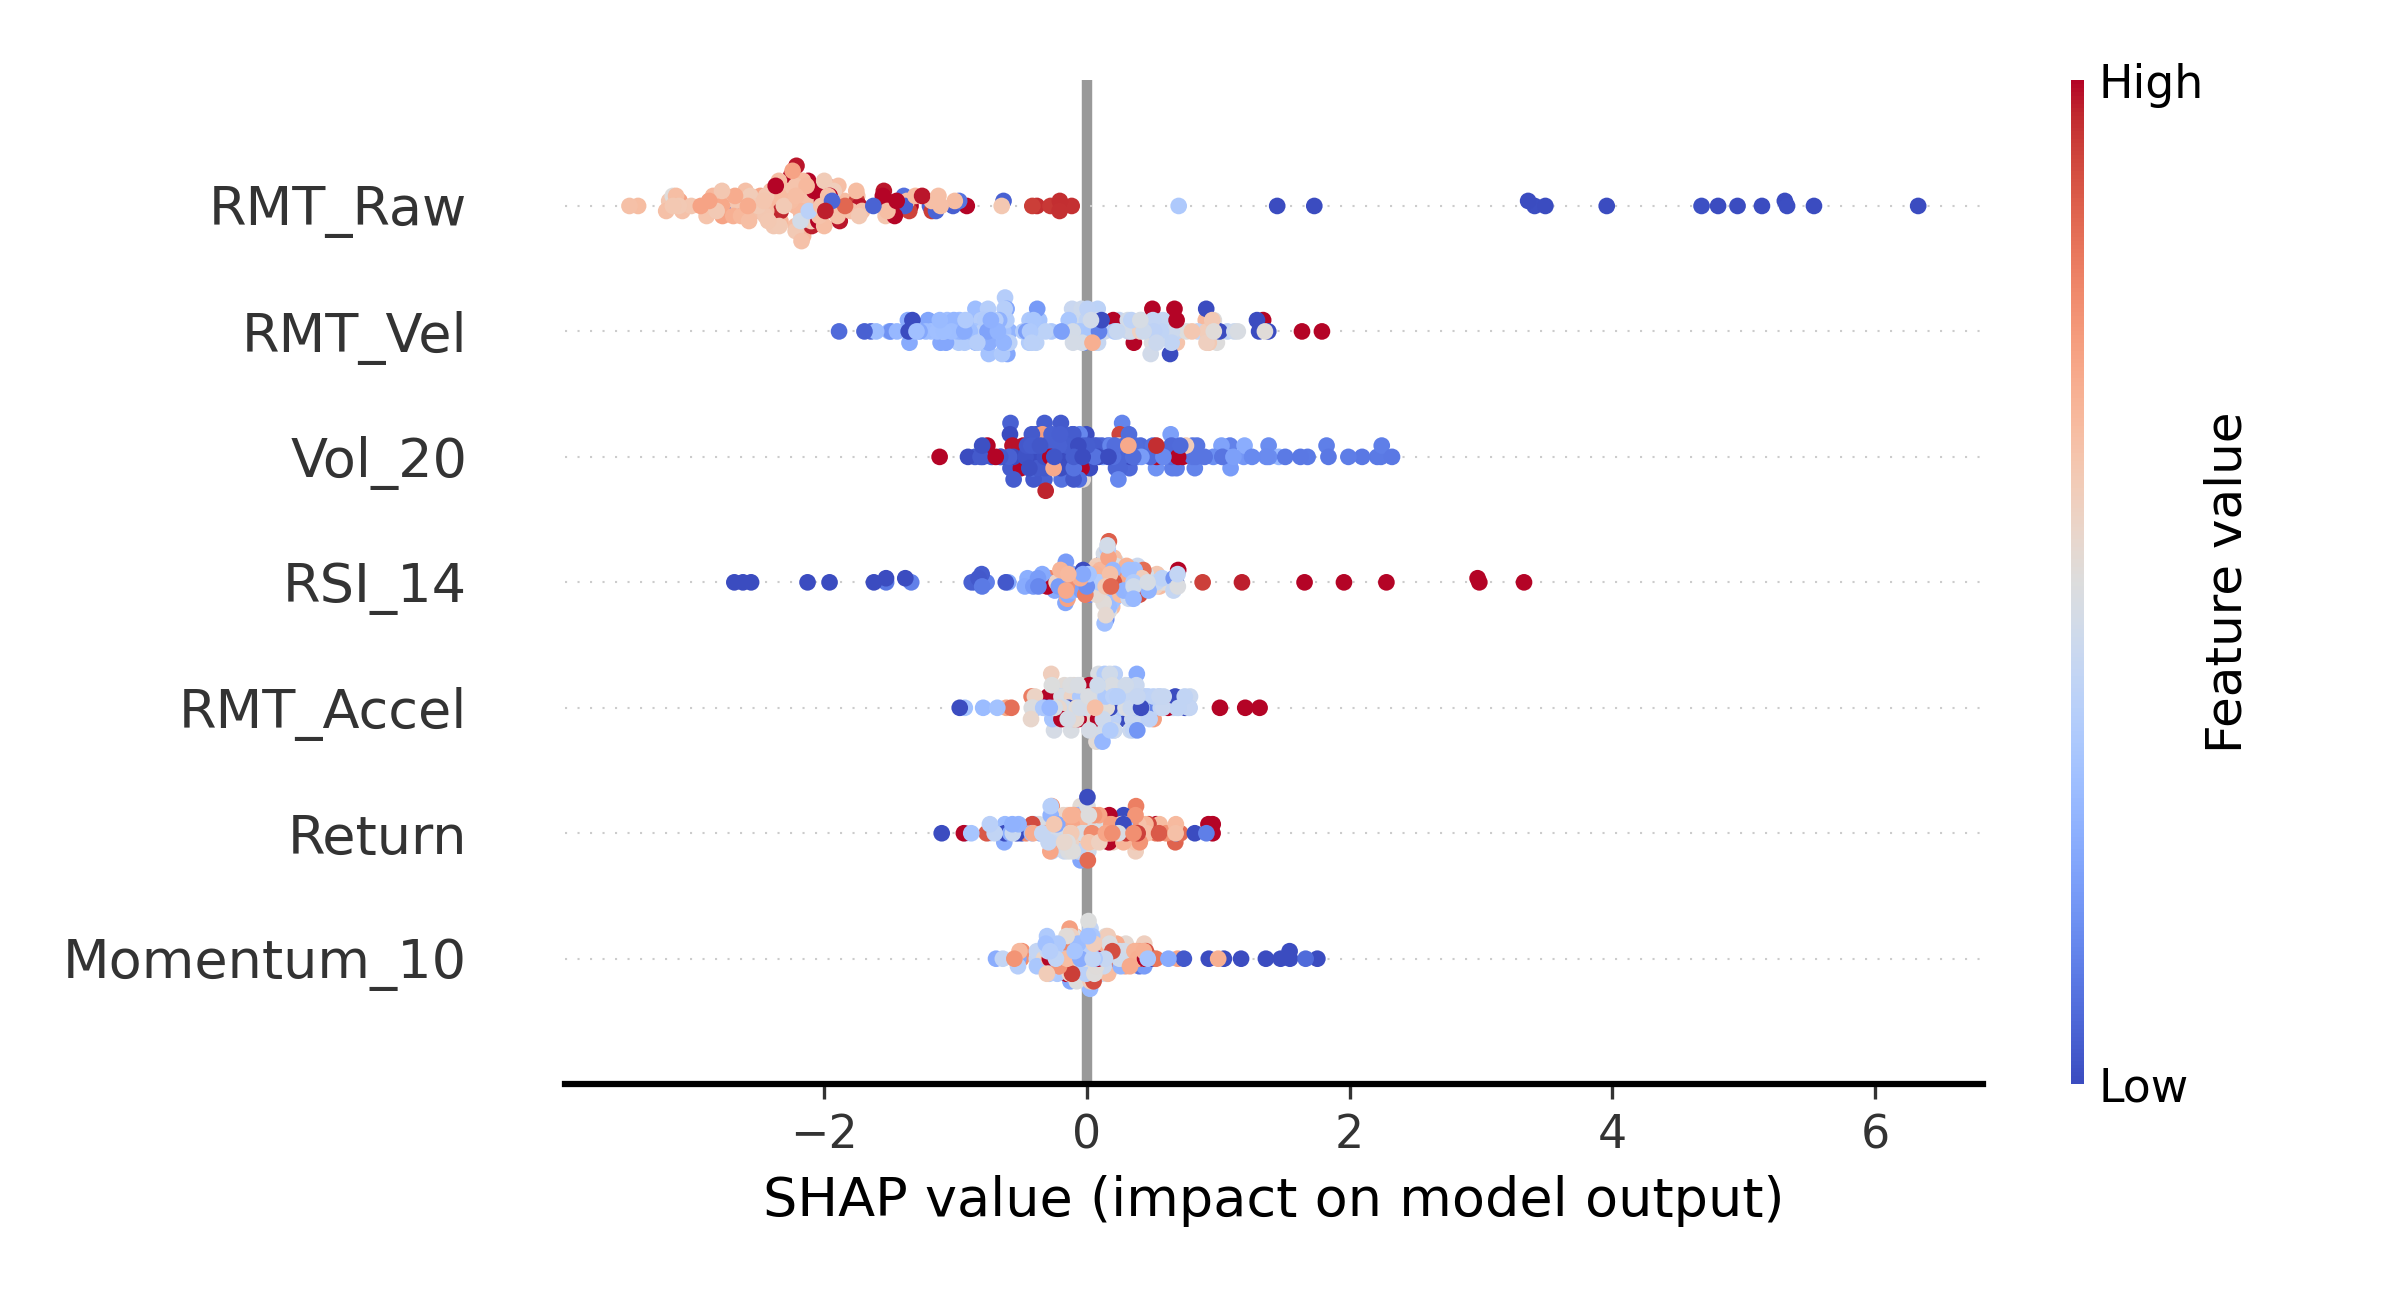
\includegraphics[width=\linewidth]{figures/fig_5_8a_shap_modelB_index1_scenario1.png}
    \caption*{(a) Index 1 / Model B}
  \end{minipage}
  \begin{minipage}[b]{0.48\linewidth}
    \centering
    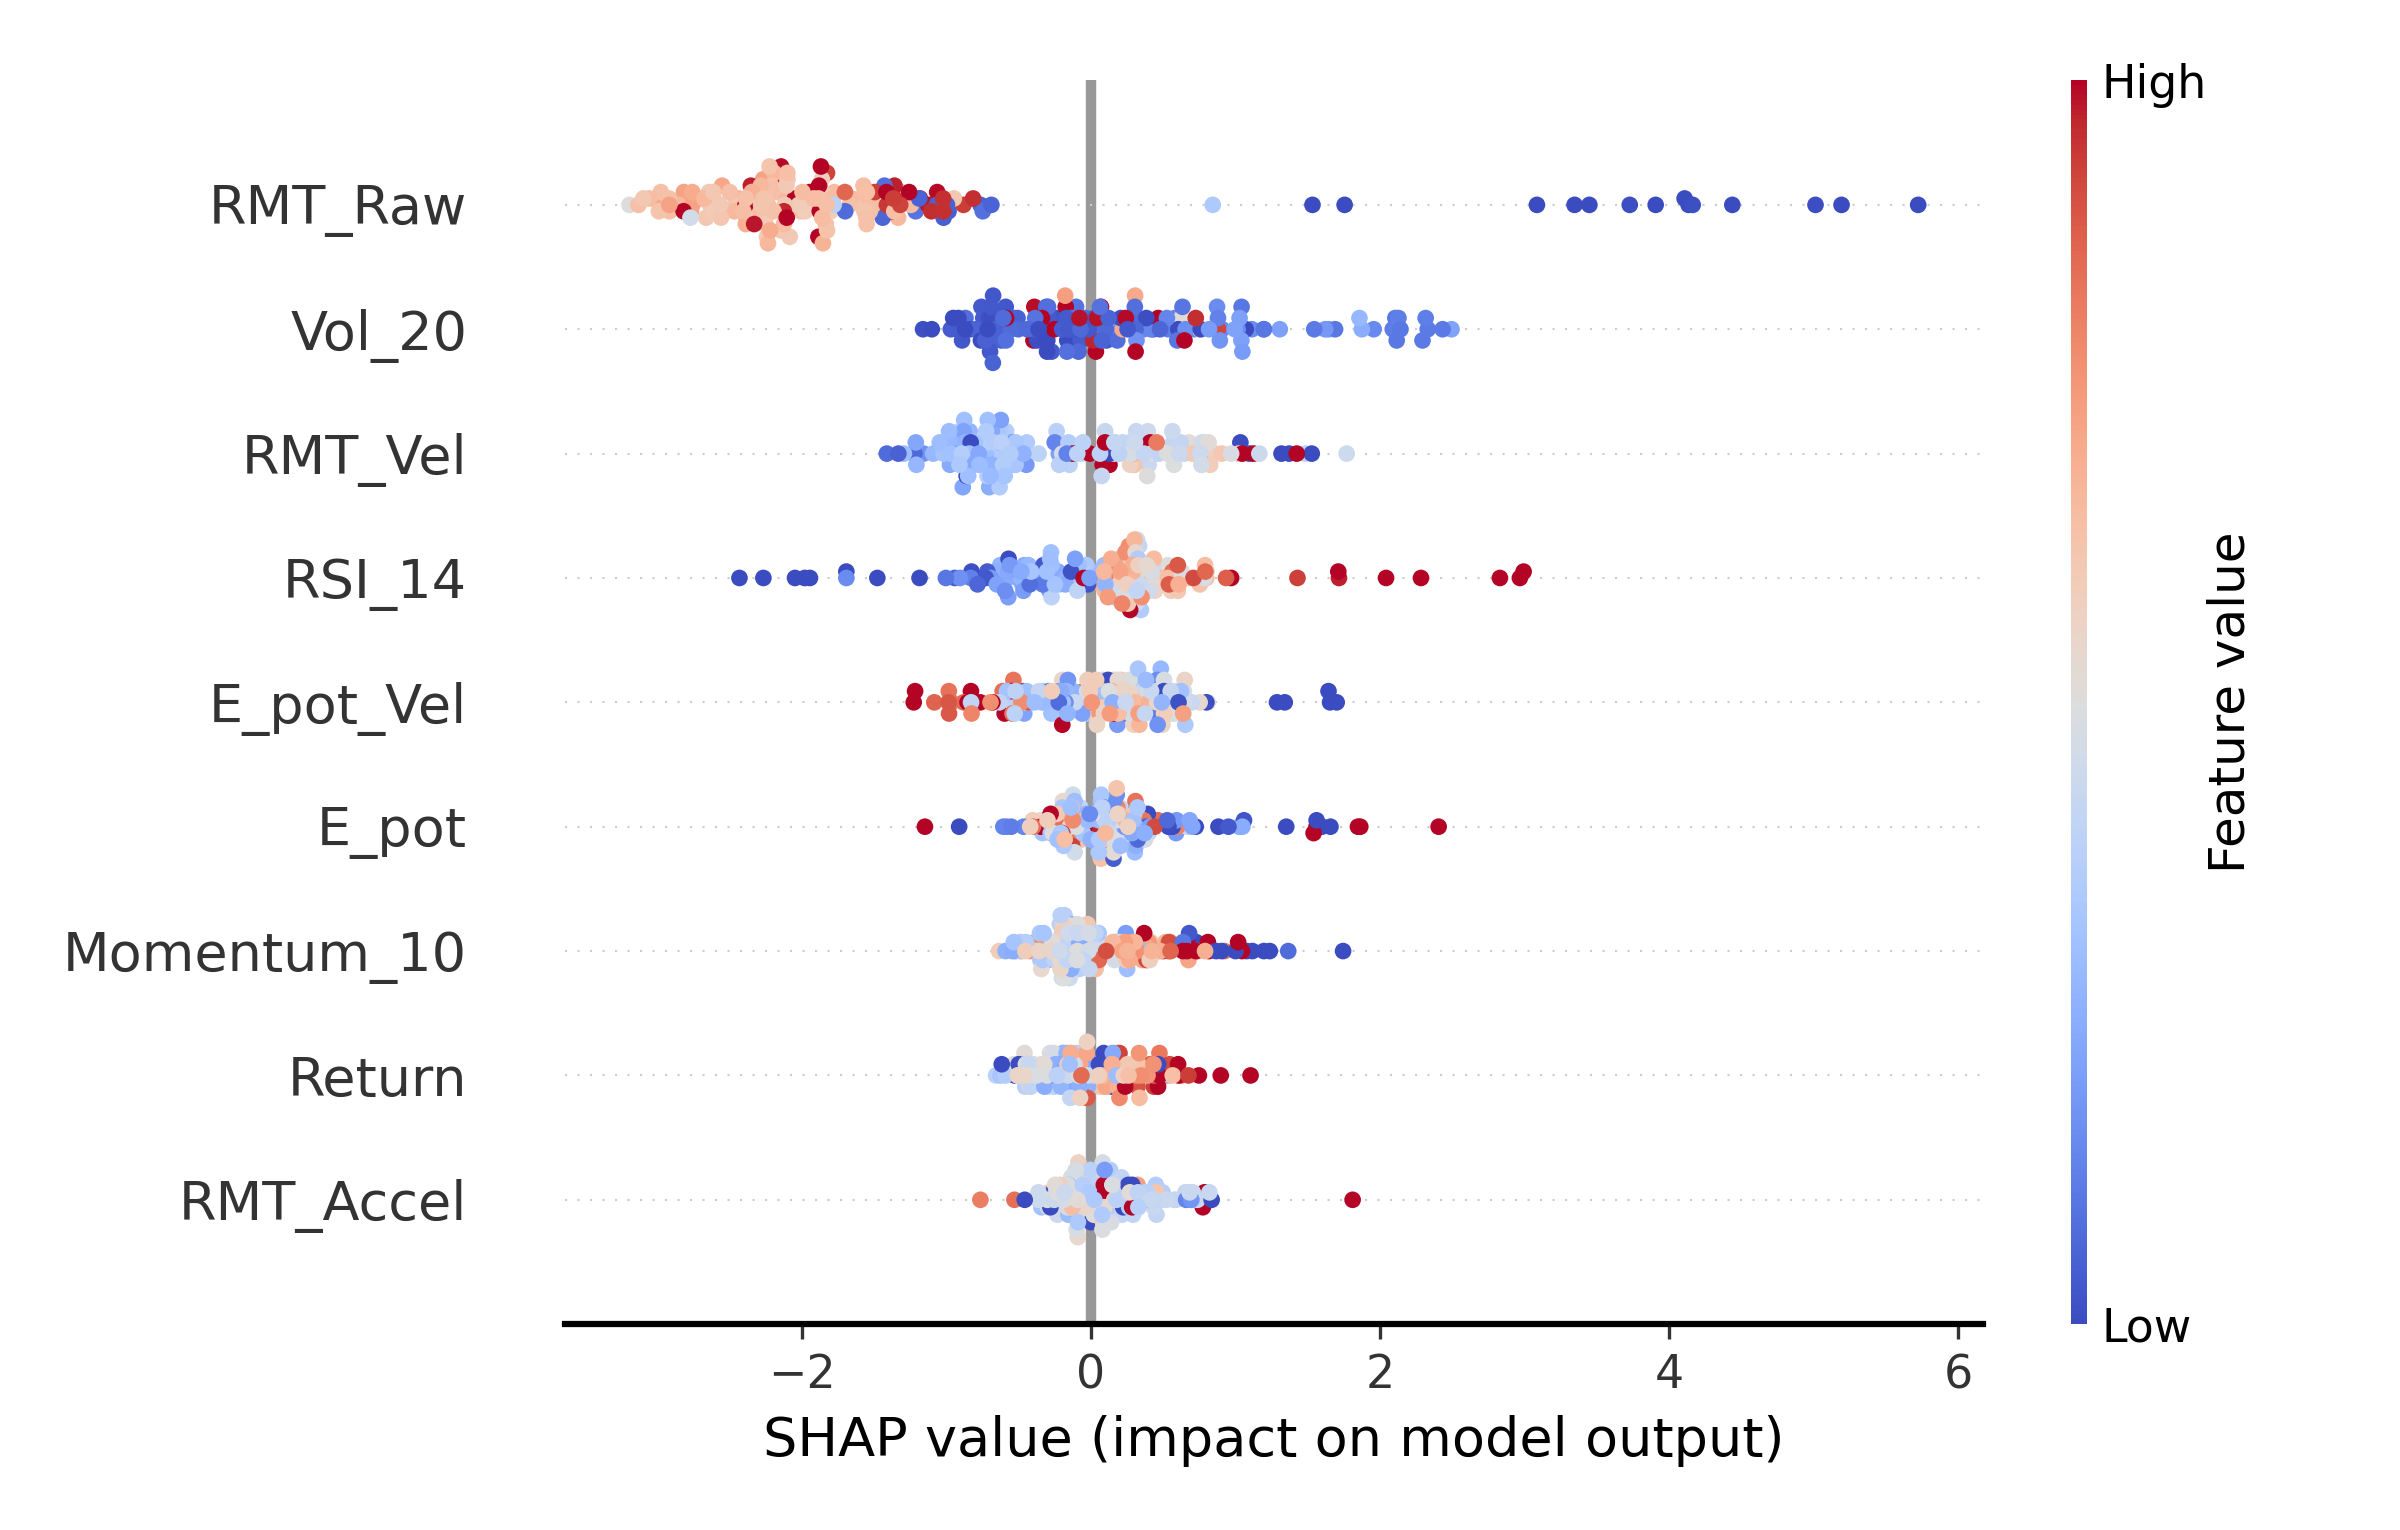
\includegraphics[width=\linewidth]{figures/fig_5_8b_shap_modelC_index1_scenario1.png}
    \caption*{(b) Index 1 / Model C}
  \end{minipage}
  
  \vspace{0.5cm}
  
  % Index 2 のSHAP比較
  \begin{minipage}[b]{0.48\linewidth}
    \centering
    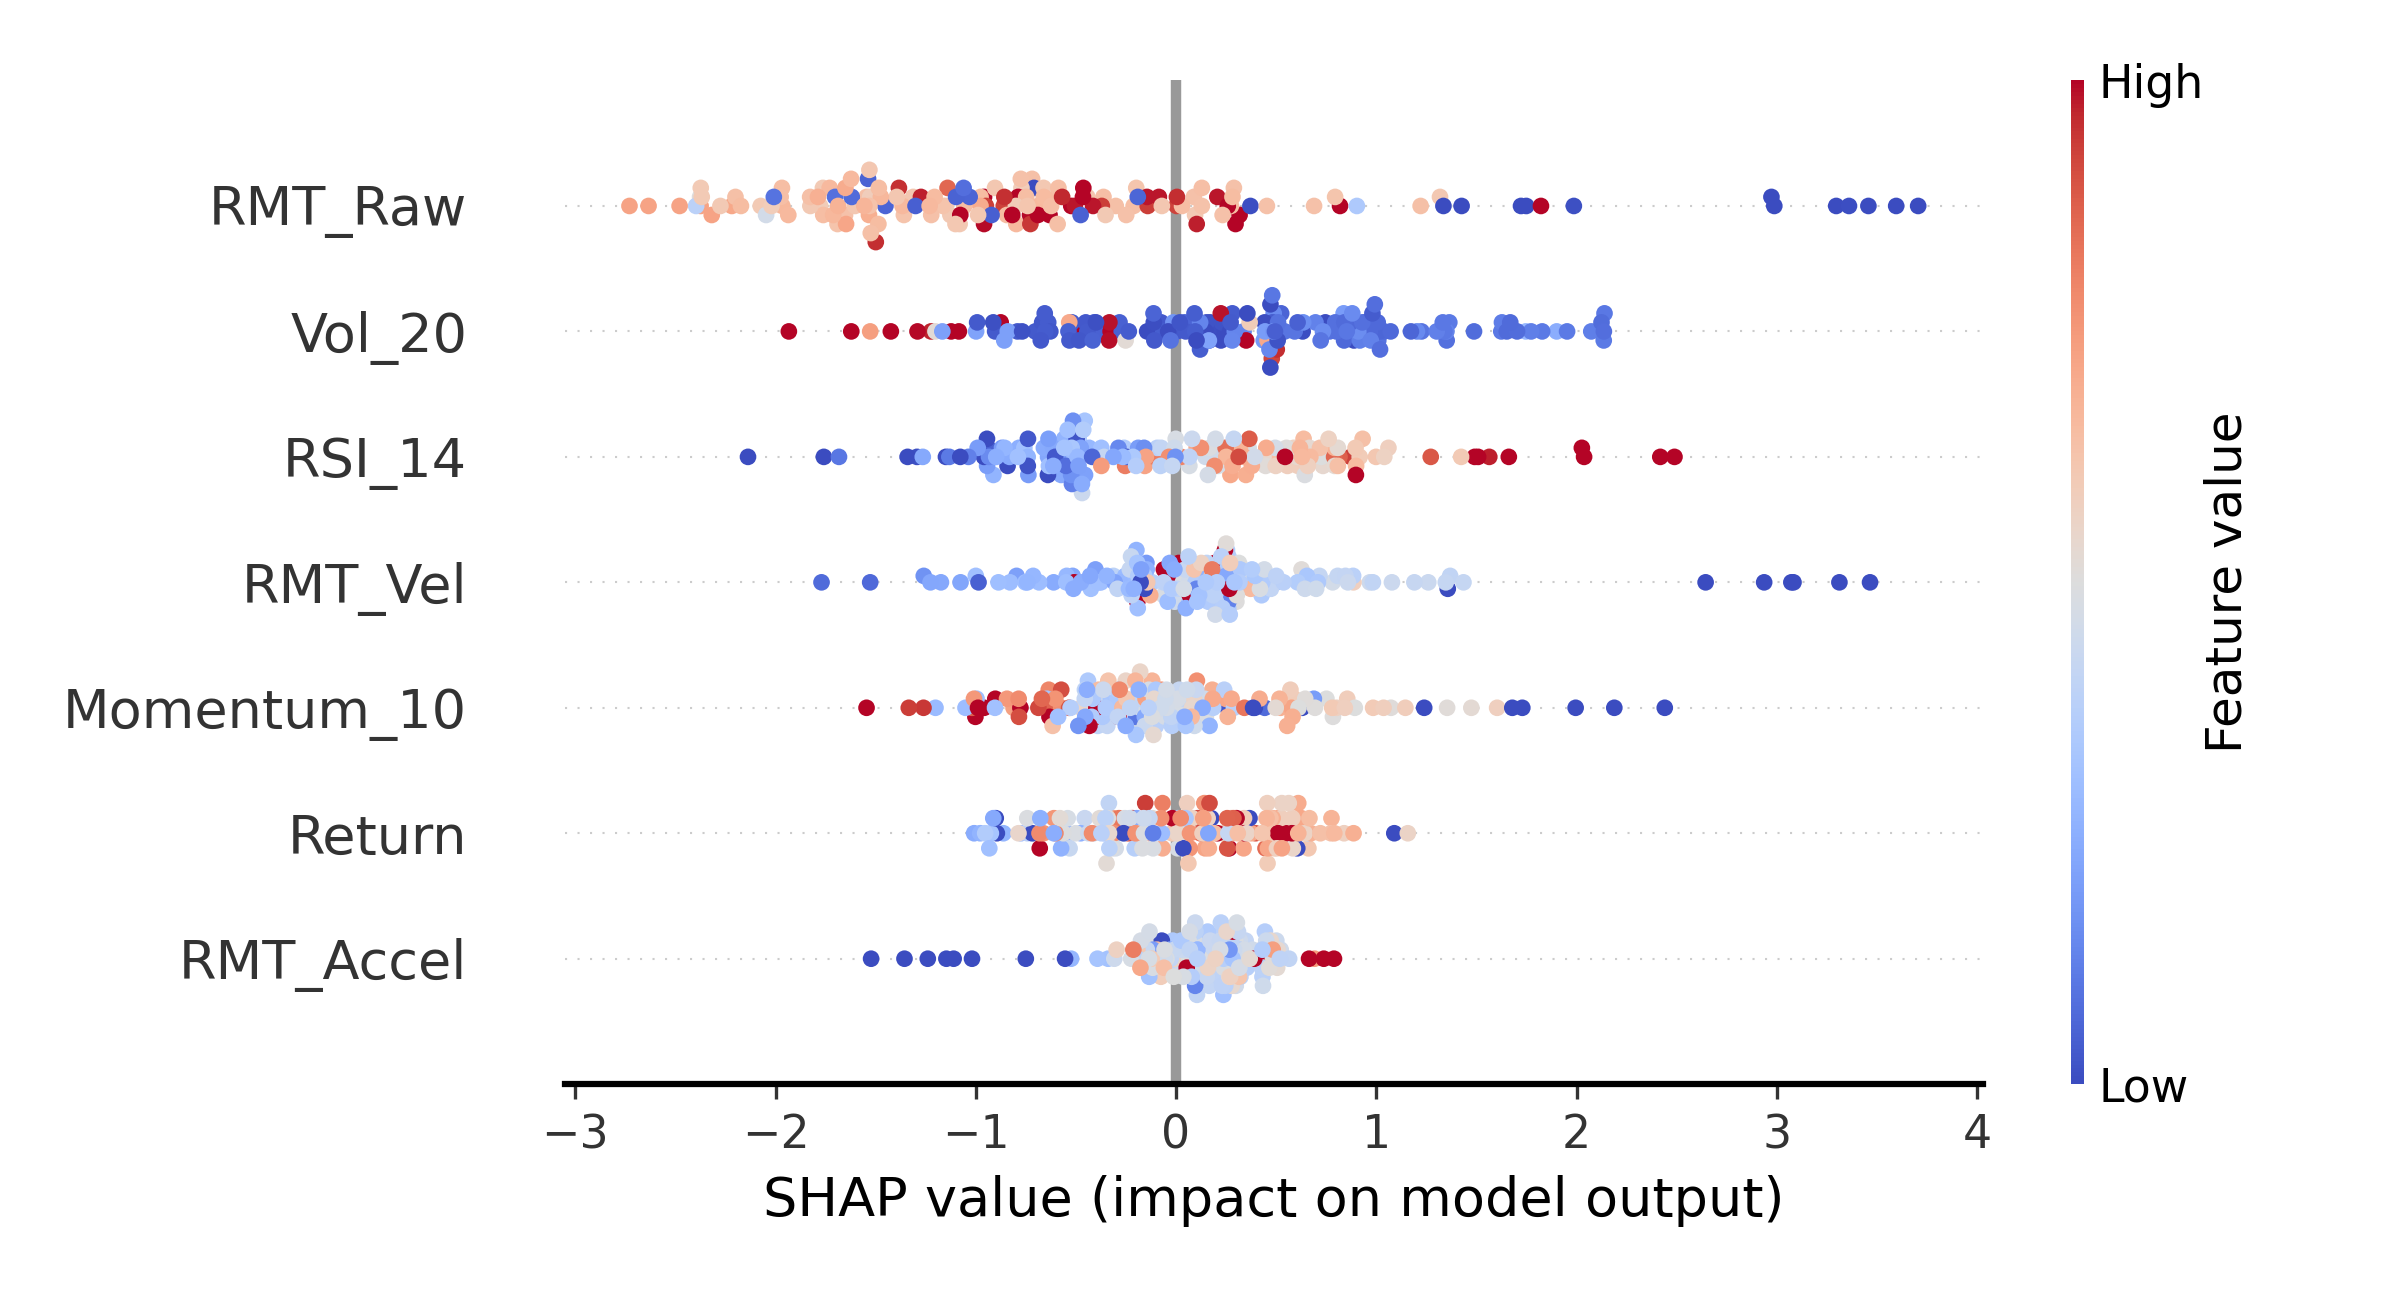
\includegraphics[width=\linewidth]{figures/fig_5_9a_shap_modelB_index2_scenario1.png}
    \caption*{(c) Index 2 / Model B}
  \end{minipage}
  \begin{minipage}[b]{0.48\linewidth}
    \centering
    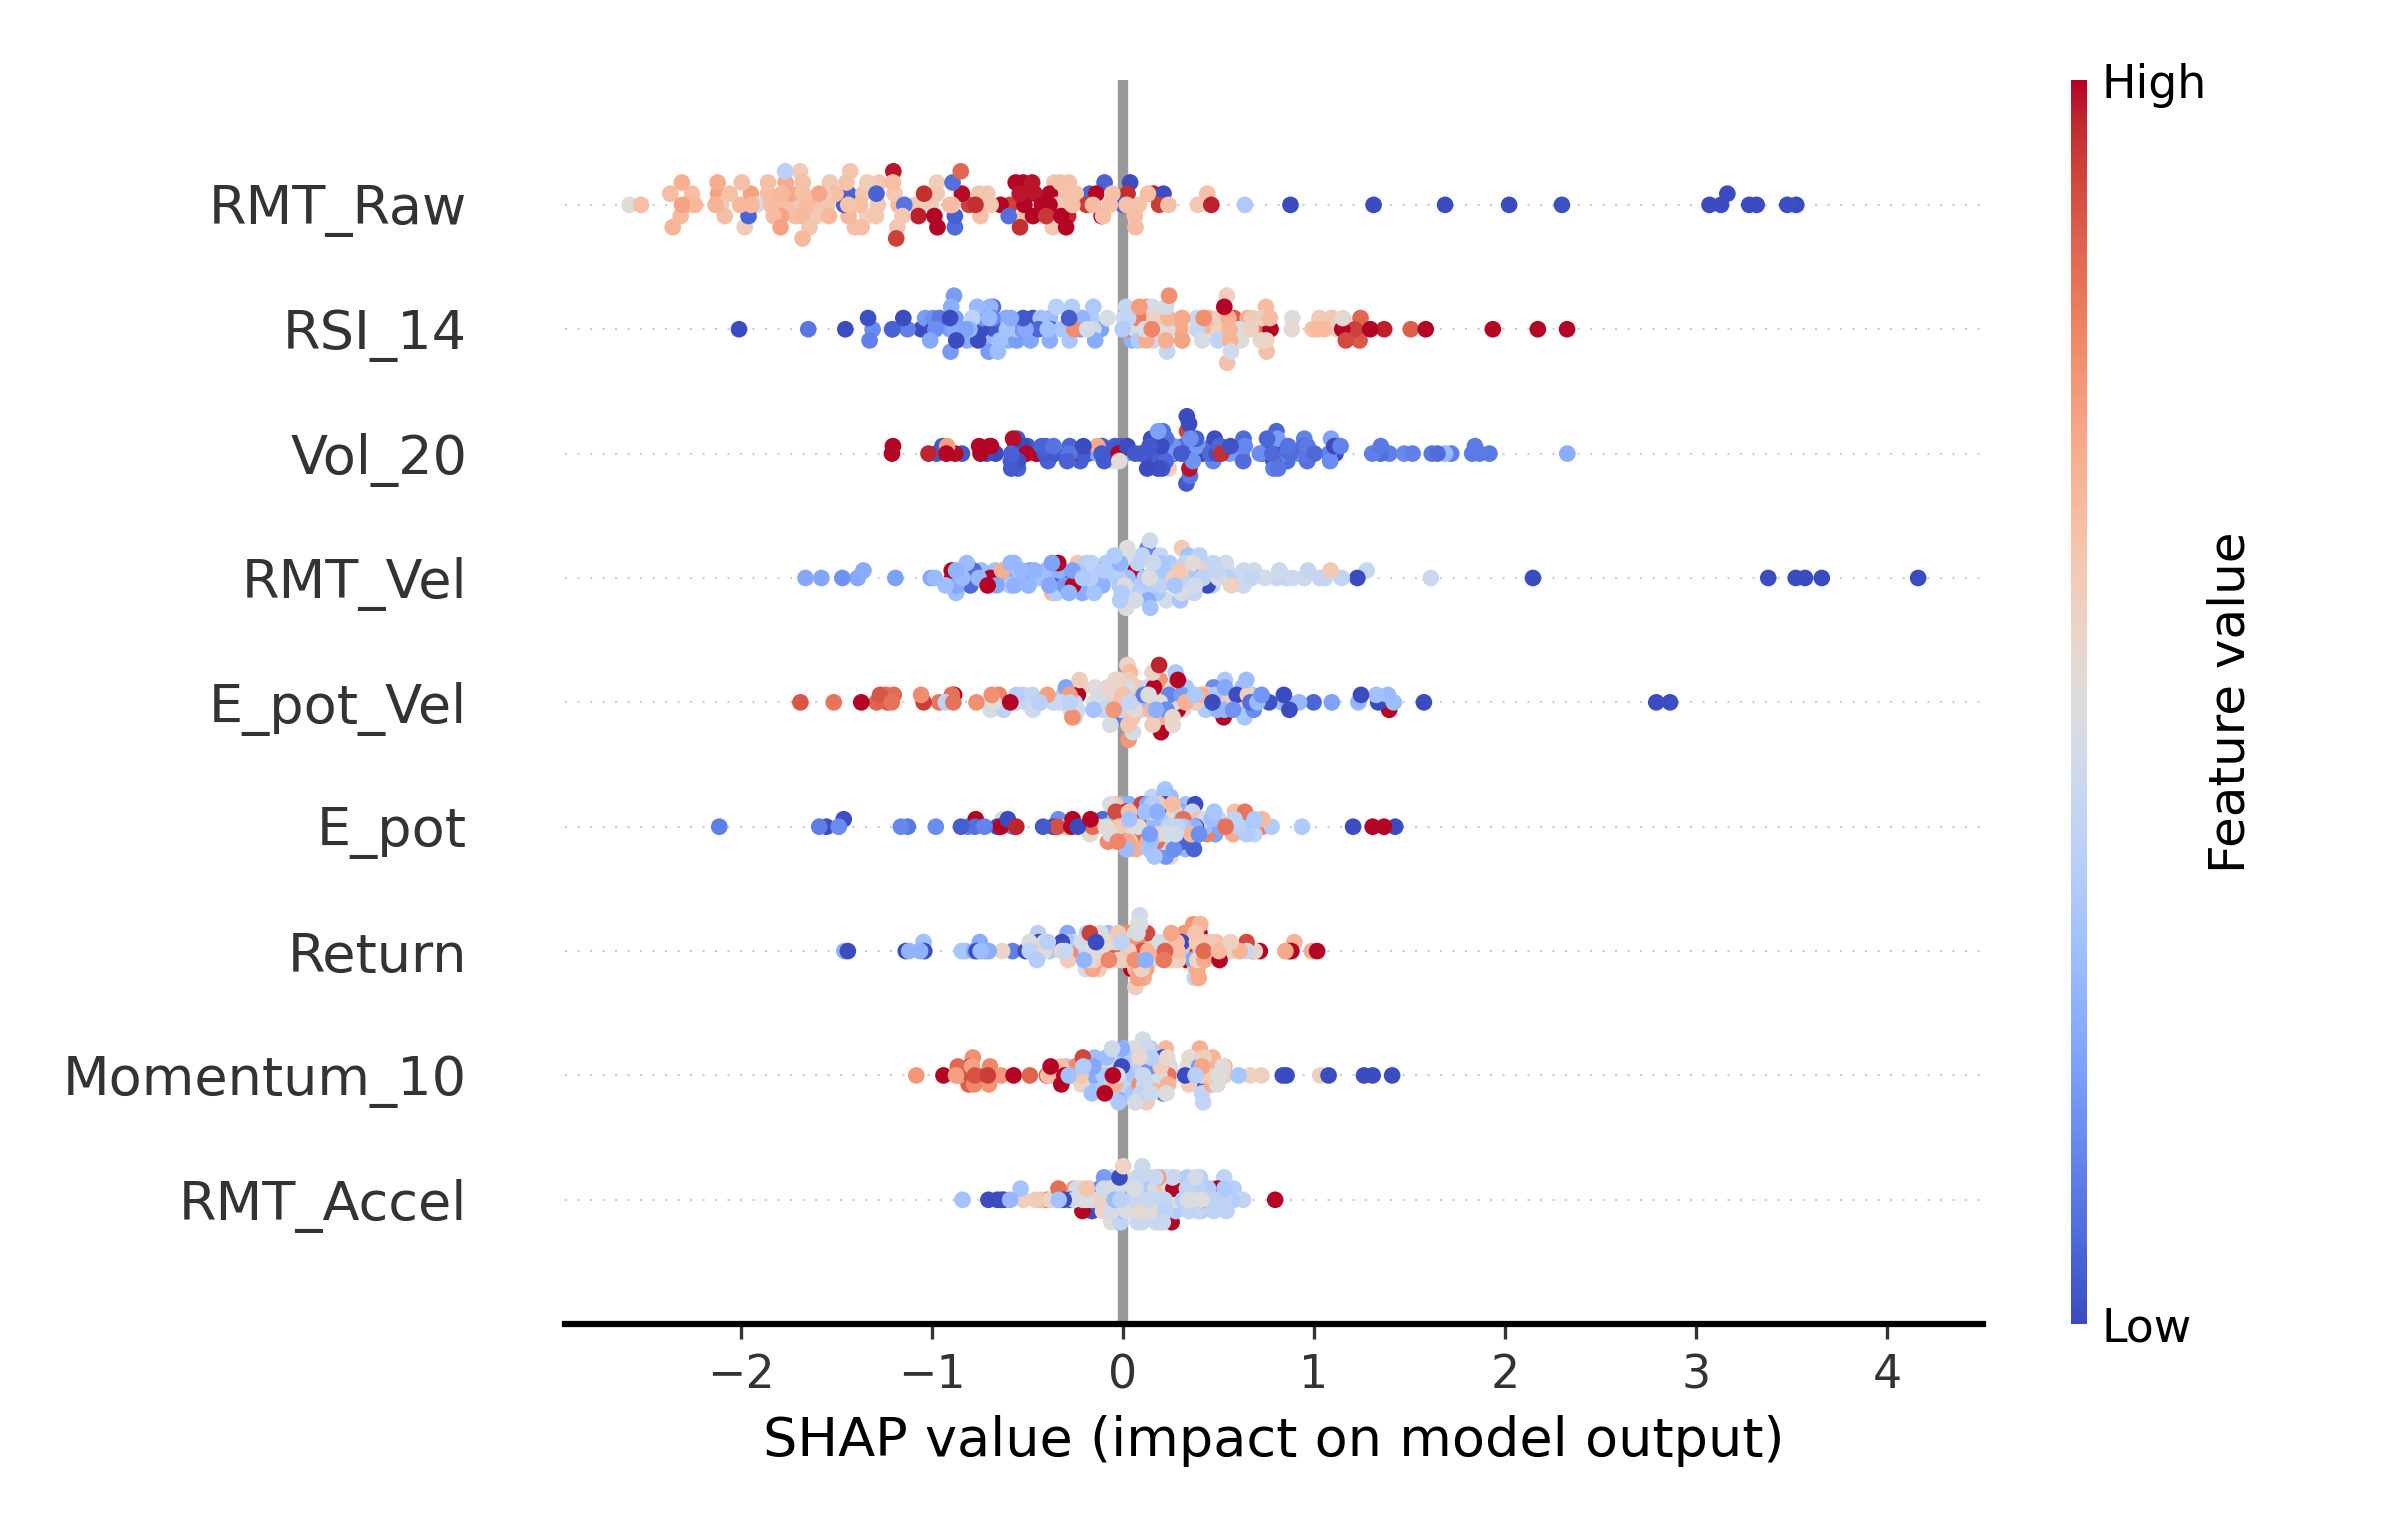
\includegraphics[width=\linewidth]{figures/fig_5_9b_shap_modelC_index2_scenario1.png}
    \caption*{(d) Index 2 / Model C}
  \end{minipage}
  \caption{シナリオ1のSHAP分析。(c)において、RMT特徴量の低い値（青色）が予測値を正に押し上げている点に注目。}
  \label{fig:shap_scenario1}
\end{figure}

ModelB(c)の結果に注目すると、RMT\_Raw（最大固有値 $\lambda_{max}$）のSHAP値は、特徴量の値が低い（青色）ときにプラス（危険）に作用し、高い（赤色）ときにマイナス（安全）に作用していることがわかる。
これは、「市場の同期が強まれば暴落する（$\lambda_{max}$ 増大＝危険）」という従来の単純な直感とは逆の結果である。このメカニズムを解明するため、次項で暴落前後の時系列推移を詳細に分析する。

\subsubsection{RMTのミクロダイナミクス：「嵐の前の静けさ」の検知}
前項のSHAP分析で示された「RMTの値が低いほど危険」という逆説的な結果を検証するため、2025年3月の暴落局面における時系列詳細解析を行った。図\ref{fig:micro_dynamics}に、(a)市場価格の推移と、(b)RMT最大固有値 $\lambda_{max}$ および提案モデルの予測確率の推移を示す。

\begin{figure}[H]
  \centering
  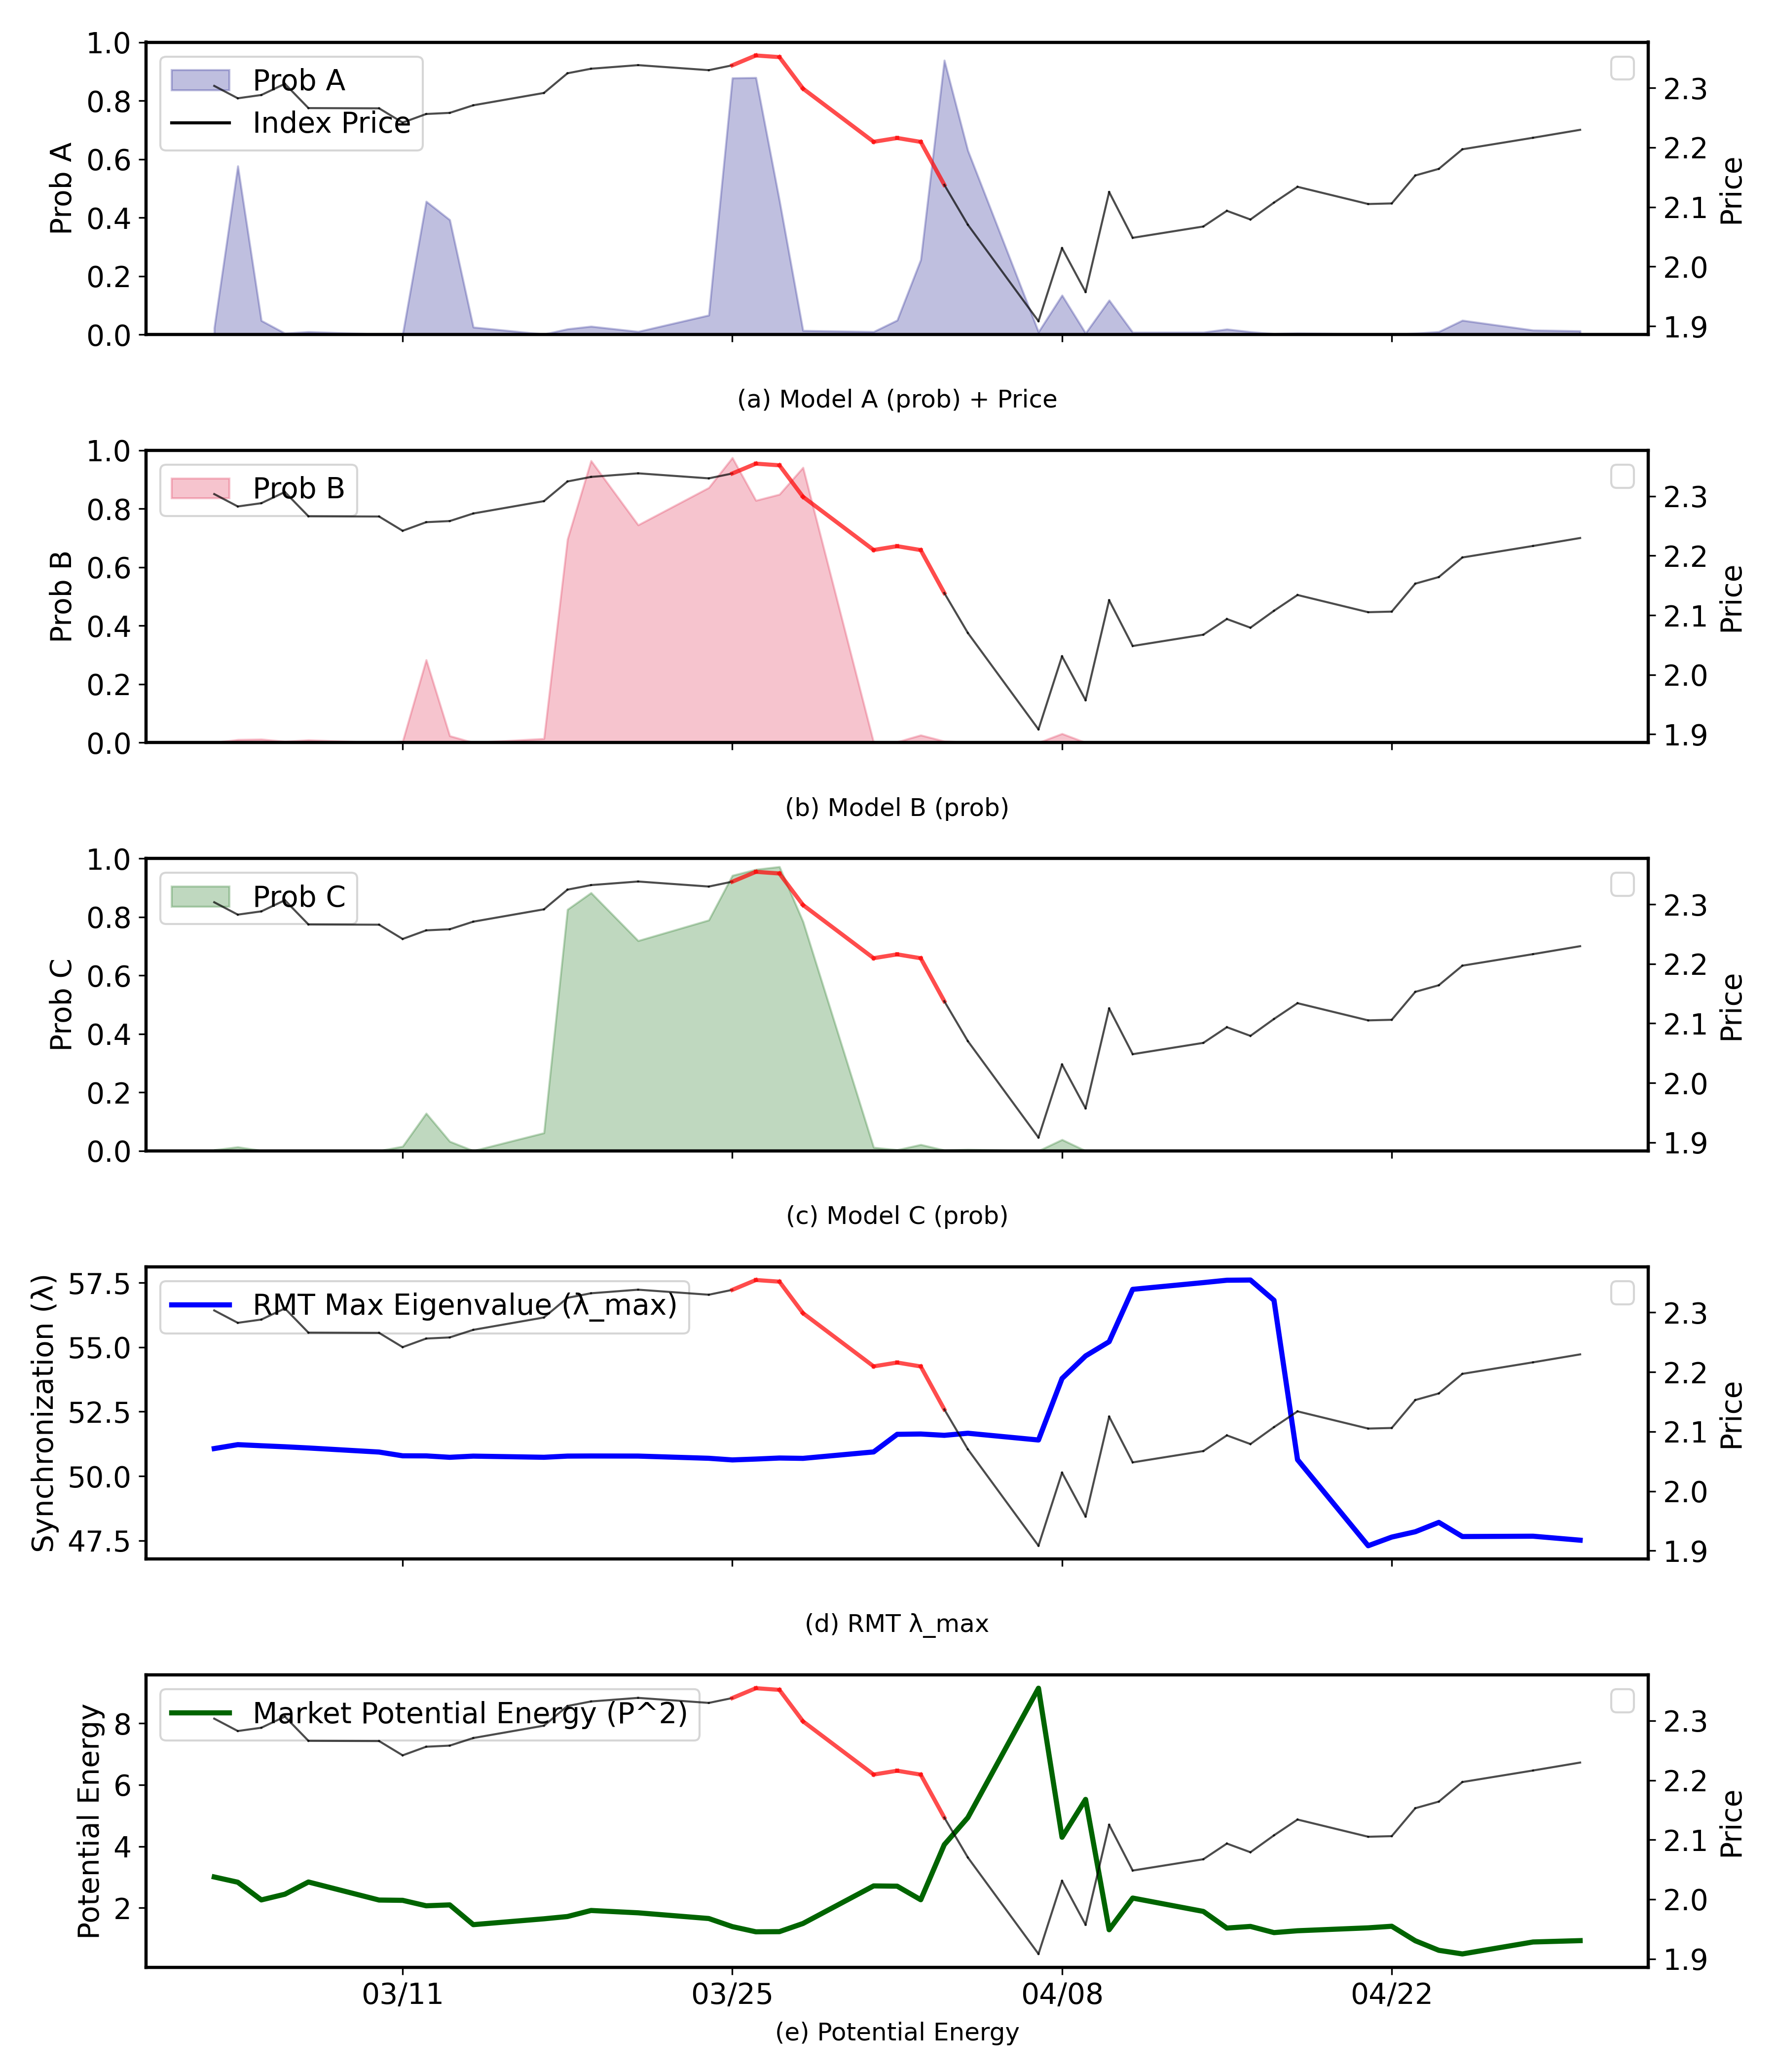
\includegraphics[width=0.95\linewidth]{figures/fig5_12a_micro_data_index1_scenario1.png}
  \caption{暴落前後（2025/3/15 -- 4/10）における詳細解析。(a)市場価格は3/25から暴落を開始。(b)RMT固有値（青実線）は暴落直前の予兆フェーズにおいて低位安定しており、これに逆相関するように予測確率（赤破線）が急上昇していることが確認できる。}
  \label{fig:micro_dynamics}
\end{figure}

図\ref{fig:micro_dynamics}(b)より、暴落プロセスは明確に以下の3フェーズに分類できる。

\begin{enumerate}
    \item \textbf{予兆フェーズ（Nucleation Phase, 3/18 -- 3/24）:}
    市場価格は高値圏にあるが、$\lambda_{max}$ は $50.6 \sim 50.8$ という局所的な最小値付近で推移している。この「不気味な静けさ（同期の低下）」をモデルは敏感に察知し、予測確率を $0.90$ 以上へと引き上げている。
    
    \item \textbf{崩壊フェーズ（Crash Phase, 3/25 -- 4/2）:}
    実際の暴落が開始。
    
    \item \textbf{緩和フェーズ（Relaxation Phase, 4/3以降）:}
    パニック売りが一巡し、$\lambda_{max}$ が $51.5$ 以上へと急上昇（再同期）すると、モデルは「リスクのピークは過ぎた」と判断し、予測確率を沈静化させている。
\end{enumerate}

さらに、この期間におけるRMT固有値と予測確率の相関を図\ref{fig:rmt_corr}に示す。

\begin{figure}[H]
  \centering
  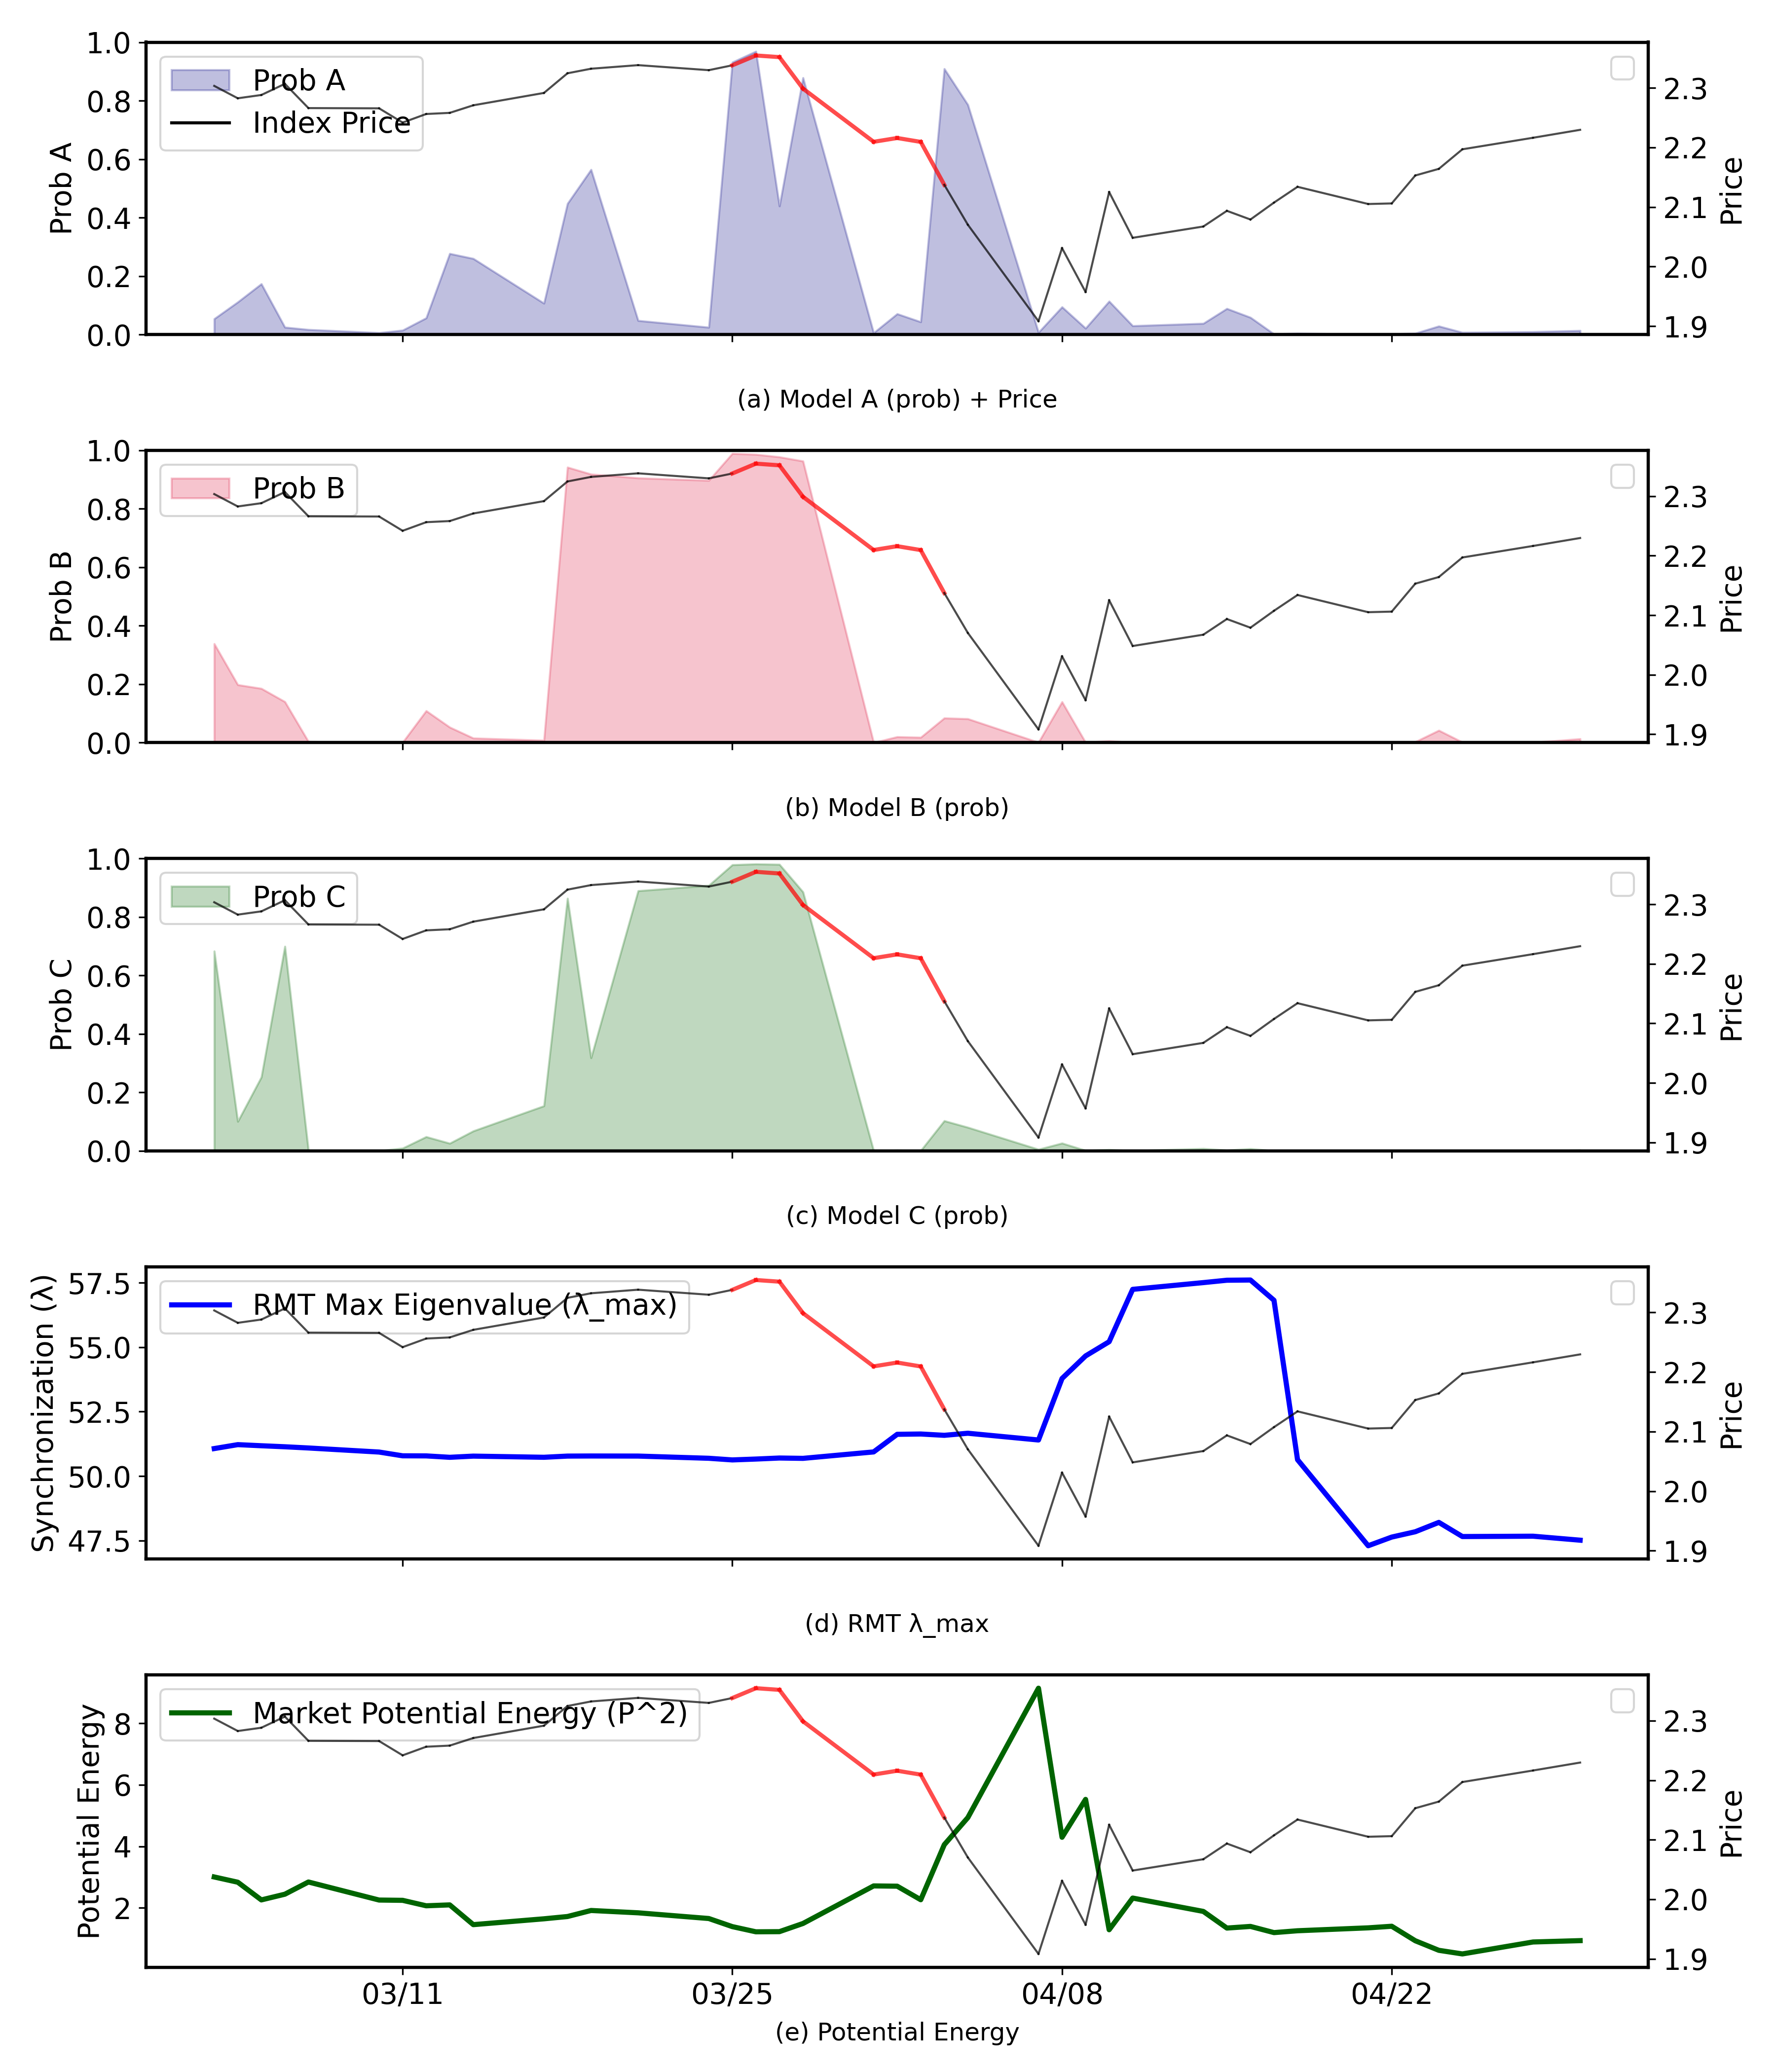
\includegraphics[width=0.7\linewidth]{figures/fig5_12b_micro_data_index2_scenario1.png}
  \caption{RMT固有値と予測確率の散布図（対象期間：2025/3/15 -- 4/10）。明確な負の相関が見られ、モデルが「低固有値状態」を「高リスク（赤色プロット）」として分離していることがわかる。}
  \label{fig:rmt_corr}
\end{figure}

これらの結果は、本モデルが単なる価格追従型のアルゴリズムではなく、統計力学的な\textbf{「相転移の前兆としての揺らぎの縮小（Critical Slowing Downの前段階としての静寂）」}を捉えていることを強く示唆するものである。
\clearpage
\bibliographystyle{unsrt}
\bibliography{references}

\end{document}